%=================================================================================
\chapter*{Note}
%=================================================================================

Le matériel présenté dans ce document consiste en une reprise, avec beaucoup d'apports personnels et de modifications, des cours présentés par les Profs. Lorenzo Zago et Jacques Unger de la HEIG-VD. Nous tenons à les remercier de nous avoir transmis l'intégralité de leurs documents de cours et laboratoire.

Ces documents ont été eux-mêmes basés sur une compilation de plusieurs sources - polycopiés pré-existants à la HEIG-VD, \texttt{Wikipédia}, et contributions d'auteurs librement disponibles sur internet.

%=================================================================================
\chapter{Introduction}
%=================================================================================

%------------------------------------------
\section{Techniques de mesure, métrologie, analyse des données}
%------------------------------------------

En ingénierie, et dans toutes les branches scientifiques, les informations sur les systèmes physiques, construits par l'humain, ou naturels, sont obtenues par des \textbf{mesures}. deux questions essentielles se posent alors à l'expérimentateur~:
\begin{enumerate}
\item comment mesurer de la manière la plus juste possible,
\item et comment déduire, des mesures brutes, l'information recherchée ?
\end{enumerate}
La première partie est du domaine de ce que nous pouvons nommer les \textbf{techniques de mesures}, accompagnée des règles de la \textbf{métrologie}. La seconde partie constitue le vaste domaine de \textbf{l'analyse des données}. Dans ce cours, nous traiterons tout d'abord des techniques des mesures, logiquement suivies de la présentation des techniques d'analyse de données.

%------------------------------------------
\section{Utilité de la métrologie}
%------------------------------------------

Les techniques de mesure ont recours à la métrologie, terme qui se traduit, au sens étymologique, par \textless\textless\ science de la mesure\ \textgreater\textgreater. Avant d'entrer dans le vif du sujet, à savoir les techniques de mesure, il est donc nécessaire de bien comprendre quels sont les défis résolus par la métrologie.

La métrologie s'intéresse traditionnellement à la détermination de caractéristiques (appelées grandeurs) qui peuvent être fondamentales comme par exemple une longueur, une masse, un temps, ou dérivées de grandeurs fondamentales comme par exemple une surface, une vitesse (notons que dans beaucoup de domaines, comme celui des essais des matériaux, la médecine ... il existe des unités spécialisées qui n'ont pas de lien forcément direct avec les unités fondamentales ci-dessus, mais qui sont néanmoins parfaitement définies).

Quoi qu'il en soit, mesurer une grandeur physique consiste à lui attribuer une valeur quantitative en prenant pour référence une grandeur de même nature appelée unité. Dans le langage courant des métrologues, on entend souvent dire \textless\textless\ mesurer c'est comparer\ \textgreater\textgreater.

\begin{figure}[ht]
   \centering
   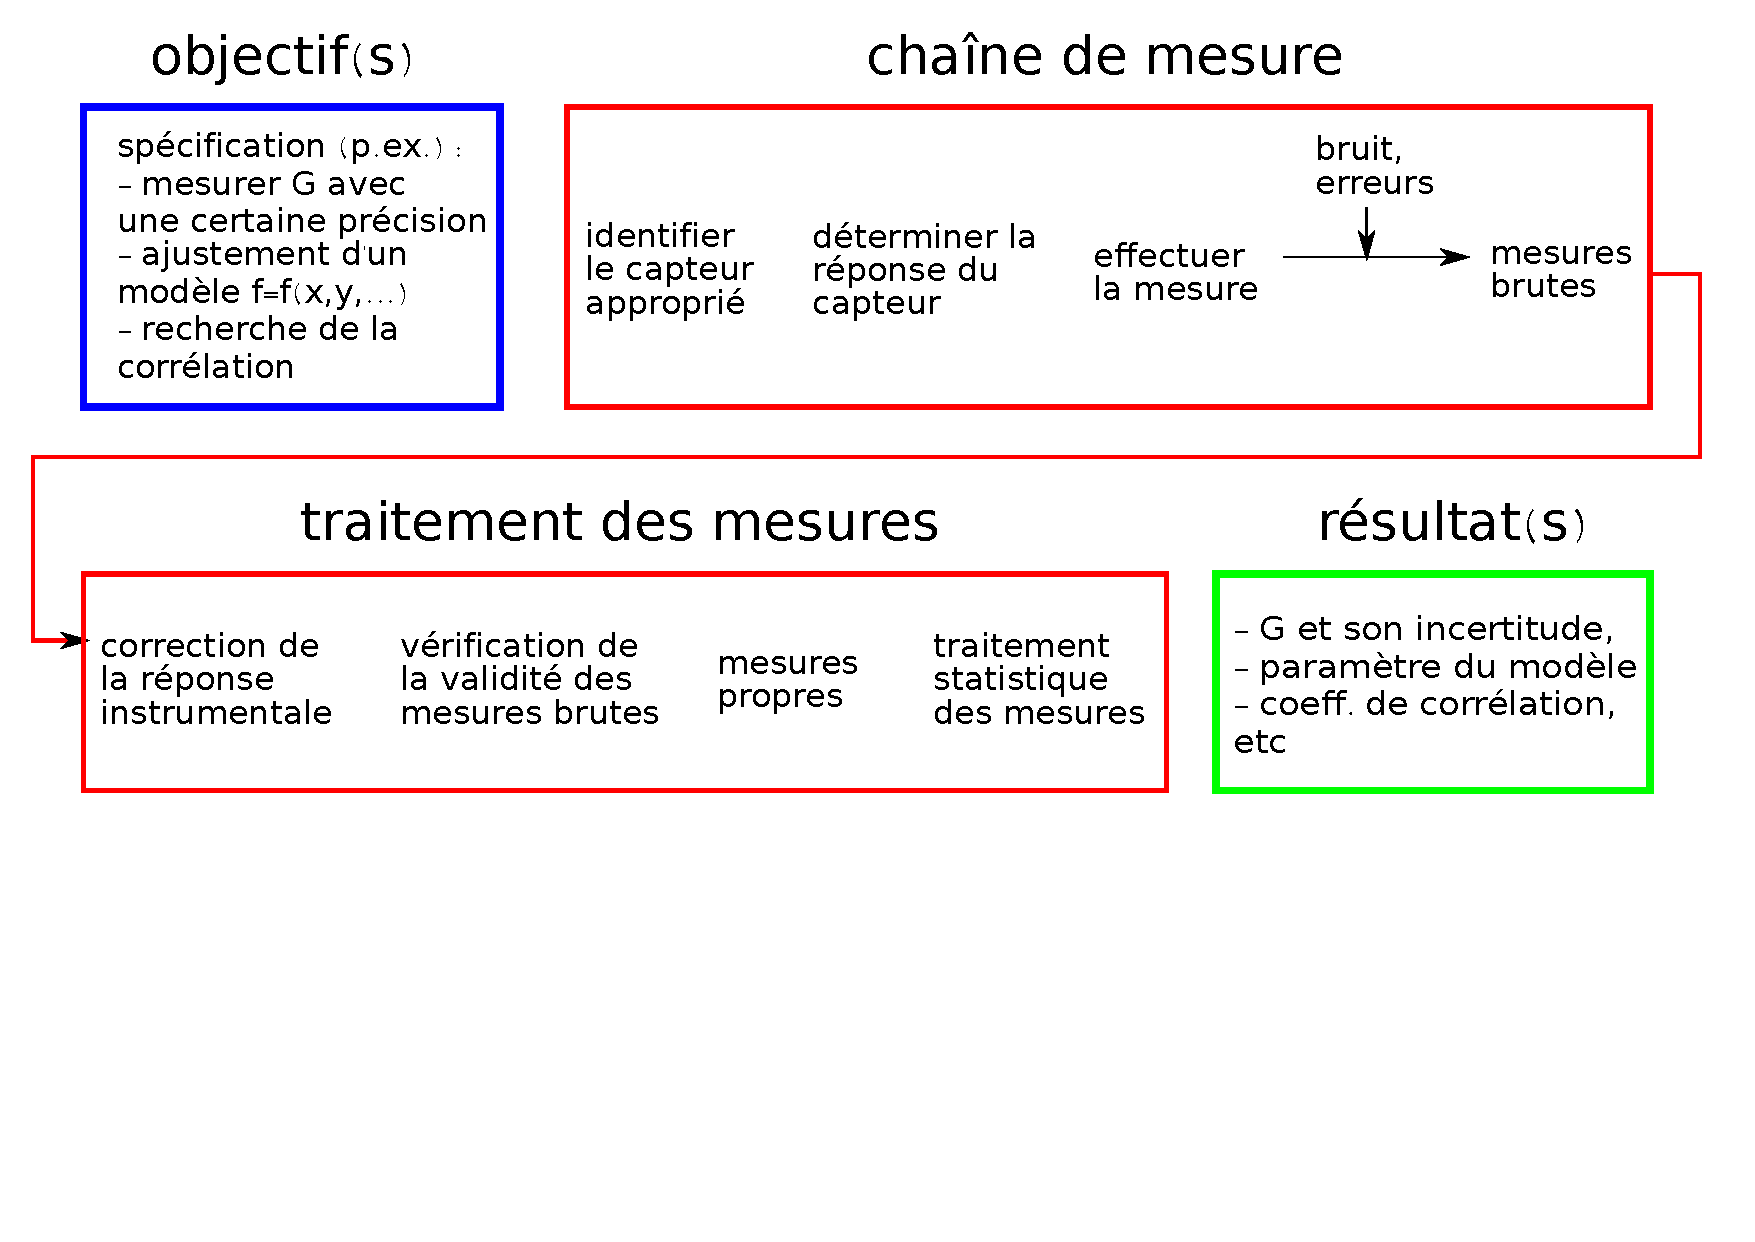
\includegraphics[width=0.9\textwidth]{assets/figures/flowChartTechMes.pdf}
   \caption{Techniques de mesure et traitement des données~: les étapes clés.}
   \label{fig:flowchartTechMes}
\end{figure}
Les résultats des mesures servent à prendre des décisions dans de nombreux domaines, tels que:
\begin{itemize}\itemsep1pt
\renewcommand{\labelitemi}{$\bullet$}
\item validation d'une hypothèse scientifique,
\item acceptation d'un produit (conformité à une exigence),
\item réglage d'un paramètre dans le cadre du contrôle d'un procédé de fabrication,
\item protection de l'environnement,
\item définition des conditions de sécurité d'un produit ou d'un système.
\end{itemize}
L'ensemble de ces décisions concourt à la qualité des produits ou des services: on peut quantifier (ou caractériser) la qualité d'un résultat de mesure grâce à son incertitude.
En effet sans incertitude les résultats de mesure ne peuvent plus être comparés:
\begin{itemize}\itemsep1pt
\renewcommand{\labelitemi}{$\bullet$}
\item soit entre eux (essais croisés),
\item soit par rapport à des valeurs de référence spécifiés dans une norme ou une spécification (conformité d'un produit).
\end{itemize}

Le diagramme de la figure  ~\ref{fig:flowchartTechMes} représente les différentes étapes nécessaires à la réalisation d'un système de mesure, depuis l'acquisition au traitement des mesures. C'est sur cette base que les chapitres ont été définis:
\begin{description}
\item[Chapitre 1] Introduction
\item[Chapitre 2] Le système international d'unités
\item[Chapitre 3] La chaîne de mesure
\item[Chapitre 4] Modélisation de la chaîne de mesure
\item[Chapitre 5] Capteurs
\end{description}

La 2e partie traitera de l'analyse des données:
\begin{description}
\item[Chapitre 6] La mesure et sa représentation
\item[Chapitre 7] La mesure vue comme une variable aléatoire. Distributions usuelles des
variables aléatoires.
\item[Chapitre 8] Mesures multidimensionnelles, corrélations, budget d'erreur
\item[Chapitre 9] Ajustement d'un modèle sur une série de mesures
\end{description}

\textbf{A la fin de ce cours, vous devriez être capable de concevoir un système de mesure d'une grandeur physique donnée, et de traiter les données enregistrées pour en tirer les informations désirées.}

%=================================================================================
\chapter{Le système international d'unité (SI)}
%=================================================================================

Le \textbf{Système International d'unités (abrégé SI)}, basé sur le \textbf{système métrique}, est le système d'unités le plus largement employé du monde. Il s'agit d'un système d'unités décimal (on passe d'une unité à ses multiples ou sous-multiples à l'aide de puissances de 10). C'est la Conférence Générale des Poids et Mesures (CGPM), rassemblant des délégués des états membres de la Convention du Mètre, qui décide de son évolution, tous les quatre ans, à Paris.

L'abréviation de \textless\textless\ Système International\ \textgreater\textgreater est SI, \textbf{quelle que soit la langue utilisée}\footnote{oui, \textit{même} en anglais}. La norme internationale ISO 1000 (ICS 01 060) décrit les unités SI et les recommandations pour l'emploi de leurs multiples et de certaines autres unités.

%------------------------------------------
\section{Les sept unités de base SI}
%------------------------------------------

%..........................................
\subsection{Origine}
%..........................................

Le nombre minimal d'unités possibles est basé sur le nombre minimal de grandeurs indépendantes et fondamentales permettant de décrire les lois de l'Univers. On comprendra aisément que l'\textbf{espace}, le \textbf{temps} et la \textbf{masse} sont des grandeurs ne pouvant pas s'exprimer les unes en fonction des autres, et que ces trois grandeurs définissent forcément \textbf{les trois premières unités fondamentales} de tout système métrologique, qui sont respectivement, en unités SI, le mètre, la seconde, le kilogramme.

Il existe une quatrième grandeur fondamentale, la \textbf{charge électrique}, irréductible aux  précédentes~: on ne peut pas traduire la charge de l'électron ou du proton en une combinaison de masse, distance, et/ou temps~! A noter que c'est l'unité du courant électrique, soit la quantité de charge électrique qui passe dans un conducteur par unité de temps, qui constitue la quatrième unité fondamentale - l'ampère (A) - et non l'unité de la charge, le coulomb (C).

Pour continuer, il existe encore d'autres grandeurs fondamentales dont on ne parle presque jamais en dehors du monde de la physique subatomique~: les charges liées aux interactions entre les particules fondamentales constitutives des protons et neutrons (les quarks), ainsi qu'entre les électrons et leur différentes versions (positron, muon etc.) Ces deux interactions se nomment l'interaction forte (pour les quarks) et faible (pour les électrons), mais ont une portée se limitant essentiellement aux dimensions du noyau de l'atome, et leurs effets ne se font ressentir que lors des expériences de physique des particules.

De la même manière que la charge électrique est le véhicule de la force électro-magnétique, il existe des charges véhiculant les interactions forte et faible (nous ne les décrirons pas ici). Or, ces charges ne sont pas exprimables en terme des 4 unités fondamentales précédentes, elles constituent par conséquent de nouvelles grandeurs indépendantes, pour lesquelles des unités sont définies. Ceci dit, étant donné que ces charges n'ont d'importance que dans le domaine spécialisé de la physique des particules, et qu'elles sont loin d'avoir des applications courantes dans le monde actuel (hormis dans le domaine de l'imagerie médicale nucléaire), ces unités ne sont pas (encore) incluses comme unités fondamentales SI.

Aux quatre unités fondamentales ci-dessus, le système SI ajoute trois autres unités, le \textbf{kelvin} pour la température, la \textbf{candela} pour les mesures photométriques (quantité de lumière) et la \textbf{mole}, pour la quantité de matière.

Formellement, le kelvin et la candela ne sont pas des unités fondamentales~: la température est en fait une mesure de l'énergie d'agitation thermique (oscillation, vitesse) des particules constituantes d'un corps à une température donnée; un flux de lumière n'est rien d'autre qu'un flux de photons véhiculant une certaine énergie. Or, l'énergie est exprimable en terme de distance, de masse et de temps.

La mole est en revanche une unité assez particulière, puisqu'elle ne correspond à aucune grandeur fondamentale des lois de la physique, au contraire des unités ci-dessus. Elle trouve son origine en chimie, où l'on a trouvé bien plus pratique, pour désigner un nombre d'atomes ou de molécules au sein d'une solution, de les regrouper par rapport à un nombre de base, très grand, le nombre d'Avogadro, égal à $6.022141293\times 10^{23}$, typique du nombre d'atomes/molécules que l'on trouve dans les préparations de chimie\footnote{on consultera avec intérêt la page Wikipédia dédiée à ce sujet}. Il est en effet par exemple plus simple d'indiquer qu'il y a 3.5 moles d'une certaine molécule dans une solution donnée que de dire qu'il y en a $21.08\times 10^{23}$.

%..........................................
\subsection{Définitions}
%..........................................

Considérons l'unité de distance fondamentale, le mètre. Afin que cette référence soit disponible partout dans le monde, nous pourrions par exemple reproduire le mètre étalon conservé au \textbf{Bureau International des Poids et Mesures (BIPM)} à Sèvres, France. Cette procédure présente cependant deux inconvénients majeurs : (1) tout procédé de reproduction ne saurait être exempt d'erreurs, (2) il faut avoir accès au mètre-étalon.

Pour pallier à ces inconvénients, il a été décidé de définir le mètre non plus par rapport à un étalon physique, un objet bien réel, mais d'utiliser une propriété fondamentale de la matière, indépendante du temps et de l'espace, c'est-à-dire disponible partout et tout le temps, et parfaitement invariable, ou constante. On a donc choisi de définir le mètre comme la distance parcourue par la lumière, dans le vide, durant $1/299'792'458$ secondes exactement. Tout laboratoire bien équipé pourra reproduire cette expérience, et donc définir avec toute la précision requise une distance, entre deux plans de référence bien accessibles, égale au mètre ou à un de ses multiples ou sous-multiples.

L'exemple du mètre décrit le principe que l'on applique aujourd'hui à la définition des unités fondamentales SI. Seul le kilogramme est encore défini par rapport à un objet matériel concret – une masse composée d'un alliage de platine et d'iridium conservé au BIPM - susceptible de s'altérer. Des recherches ont d'ailleurs actuellement lieu pour remplacer cette définition par une autre, utilisant cette fois un phénomène physique, inaltérable par nature.

\newpage

\begin{center}
\begin{tabular}[t]{>{\pbs\raggedright}p{2.5cm}
                   >{\pbs\centering}p{2.2cm}
                   >{\pbs\centering}p{2.3cm}
                   >{\pbs\raggedright}p{7cm}}
\hline\hline
\textbf{Grandeur} & \textbf{Nom} & \textbf{Symbole SI} & \textbf{Définition, remarques}\\
\hline
longueur & mètre & m &
Le mètre est la longueur du trajet parcouru dans le vide par la lumière pendant 1/299'792'458 seconde. Historiquement, la première définition officielle du mètre (1791) était basée sur la circonférence de la terre, et valait 1/40'000'000 du périmètre de notre planète.
\\ \hline
masse & kilogramme & kg &
Le kilogramme est la masse d'un cylindre composé d'un alliage de platine (90 \%) et d'iridium (10\%), conservé au Bureau International des Poids et Mesures. Historiquement, la définition du kilogramme était la masse d'un décimètre cube d'eau.
\\ \hline
temps & seconde & s &
La seconde est la durée de temps associée à 9'192'631'770 oscillations de l'onde électro-magnétique (photons) émise lors de la transition des électrons entre les deux sous-niveaux d'énergie de l'état d'énergie fondamental de l'atome de césium 133 ($^{133}$Cs) à la température de 0 kelvin. La seconde était à l'origine basée sur la durée (instable) du jour terrestre, d'une durée de 86'400 secondes.
\\ \hline
\end{tabular}
\end{center}
\begin{center}
\begin{tabular}[t]{>{\pbs\raggedright}p{2.5cm}
                    >{\pbs\centering}p{2.2cm}
                    >{\pbs\centering}p{2.3cm}
                    >{\pbs\raggedright}p{7cm}}
\hline
courant électrique & ampère & A &
L'ampère est l'intensité d'un courant constant qui, maintenu dans deux conducteurs parallèles, rectilignes, de longueur infinie, de section circulaire négligeable et placés à une distance de un mètre l'un de l'autre dans le vide produirait entre ces conducteurs une force égale à $2\times10^{-7}$ newton par mètre de longueur.
\\ \hline
température & kelvin & K	&
Le kelvin, unité de température thermodynamique, est la fraction 1/273.16 de la température thermodynamique du point triple de l'eau. Le point triple de l'eau est, dans le diagramme pression-température, un point où l'eau peut exister dans les trois états, soit solide, liquide et gazeux. La température associée à cet état est de 273.16 K. A noter que l'on écrit K et non $^{\circ}$K.
\\ \hline
quantité de matière & mole & mol	&
La mole est la quantité de matière d'un système contenant autant d'entités élémentaires qu'il y a d'atomes dans 0.012 kg de carbone 12 ($^{12}$C). Ce nombre d'entités élémentaires est appelé nombre d'Avogadro, et vaut $\mathcal{N}_{A}=6.02214129(27)\times10^{23}\,\text{mol}^{-1}$. Lorsque l'on emploie la mole, les entités élémentaires doivent être spécifiées et peuvent être des atomes, des molécules, des ions, des électrons, d'autres particules ou des groupements spécifiés de telles particules.
\\ \hline
\end{tabular}
\end{center}
\begin{center}
\begin{tabular}[t]{>{\pbs\raggedright}p{2.5cm}
                    >{\pbs\centering}p{2.2cm}
                    >{\pbs\centering}p{2.3cm}
                    >{\pbs\raggedright}p{7cm}}
\hline
intensité lumineuse & candela & cd &
La candela est l'intensité lumineuse, dans une direction donnée, d'une source qui émet un rayonnement monochromatique de fréquence $540\times10^{12}$ hertz et dont l'intensité énergétique dans cette direction est de 1/683 watt par stéradian.
\\ \hline\hline
\end{tabular}
\end{center}

%------------------------------------------
\section{Unités dérivées}
%------------------------------------------

Les unités dérivées font partie du système SI et sont déduites des sept unités de base.
\begin{center}
\begin{tabular}[t]{>{\pbs\raggedright}p{28mm}
                    >{\pbs\centering}p{15mm}
                    >{\pbs\centering}p{12mm}
                    >{\pbs\centering}p{22mm}
                    >{\pbs\centering}p{22mm}
                    >{\pbs\raggedright}p{32mm}}
\hline\hline
\textbf{Grandeur} & \textbf{Nom} & \textbf{Sym. SI} & \textbf{lien avec autres unités} & \textbf{lien avec unités de base} & \textbf{Relation physique}\\
\hline
Fréquence & hertz & Hz & --- & 1/s & Fréquence = 1/période \\ \hline
Force & newton & N & --- & kg m/s$^2$ & Force = masse $\times$ accélération \\ \hline
Contrainte, pression & pascal & Pa	& N/m$^2$ & kg/m/s$^2$ & Pression = force / surface \\ \hline
Energie, travail, quantité de chaleur & joule & J & N m & kg m$^2$/s$^2$	& Travail = force$\times$distance;
énergie cinétique = masse$\times$vitesse$^2$/2 \\ \hline
Puissance, flux énergétique et flux thermique & watt & W & J/s & kg m$^2$/s$^3$ & Puissance = travail / temps \\ \hline
Charge électrique, quantité d'électricité & coulomb & C & --- & A s & Charge = courant$\times$temps \\ \hline
\end{tabular}
\end{center}

\begin{center}
\begin{tabular}[t]{>{\pbs\raggedright}p{28mm}
                    >{\pbs\centering}p{17mm}
                    >{\pbs\centering}p{11mm}
                    >{\pbs\centering}p{22mm}
                    >{\pbs\centering}p{22mm}
                    >{\pbs\raggedright}p{32mm}}
\hline
Force électromotrice, différence de potentiel (tension) & volt & V & J/C & kg m$^2$/s$^3$/A & Tension = travail / charge
\\ \hline
Résistance électrique & ohm & $\Omega$ & V/A & kg m$^2$/s$^3$/A$^2$ & Résistance =  tension / courant
\\ \hline
Conductance électrique & siemens & S	& A/V & s$^3$A$^2$/kg/m$^2$ & Conductance = courant / tension
\\ \hline
Capacité électrique & farad & F & C/V & s$^4$A$^2$/kg/m$^2$ & Capacité = charge / tension
\\ \hline
Induction magnétique & tesla & T	& V s/m$^2$ & kg/s$^2$/A & Induction = tension$\times$temps / surface
\\ \hline
Flux d'induction magnétique & weber & Wb	& V s & kg m$^2$/s$^2$/A & Flux d'induction = tension$\times$temps
\\ \hline
Inductance électrique & henry & H & V s/A & kg m$^2$/s$^2$/A$^2$ & Inductance = tension$\times$temps / courant
\\ \hline
Température & degré Celsius & $^{\circ}$C & --- & K & T [$^{\circ}$C]=T [K]-273.15
\\ \hline
Flux lumineux & lumen & lm & --- & cd sr & ---
\\ \hline
Eclairement lumineux & lux & lx & --- & cd sr/m$^2$ & ---
\\ \hline
Nombre de désintégrations par seconde (radioactivité) & becquerel & Bq & --- & 1/s & ---
\\ \hline
Dose de radioactivité absorbée & gray & Gy & J/kg & m$^2$/s$^2$ & ---
\\ \hline
Equivalent de dose radioactivité absorbée & sievert & Sv & J/kg & m$^2$/s$^2$ & ---
\\ \hline
Activité catalytique & katal & kat & --- & mol/s & ---
\\ \hline\hline
\end{tabular}
\end{center}

%------------------------------------------
\section{Préfixes du système SI}
%------------------------------------------

Les préfixes du système international d'unités simplifient la manipulation des mesures qui ont des rapports élevés d'unité (par exemple de 0.1 cm à 1'000 m). Ces préfixes renvoient à des multiples et des fractions de 10 ou de 1000.  Les préfixes et noms correspondants sont donnés dans le tableau ci-après. On notera que les préfixes s'écrivent avec une lettre minuscule à partir et en-dessous de l'échelle des milliers. \textbf{Il est fondamental d'observer très exactement ces conventions internationales}.

\begin{table}[htbp]
%\footnotesize
\begin{center}
\begin{tabular}{>{\pbs\raggedright}p{1cm}>{\pbs\raggedright}p{1.4cm}>{\pbs\centering}p{1.5cm}ll}
$10^n$ & Préfixe & Sym. SI & Nombre décimal & Echelle \\ \hline
$10^{24}$  & yotta &     Y & 1'000'000'000'000'000'000'000'000 & Quadrillion \\
$10^{21}$  & zetta &     Z & 1'000'000'000'000'000'000'000 & Trilliard \\
$10^{18}$  &   exa &     E & 1'000'000'000'000'000'000 & Trillion \\
$10^{15}$  &  péta &     P & 1'000'000'000'000'000 & Billiard \\
$10^{12}$  &  téra &     T & 1'000'000'000'000 & Billion \\
$10^{9}$   &  giga &     G & 1'000'000'000 & Milliard \\
$10^{6}$   &  méga &     M & 1'000'000 & Million \\
$10^{3}$   &  kilo &     k & 1'000 & Millier \\
$10^{2}$   & hecto &     h & 100 & Cent \\
$10^{1}$   &  déca &    da & 10 & Dix \\
$10^{0}$   &   --  &    -- & 1 & Unité \\
$10^{-1}$  &  déci &     d & 0.1	& Dixième \\
$10^{-2}$  & centi &     c & 0.01 & Centième \\
$10^{-3}$  & milli &     m & 0.001 & Millième \\
$10^{-6}$  & micro & $\mu$ & 0.000'001 & Millionième \\
$10^{-9}$  &  nano &     n & 0.000'000'001 & Milliardième \\
$10^{-12	}$ &  pico &     p & 0.000'000'000'001 & Billionième \\
$10^{-15	}$ & femto &     f & 0.000'000'000'000'001 & Billiardième \\
$10^{-18	}$ &  atto &     a & 0.000'000'000'000'000'001 & Trillionième \\
$10^{-21	}$ & zepto &     z & 0.000'000'000'000'000'000'001 & Trilliardième \\
$10^{-24	}$ & yocto &     y & 0.000'000'000'000'000'000'000'001 & Quadrillionième \\ \hline
\end{tabular}
\end{center}
\end{table}

\newpage

%------------------------------------------
\section{Unités angulaires}
%------------------------------------------

\begin{wrapfigure}[20]{l}[0pt]{5cm}
   \centering
   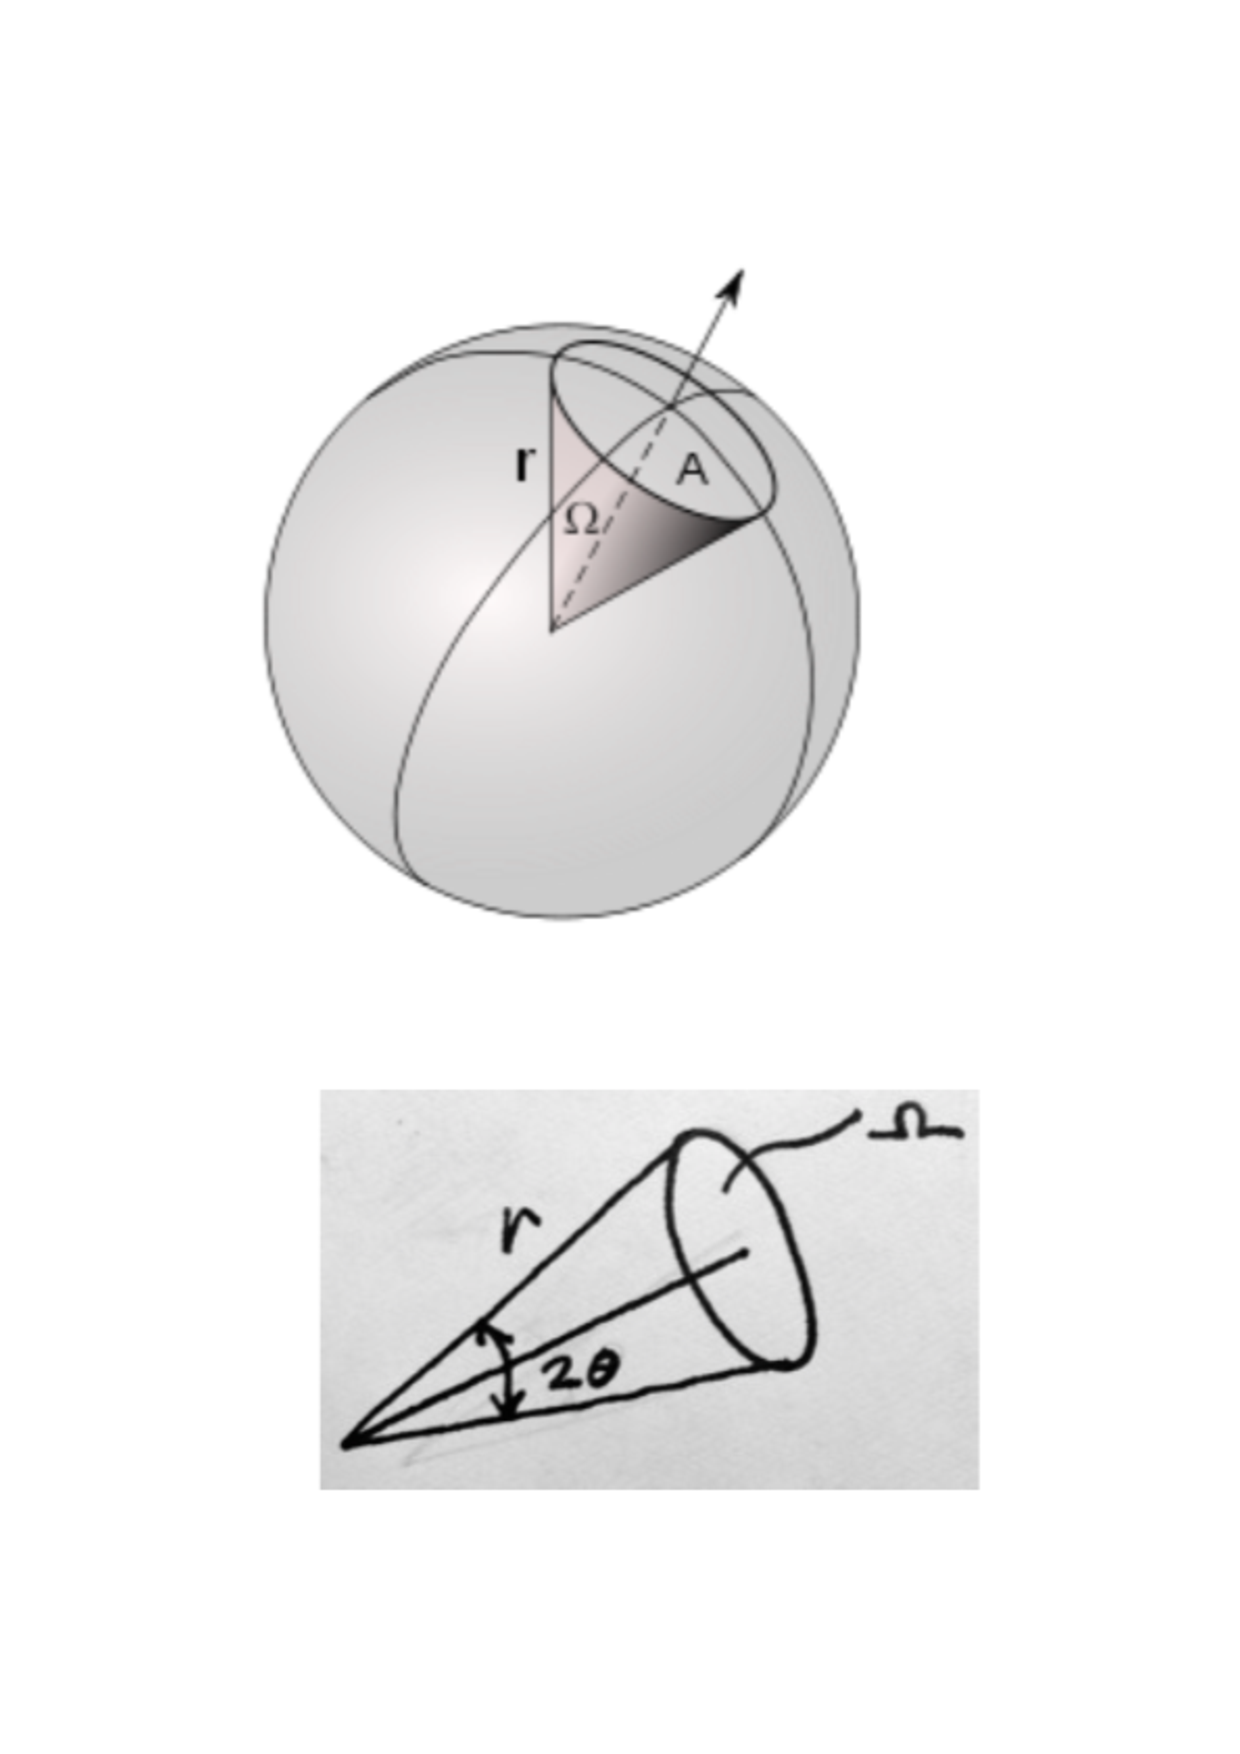
\includegraphics[width=5cm]{assets/figures/defAngleSolide.pdf}
   \caption{Définition de l'angle solide.}
   \label{fig:angles}
\end{wrapfigure}
A côté des unités de base et des unités dérivées, il existe deux unités angulaires~:

\paragraph{L'unité d'angle plan~: le radian (symbole: rad)} Soit un secteur de cercle de rayon $r$ et de longueur d'arc $l$. L'angle $\theta$ associé au secteur, en radian, est défini par le rapport
$$
\theta=\frac{l}{r}\ \ [\text{rad}]
$$
180$^\circ$ correspondant à $\pi$ rad, on a que 1 rad $\approx$ 57.3$^\circ$.

\paragraph{L'unité d'angle solide~: le stéradian (symbole: sr)} Soit un cône dont l'angle au sommet est de $2\theta$ [rad], et soit $A$ l'aire de la calotte sphérique formée par l'intersection du cône avec la surface de la sphère de rayon $r$ (figure~\ref{fig:angles}). L'angle solide $\Omega$ associé au cône est défini par le rapport
$$
\Omega=\frac{A}{r^2}\ \ [\text{sr}]
$$
L'aire d'une sphère de rayon $r$ étant donnée par $4\pi\,r^2$, on trouve que l'angle solide de la sphère est égal à $4\pi$ sr, et de la demi-sphère, $2\pi$. On peut aussi montrer que
$$
\Omega=2\pi(1-\cos\theta)
$$

Les grandeurs \textless\textless\ angle plan \ \textgreater\textgreater et \textless\textless\ angle solide \ \textgreater\textgreater sont des unités sans dimension - puisqu'il s'agit de rapport de longueurs et de surface - qui peuvent être indiquées ou non dans les expressions des unités dérivées.

%------------------------------------------
\section{Règles d'écriture des unités et symboles SI}
%------------------------------------------

\begin{itemize}\itemsep1pt
\renewcommand{\labelitemi}{$\bullet$}
\item le nom de l'unité est un nom commun même pour les unités provenant de noms propres : volt, ampère, kelvin, tesla etc;
\item les symboles SI des unités sont écrits en police droite, et en minuscules, \textbf{sauf} si le nom de l'unité est dérivée d'un nom propre~: dans ce cas la première lettre du symbole est en majuscule, par exemple N (Newton), J (Joule), V (Volta), Bq (Bequerel);
\item les symboles SI sont invariables au pluriel;
\item les symboles SI sont écrits sans point final;
\item les symboles SI doivent être placés après les valeurs numériques, en laissant un espace entre valeur et symbole, donc 30 m est juste, 30m ne l'est pas;
\item le produit de 2 unités est indiqué par un point, qui peut être omis si aucune confusion n'est possible, par exemple 1 mN est un millinewton et non un mètre-newton (c-à-d un joule), sinon nous aurions écrit m$\cdot$N !
\item le quotient est indiqué par une barre oblique, ou alors on peut utiliser les puissances négatives, comme avec m/s$^2$ ou m$\cdot$s$^{-2}$, mais pas ms$^{-2}$ car alors ms peut être interprété comme indiquant des millisecondes;
\item lorsque l'unité suit une valeur numérique, on ne met \textbf{jamais} de crochets autour de l'unité; on ne place l'unité entre crochets que dans les formules, par exemple la fameuse formule d'Einstein s'écrira
$$
E=mc^2\ \text{[J]}\ \ \ \ \text{mais par contre}\ \ \ \ E=10^6\ \text{J}
$$
\end{itemize}
Quelques exemples d'écriture  fausses et justes~:
\begin{center}
\begin{tabular}{lll}
faux & juste & interprétation\\\hline
$99Kg$& 99 kg & 99 kilogramme\\
$25 [ms]$ & 25 ms & 25 milliseconde\\
$12 \mu v$ & 12 $\mu$V & 12 microvolt\\
100 K*m & 100 K$\cdot$m & 100 kelvin$\cdot$mètre\\\hline
\end{tabular}
\end{center}

%=================================================================================
\chapter{La chaîne de mesure}
%=================================================================================

\begin{figure}[ht]
   \centering
   \vspace{-5mm}
   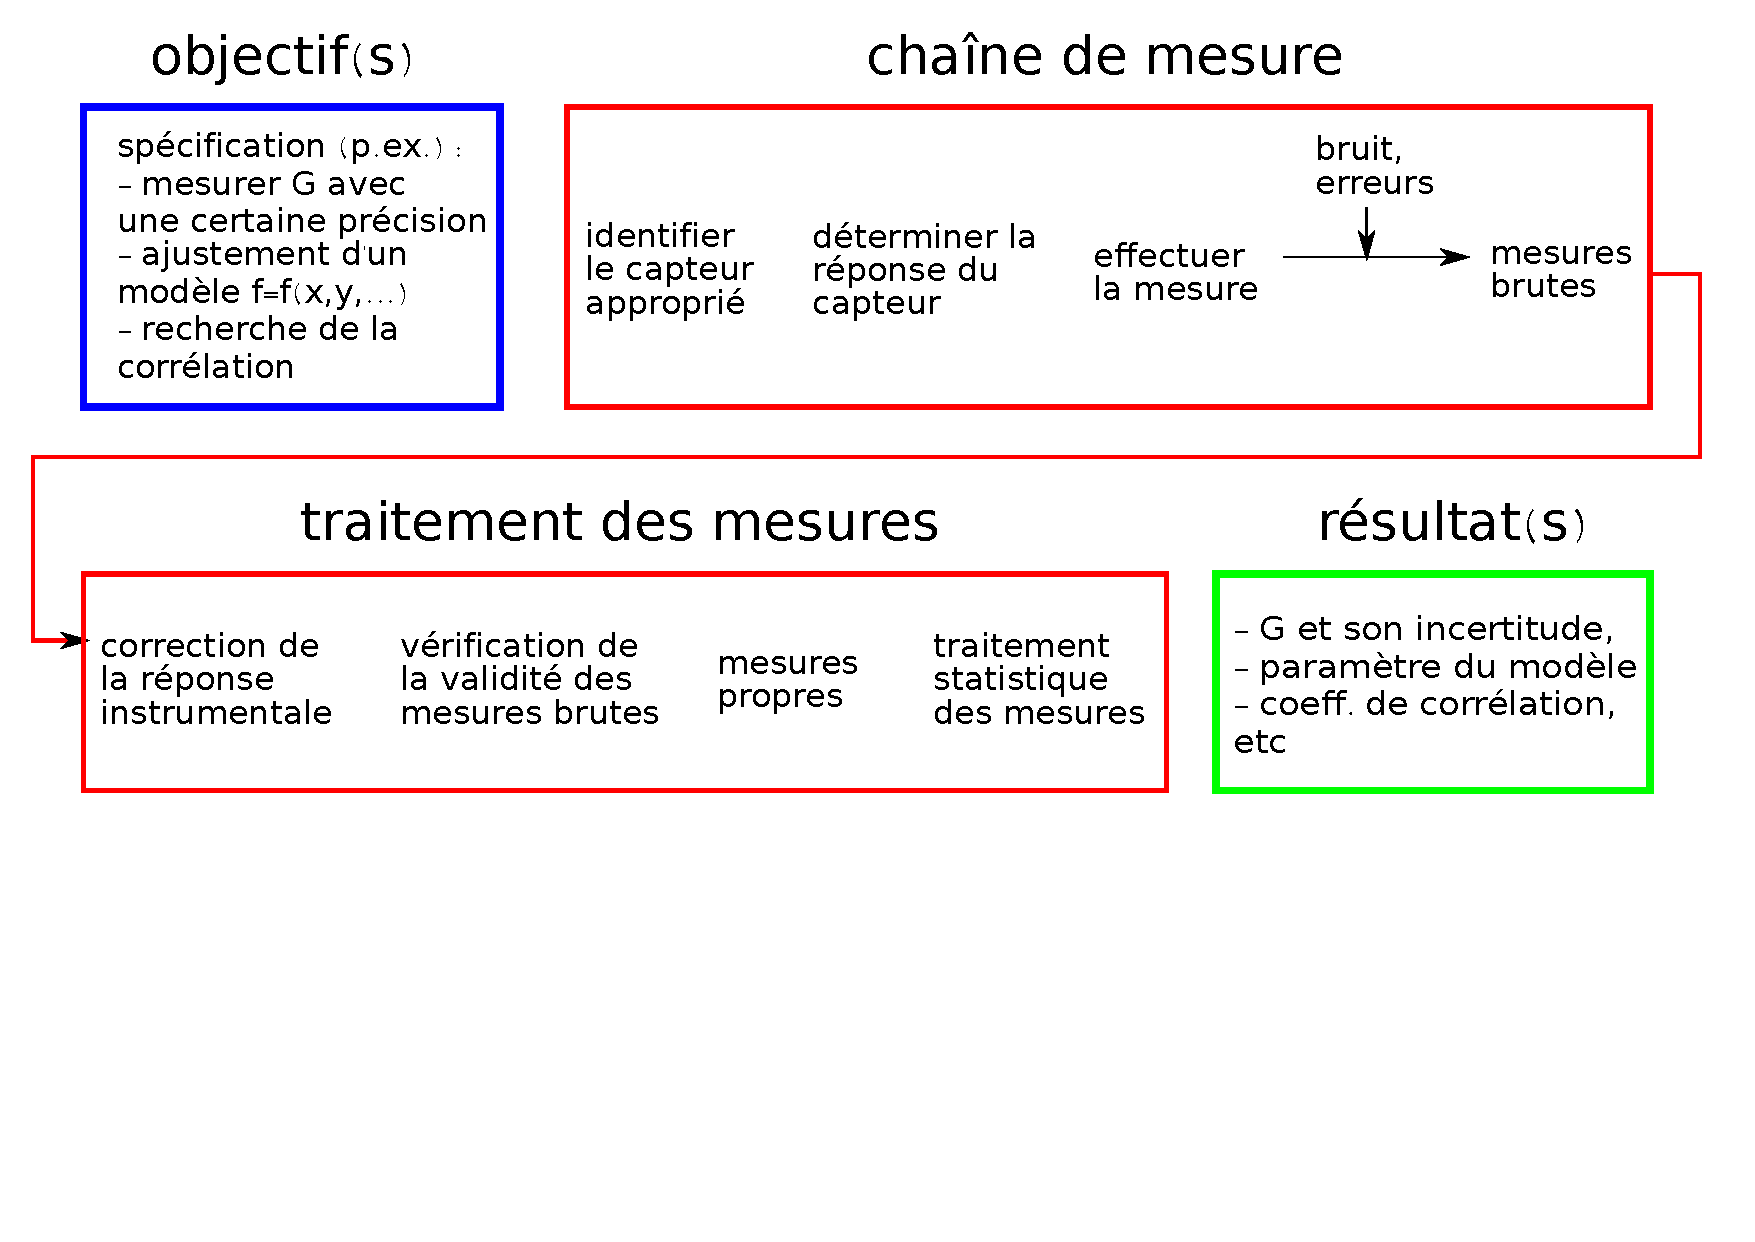
\includegraphics[width=\textwidth]{assets/figures/flowChartTechMes.pdf}
   \caption{Techniques de mesure~: les étapes clés.}
   \label{fig:flowChartTechMes_chaine_de_mesure}
\end{figure}

%------------------------------------------
\section{Introduction}
%------------------------------------------

Nous avons vu au chapitre précédent les différents moyens et définitions nécessaires pour que tous les acteurs des techniques de mesure puissent oeuvrer en se comprenant les uns les autres. Reprenant le schéma bloc de la figure \ref{fig:flowChartTechMes_chaine_de_mesure} qui présente les différentes étapes des opérations de mesure, nous nous proposons maintenant d'étudier la chaîne de mesure.

Dans l'instrumentation moderne, on constate pratiquement que chaque équipement ou appareil de mesure comprend un ou plusieurs microprocesseurs. Il convient donc, à l'intérieur du système de mesure de convertir le signal analogique représentant la grandeur que l'on veut mesurer, en une valeur numérique que l'on pourra traiter dans le processeur. Les signaux de sortie d'un capteur sont généralement petits, il est donc nécessaire de les amplifier. D'autre part le capteur doit être placé à un endroit bien précis du processus, à une distance appréciable de l'équipement de mesure (de l'ordre du mètre - p.e. oscilloscope, à plusieurs centaines de mètres - pour de grands systèmes).

Il faut donc transmettre l'information entre le capteur et le système de mesure proprement dit. L'information concernant la grandeur à mesurer va ainsi traverser une série d'éléments et d'appareils avant d'apparaître comme résultat de mesure. Cette succession d'appareils ou éléments est appelée une \textbf{chaîne de mesure}.

\begin{center}
\fbox{
\begin{minipage}{0.96\textwidth}
\textbf{\textit{Déf}. Chaîne de mesure :} succession d'appareils et d'éléments assurant la transmission et la transformation de l'information entre le capteur et le résultat de mesure.
\end{minipage}
}
\fbox{
\begin{minipage}{0.96\textwidth}
\textbf{\textit{Déf}. Mesurande  X (measurand) :} grandeur d'entrée que l'on désire mesurer
\end{minipage}
}
\end{center}

\begin{figure}[h]
   \centering
   \vspace{-5mm}
   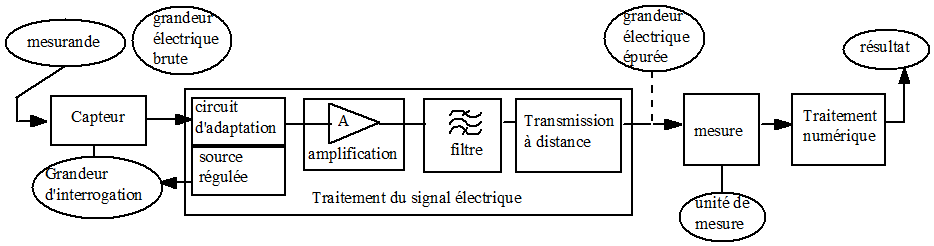
\includegraphics[width=\textwidth]{assets/figures/1_1_chaine_de_mesure.png}
   \caption{Eléments d'une chaîne de mesure. De gauche à droite~: le \textbf{capteur}, puis le bloc du \textbf{traitement de signal} (électrique en général), suivi du \textbf{circuit de mesure.}}
   \label{fig:chaine_de_mesure}
\end{figure}
Comme on peut le voir sur la figure \ref{fig:chaine_de_mesure}, une chaîne de mesure comprend toujours au moins trois éléments : le capteur, un circuit de traitement du signal électrique et un élément de mesure.

\begin{itemize}\itemsep1pt
\renewcommand{\labelitemi}{$\bullet$}
\item Le capteur  convertit le mesurande en une grandeur électrique brute (caractéristique non linéaire, bruit et perturbations ajoutés à l'information)
\item Le traitement du signal électrique, constitué d'un ou plusieurs éléments, utilise l'information contenue dans la grandeur électrique brute pour obtenir une grandeur électrique épurée, dotée d'un meilleur rapport signal/bruit et d'une exploitabilité facilitée. Ensuite on pourra la manipuler facilement, l'amplifier, la transmettre sur une distance suffisante. Par exemple si la grandeur électrique brute est une résistance, un circuit devra injecter un courant dans la résistance pour obtenir une tension proportionnelle, c'est le conditionneur ; après il faudra probablement soustraire de sa sortie la valeur équivalente au  zéro du mesurande. Dans la plupart des cas le conditionneur et l'amplificateur de transmission sont incorporés dans le même boîtier, désigné comme transmetteur. Ce dernier peut même être monté à l'intérieur de la structure du capteur proprement dit, l'utilisateur ne pouvant alors choisir qu'une ou deux options de grandeur électrique de transmission. A l'autre extrémité du canal de transmission on trouve un récepteur capable de décoder le signal transmis avant de l'appliquer au circuit de mesure.
\item La mesure  proprement dite consiste à comparer le signal épuré avec l'équivalent de l'unité de mesure,  pour obtenir une valeur numérique de représentation du mesurande (un convertisseur A/D comprend toujours une tension de référence interne représentant l'unité de mesure; dans un appareil analogique l'unité de mesure est matérialisée: ce sont les marques sur l'écran d'affichage de l'appareil)
\item Un traitement numérique  de la mesure peut encore être ajouté à la chaîne pour améliorer l'élimination du bruit, linéariser le résultat ou combiner les valeurs de plusieurs mesurandes en un résultat de mesure indirecte (par exemple déduire une énergie de la mesure d'un débit et d'une différence de température). Une transmission à distance peut également intervenir à ce niveau, vers un régulateur, un ordinateur central ou une salle de commande.
\end{itemize}
Certains éléments de la chaîne de mesure peuvent être partagés entre plusieurs mesurandes (économie de place, coût de l'installation) mais la conception et l'analyse du système de mesure peut toujours mener à une décomposition en  chaînes de mesure affectées momentanément à chaque mesurande.

%------------------------------------------
\section{Transducteurs : capteurs et actionneurs}
%------------------------------------------

\begin{center}
\fbox{
\begin{minipage}{0.96\textwidth}
\textbf{\textit{Déf}. Transducteur (transducer)~:}
Tout élément assurant la liaison entre le monde physique (processus à contrôler, expérience, appareil à vérifier) et l'instrumentation proprement dite. Il convertit la grandeur physique en une grandeur mesurable, ou  à l'inverse, il convertit une grandeur générée par le système de mesure en une grandeur physique permettant d'agir sur le processus.
\end{minipage}
}
\end{center}

\begin{center}
\fbox{
\begin{minipage}{0.96\textwidth}
\textbf{\textit{Déf}. Capteur (sensor)~:}
Elément transducteur destiné à la mesure proprement dite : Conversion d'une grandeur physique du processus en une grandeur (généralement électrique) d'entrée du système de mesure. Par exemple un thermocouple est un capteur de température, dont la sortie est une tension électrique dépendant de la température.
\end{minipage}
}
\end{center}

\begin{center}
\fbox{
\begin{minipage}{0.96\textwidth}
\textbf{\textit{Déf}. Actionneur (actuator) :}
Elément transducteur destiné à l'action sur le processus : Conversion d'une grandeur de sortie du système de mesure en une grandeur physique agissant sur le processus. Par exemple une pompe est un actionneur.
\end{minipage}
}
\end{center}

Le capteur est construit pour exploiter une propriété de la matière, décrite par une \textbf{loi physique}, permettant de connaître la correspondance entre la grandeur électrique à la sortie du capteur et la grandeur physique à mesurer. Par exemple, pour mesurer une pression, on peut utiliser la résistance d'un fil et exploiter la loi de la piézorésistivité exprimant la variation de la résistance en fonction de la déformation du fil imposée par la pression. Ainsi à chaque valeur de la résistance correspond une valeur particulière de la pression et la loi physique nous permet de calculer la pression à partir de la mesure de la résistance du capteur. Attention de ne pas confondre avec la piézoélectricité, qui consiste en une génération ou absorption de charges électriques en fonction de la déformation du matériau.
\begin{figure}
   \centering
   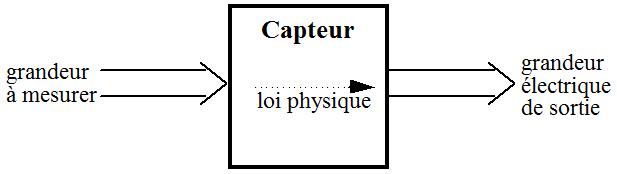
\includegraphics[width=0.96\textwidth]{assets/figures/1_2_Loi_Physique.png}
   \caption{Capteur idéal}
   \label{fig:Loi_Physique}
\end{figure}

Malheureusement le capteur étant un élément réel, le comportement de la grandeur de sortie ne peut être décrit par une seule et unique loi physique: Tout irait bien si, dans notre exemple, la déformation du fil n'était due qu'à la pression; en fait des vibrations, ou une modification de la température peuvent également provoquer une légère déformation du fil, donc une variation non désirée de la résistance; plus grave encore, la température provoque directement une variation de la résistance, indépendante de la déformation et décrite par une autre loi physique.
\begin{figure}
   \centering
   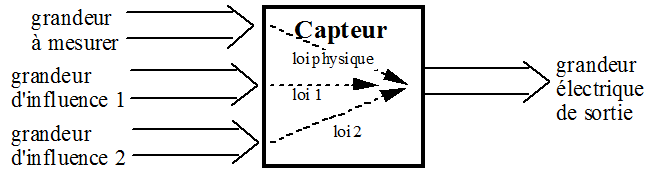
\includegraphics[width=0.96\textwidth]{assets/figures/1_3_Grandeur_Influence.png}
   \caption{Capteur réel}
   \label{fig:Grandeur_Influence}
\end{figure}

Il faut donc bien admettre qu'un capteur n'est jamais idéal, et qu'il doit être représenté par une combinaison de lois physiques, reliant la grandeur de sortie à différentes grandeurs d'entrées. L'une d'entre elles est la grandeur que l'on désire mesurer, appelée le \textbf{mesurande}, les autres sont des \textbf{grandeurs d'influence} car elles modifient la sortie et nous font croire à une variation de la grandeur désirée: le résultat de mesure est influencé par ces grandeurs.
\begin{center}
\fbox{
\begin{minipage}{0.96\textwidth}
\textbf{\textit{Déf}. Grandeurs d'influence Zi :}
toutes les grandeurs d'entrée non désirées du système, dont l'effet sera de modifier la grandeur de sortie.
\end{minipage}
}
\end{center}

\begin{itemize}\itemsep1pt
\renewcommand{\labelitemi}{$\bullet$}
\item Les grandeurs d'influence les plus courantes sont~:
\item La température - elle modifie les valeurs des composants électriques (dimensions, résistivité, tension de seuil dans les composants à semi-conducteur ....)
\item les tensions d'alimentation - elles modifient la polarisation des éléments, donc leur caractéristique, et indirectement leur température
\item Le temps - Les éléments vieillissent et se modifient avec le temps, d'où une dérive lente des caractéristiques
\item L'humidité relative - modifie la constante diélectrique des isolants, provoque des courants de fuite
\end{itemize}

%------------------------------------------
\section{Résolution du problème de mesure}
%------------------------------------------

Dans le processeur du système ou de l'appareil de mesure, on ne dispose que de la sortie numérique $Y$ de la chaîne de mesure. Le problème est donc d'estimer la valeur du mesurande, à partir de la sortie $Y$, et de la connaissance de la caractéristique de la chaîne. Sachant que $Y$ dépend non seulement de $X$, mais aussi des tolérances de fabrication, des grandeurs d'influences, du bruit interne dans les éléments de la chaîne, des perturbations ajoutées par l'environnement, ainsi que de l'effet produit par la présence du capteur sur l'objet mesuré, une solution exacte est impossible.

Il convient donc d'établir un modèle mathématique de la chaîne de mesure, valable dans un certain domaine des conditions d'utilisation, et représentant une approximation de la réponse réelle,
\begin{equation}
Y=\mathcal{F}(X)
\end{equation}
L'opération mathématique inverse ne nous donnera qu'une estimation de la valeur du mesurande,
\begin{equation}
X_m=\mathcal{F}^{-1}(Y)
\end{equation}

\begin{center}
\fbox{
\begin{minipage}{0.96\textwidth}
\textbf{\textit{Déf}. Vraie valeur $X$~:} Valeur du mesurande, qu'on ne connaîtra jamais exactement.
\end{minipage}
}
\end{center}

\begin{center}
\fbox{
\begin{minipage}{0.96\textwidth}
\textbf{\textit{Déf}. Valeur mesurée $X_m$~:} Valeur indiquée par l'appareil de mesure, estimation de $X$.
\end{minipage}
}
\end{center}
Le fabricant d'un instrument de mesure ne peut spécifier l'incertitude de son appareil que pour un domaine bien défini des grandeurs d'influence, et en l'absence de perturbations externes.

Une fois qu'on a obtenu une estimation $X_m$ du mesurande, il reste à déterminer quelle confiance on peut accorder à ce résultat. C'est là tout le problème de l'analyse des mesures.
\begin{center}
\fbox{
\begin{minipage}{0.96\textwidth}
\textbf{\textit{Déf}. Validité des mesures~:}
Degré de confiance que l'on peut accorder au résultat chiffré de la mesure.
\end{minipage}
}
\end{center}

En d'autres termes il s'agit de déterminer si l'on mesure vraiment ce que l'on désire, et d'analyser les causes d'erreurs qui peuvent influencer le résultat. Quelque soit l'équipement utilisé, la méthode d'analyse permettant de répondre à ces questions restera la même, alors que le choix proprement dit de la méthode et des appareils exige une connaissance plus détaillée des principes de mesure de la grandeur concernée.

A titre d'exemple, prenons un capteur de température dans une buse d'injection de PVC (fabrication de pièces injectées), réalisé au moyen d'un thermocouple. Si le montage est parfait, la température indiquée est celle du thermocouple, reste à savoir s'il s'agit bien de la température que l'on désire mesurer : pour éviter l'usure, il faut monter le capteur dans la paroi de la buse d'injection. Quelle est l'influence des échanges thermiques entre la masse à injecter, les parois de la buse et le thermocouple ? De plus le signal électrique fourni par le capteur est de l'ordre de quelques millivolts, et dépend de la température ambiante. L'appareillage tient-il correctement compte de la température ambiante ?  Les moteurs utilisés dans l'équipement d'injection ne rayonnent-ils pas suffisamment de champ électrique et magnétique pour induire une tension parasite s'ajoutant au signal du thermocouple ? La validité des mesures dépendra des réponses à toutes ces questions.

L'exemple ci-dessus nous montre qu'en plus de l'incertitude de l'instrumentation l'analyse de la validité des mesures doit tenir compte des interactions du système de mesure avec l'objet que l'on veut mesurer ainsi qu'avec tout son environnement.

\newpage
L'analyse de la validité des mesures consiste à vérifier l'ordre de grandeur des différentes causes d'erreur:
\begin{itemize}\itemsep1pt
\renewcommand{\labelitemi}{$\bullet$}
\item modèle mathématique (non-conformité, ou non-linéarité)
\item effet des grandeurs d'influence (modification du comportement de la chaîne)
\item bruit interne (limite de détection)
\item perturbations provoquées par l'environnement externe (compatibilité électromagnétique)
\item effet de charge (échange d'énergie entre l'objet mesuré et la chaîne de mesure)
\end{itemize}

%------------------------------------------
\section{Modèle mathématique}
%------------------------------------------

Du fait des fluctuations possibles de la fonction $\mathcal{F}(X)$, les fabricants se contentent de spécifier une approximation mathématique aussi simple que possible à résoudre. Cette approximation ne sera bien sûr pas valable quelle que soit la valeur du mesurande, mais elle se limite à un intervalle bien précis, appelé \textbf{étendue de mesure}.
\begin{center}
\fbox{
\begin{minipage}{0.96\textwidth}
\textbf{\textit{Déf}. Etendue de mesure:}
Domaine des valeurs du mesurande dans lequel le modèle mathématique est valable. En d'autres termes c'est le domaine du mesurande pour lequel le fabricant peut garantir l'incertitude de mesure.
\end{minipage}
}
\end{center}
Bien entendu, l'étendue de mesure sera toujours limitée. Au-delà, soit la sortie diverge, soit elle sature. Par exemple sur un simple amplificateur, lorsque la sortie s'approche de la tension d'alimentation, une saturation intervient.

%------------------------------------------
\section{Forme linéaire, ou linéarisation du modèle de la chaîne de mesure}
%------------------------------------------

C'est la forme mathématique que l'on retrouve dans la grande majorité des cas. En effet, quelque soit la forme de $\mathcal{F}(X)$, pour une étendue de mesure suffisamment faible il est toujours possible de remplacer la courbe $\mathcal{F}(X)$ par un segment de droite. Nous l'écrirons
\begin{equation}
Y = G\cdot X + O
\end{equation}
où le facteur de multiplication $G$ est le \textbf{gain} linéaire de la chaîne de mesure, et $O$ est l'offset, extrapolation de $Y$ en $X=0$.

%------------------------------------------
\section{Forme polynomiale du modèle de la chaîne de mesure}
%------------------------------------------

Lorsque l'étendue de mesure désirée ne permet plus une approximation linéaire, on utilise souvent un polynôme de degré $n$~:
\begin{equation}
Y = a_0 + a_1\cdot X + a_2\cdot X^2 + ... + a_n \cdot X^n
\end{equation}
La forme générale de la réponse est donnée par les $n+1$ coefficients $a_0$ à $a_n$. Ceux-ci sont en général imposés par le type de capteur plutôt que par la chaîne de mesure, mais en général, dans la chaîne, au moins un amplificateur permet d'ajuster tant le décalage $a_0$, qu'un gain global, facteur de multiplication des coefficients $a_1$ à $a_n$.

La résolution du problème de mesure implique l'inversion de la fonction, ce qui revient à utiliser un autre polynôme de degré n exprimant X en fonction de Y ; c'est souvent ce polynôme qui est recherché par régression mathématique :
\begin{equation}
X_m = c_0 + c_1\cdot Y + c_2\cdot Y^2 + .... + c_n\cdot Y^n
\end{equation}

\paragraph{Exemple de modèle quadratique~: capteur de débit à déprimogène}

En plaçant un obstacle dans un fluide dont on désire mesurer le débit (constitué d'un diaphragme, d'un tube Venturi, Pitot ou autre), on provoque localement une différence de pression proportionnelle au carré de la vitesse du fluide à mesurer (loi de Bernoulli, $\Delta p=a_2v^2$). En mesurant la perte de pression, on peut donc mesurer la vitesse du fluide, et partant, son débit, si le fluide est pare exemple confiné dans un tube. En pratique, cependant, $a_2$ ne peut être considéré comme constant que pour une étendue de mesure assez limitée~: débits variant dans un rapport 1 à 3 seulement, car d'autres lois interviennent (détente adiabatique, frottements, turbulence etc.)

\paragraph{Exemple de modèle polynomial à degré élevé~: mesure de température par thermocouple}

Un thermocouple (TC) est la combinaison de 2 conducteurs de matériau différents A et B. La jonction chaude (ou soudure chaude, dont on veut mesurer la température) est le point de contact entre A et B. Les jonctions froides (ou soudures froides) sont les liaisons de A et B avec le circuit de mesure (fils de cuivre). Elles sont en principe à la température ambiante.

La tension que le TC produit est uniquement fonction des températures des jonctions chaude et froides, et est de l'ordre de 5 à 50 $\mu$V/$\degree C$ selon les types de matériaux. Les fabricants fournissent des tables indiquant degré par degré la tension produite lorsque les jonctions froides sont à 0$\degree$C. Puisque ces dernières sont, en pratique, à la température ambiante, il est indispensable de prévoir une correction.
%La théorie de la thermoélectricité nous indique que la tension indiquée dans les tables est égale à la somme de la tension produite UTC lorsque les jonctions froides sont à une température différente de zéro et de la tension indiquée dans les tables des fabricants à la température des jonctions froides Utable(Tfr):
%\begin{equation}
%\mathcal{U}_{table}(T_{ch}) = \mathcal{U}_{TC} + \mathcal{U}_{table}(T_{fr})
%\end{equation}
%Le circuit de mesure doit donc non seulement mesurer UTC, mais également la température des jonctions froides $T_{fr}$ (au moyen d'un $2^e$ capteur). La résolution du problème de mesure consiste d'une part à retrouver $U_{table}(T_{fr}$) pour permettre le calcul de $U_{table}(T_{ch}$), puis à calculer $T_ch$ à partir de $U_{table}(T_{ch})$.
Pour de grands domaines de températures, cette opération exige d'utiliser, pour le modèle, un polynôme du 9ème degré.
%, alors que pour la compensation de jonction froide le domaine 0 à 50  $\degree$ C est suffisant et peut être approché par un polynôme du $2^e$ degré seulement.

%------------------------------------------
\section{Loi physique du capteur}
%------------------------------------------
Enfin, plus rarement, le modèle découle directement de la loi physique exploitée dans le capteur, si besoin corrigée et complétée par des termes de type expérimental.

\paragraph{Exemple : Mesure de température par thermistance}

Une thermistance est une résistance en mode semi-conducteur, dont la valeur varie avec la température, selon
\begin{equation}
R(T) = R_{25}\exp{\left[b\left(\frac{1}{T}-\frac{1}{298}\right)\right]}
\end{equation}
où $T$ est en kelvin, $R_{25}$ est la résistance à 25$\degree$C, c-à-d 298$\degree$K, et $b$ un coefficient (en kelvin) caractéristique du semi-conducteur. En inversant la fonction on trouve~:
\begin{equation}
\frac{1}{T} = \frac{1}{b}\ln{\left(\frac{R}{R_{25}}\right)}+\frac{1}{298} = A + B\,\ln{R}
\end{equation}
L'expérience montre cependant que le coefficient $b$ ne peut être considéré comme constant que dans un faible domaine de température (15 à 25$\degree$C), par conséquent l'équation ci-dessus a été complétée (à la manière polynomiale) suivant
\begin{equation}
\frac{1}{T} = A + B \ln{R} + C \ln^3{R}
\end{equation}
Cette expression est alors valable dans un domaine de 100 à 150$\degree$C avec une incertitude de l'ordre de 0.01$\degree$ C.

%------------------------------------------
\section{Erreurs de non conformité ou de non-linéarité}
%------------------------------------------

A l'intérieur du domaine de mesure, le modèle mathématique ne fait que s'approcher et lisser la réponse réelle. Ceci conduit à des erreurs que l'on appelle de manière générale erreurs de non-conformité, ou de non-linéarité dans le cas d'un modèle linéaire. Ces notions seront traités dans le chapitre 4.

%------------------------------------------
\section{Bruit interne}
%------------------------------------------

La conduction électrique se faisant par déplacement de charges électriques élémentaires, le signal de sortie ne peut être rigoureusement constant même si les conditions d'utilisation ne changent pas. On constate l'addition d'un petit signal aléatoire à l'information souhaitée : c'est le bruit interne d'agitation thermique dans les résistances, ou le bruit de grenaille typique dans les jonctions de semi-conducteur. Si ces bruits sont généralement négligeables, ils représentent cependant la limite absolue de détection du circuit~: en effet, pour pouvoir distinguer une variation du signal, il faut que celle-ci soit significativement plus grande que la fluctuation aléatoire du bruit interne du système.

%------------------------------------------
\section{Grandeurs d'influence}
%------------------------------------------

Comme déjà indiqué, la grandeur de sortie d'un capteur dépend non seulement du mesurande, mais également d'autres grandeurs physiques, comme la température par exemple. Ces autres grandeurs physiques sont appelées grandeurs d'influence.

La spécification d'incertitude, donnée par le fabricant, tient compte du bruit interne ainsi que des grandeurs d'influences, dans un domaine particulier, qu'il se doit d'indiquer dans les spécifications, par exemple $23\pm5^\circ$C, alimentation 220 V$\pm$10\%.

Le rôle de l'opérateur est donc d'abord de vérifier que les grandeurs d'influence sont bien à l'intérieur du domaine prévu par le constructeur, au moment où l'on effectue les mesures. Ensuite seulement, il pourra utiliser l'incertitude comme critère de validité. Lorsque les grandeurs d'influence sortent des domaines d'utilisation prévus, il convient de tenir compte des coefficients d'influence, ou de calibrer l'instrumentation.

%------------------------------------------
\section{Effet de charge}
%------------------------------------------

L'interaction entre l'objet à mesurer et le système de mesure exige un transfert d'énergie, si petit soit-il. La présence du capteur, et du système de mesure va donc un tant soit peu modifier l'état du processus que l'on cherche à observer. Il devient donc impossible de connaître l'état qu'aurait le processus en l'absence du système de mesure, mais en choisissant correctement le capteur et le système, on peut minimiser ces effets, et s'approcher de la \textless\textless\ vraie\ \textgreater\textgreater valeur qu'aurait le processus \textless\textless\ à vide\ \textgreater\textgreater.

Le transfert d'énergie, n'est pas la seule cause d'effet de charge~: pour pouvoir insérer le capteur à l'endroit de la mesure, il faut généralement modifier la structure de l'objet, donc en modifier le comportement. La difficulté est alors de choisir un capteur et un lieu de mesure permettant d'éviter trop de modifications du comportement du processus, tout en maintenant la possibilité d'obtenir des mesures significatives.
\begin{center}
\fbox{
\begin{minipage}{0.96\textwidth}
\textbf{\textit{Déf}. Effet de charge (loading effect) :}
Modification de l'état du processus et du système de mesure dû aux sorties non désirées du transducteur (échange d'énergie) ou au changement de structure  du processus imposé par la présence du transducteur.
\end{minipage}
}
\end{center}

\paragraph{Exemples}

\begin{enumerate}
\item Un voltmètre a toujours une résistance interne $R_v$. La mesure de la tension de charge $U_b$ d'une batterie de résistance interne $R_i$ s'accompagne du passage d'un courant $i = U_b/(R_i+R_v)$. La puissance transférée au voltmètre est donc $P=U_v\cdot i$. L'effet de charge se traduit donc par le fait que le voltmètre ne mesure pas exactement $U_b$, mais
\begin{equation}
U_v=U_b\cdot\frac{R_v}{R_v+R_i}
\end{equation}
\item Pour mesurer la résistance d'une jauge de contrainte, il faut faire passer un courant dans le fil. Ce courant provoque un échauffement du capteur, qui se transmet au support et conduit à une modification de la grandeur d'influence (la température), donc de la grandeur de sortie. Il y a  effet de charge par échange d'énergie. De plus, le fait de coller la jauge sur son support modifie la constante d'élasticité locale. Pour une même contrainte, la déformation sera légèrement différente: c'est un 2e effet de charge dû à une modification de structure du processus.
\item Pour mesurer la vitesse des gaz à la sortie d'une tuyère, il faut placer une sonde, dans le flux de gaz. Aussi petite que soit la sonde, elle va modifier les lignes de flux. Il y a effet de charge par modification structurelle.
\end{enumerate}

L'effet de charge se traduit par une erreur systématique (= elle se produit toujours dans le même sens: addition d'une petite constante ou multiplication de la valeur mesurée par un facteur proche de l'unité). C'est donc lors de la conception du système de mesure que l'opérateur doit analyser cet effet, et sélectionner une instrumentation adaptée à l'objet mesuré. A noter que puisque l'erreur due à l'effet de charge est systématique, il est possible de la corriger, ce qui est un avantage par rapport aux erreurs de type aléatoires, imprédictibles par nature.

\newpage

%------------------------------------------
\section{Perturbations}
%------------------------------------------

Le fait que les équipements de mesure et de contrôle sont placés dans un environnement naturel les soumet à des perturbations : rayonnements cosmiques, éclairs dans un orage, bruit intrinsèque dans la matière même des éléments. De plus l'activité humaine est également source de perturbations : émission radio et TV, communications haute fréquence, champs électromagnétiques des lignes de distribution d'énergie, des moteurs et générateurs, étincelles d'allumage des moteurs à combustion etc. Dans un appareillage électrique, ces perturbations sont couplées par les champs électromagnétiques dans les circuits, ce qui se traduit par une tension ou un courant perturbateur s'ajoutant au signal sur la grandeur de sortie.

L'appareillage doit répondre à des normes de compatibilité électrique, assurant qu'il n'est pas perturbé par des champs externes, et qu'il n'émet pas trop de perturbations. Par ailleurs le câblage entre appareils peut fort bien fonctionner comme antenne, et introduire des perturbations dans le système de mesure.

Il existe des méthodes pour se protéger contre de telles perturbations, essentiellement par le choix du câblage, du type d'amplificateur, et des méthodes de transmission du signal. Lors de l'analyse de validité, il convient de détecter la présence et l'ordre de grandeur des perturbations. Ceci implique une analyse du signal de sortie, soit sous la forme temporelle mais le plus souvent dans le domaine fréquentiel (détection d'une composante alternative non liée au mesurande).

%------------------------------------------
\section{Systèmes d'acquisition de données}
%------------------------------------------

\begin{center}
\fbox{
\begin{minipage}{0.96\textwidth}
\textbf{\textit{Déf}. Système d'acquisition de données :}
tout ensemble d'appareils interconnectés de manière à permettre l'obtention automatique d'une série de mesure sur un objet. Ce dernier peut aller d'un simple circuit intégré à une chaîne de fabrication complète.
\end{minipage}
}
\end{center}
L'analyse et le choix des caractéristiques du système de mesure étant fortement liés à l'application, il est clair qu'il n'est pas possible d'énoncer des règles universelles. L'objectif de ce paragraphe est cependant de donner une vision générale de ces systèmes et de leurs composants. Le choix d'une réalisation doit être le résultat d'un travail de synthèse entre les connaissances des moyens de mesure, des structures possibles et des éléments disponibles.

\begin{figure}[h]
\centering
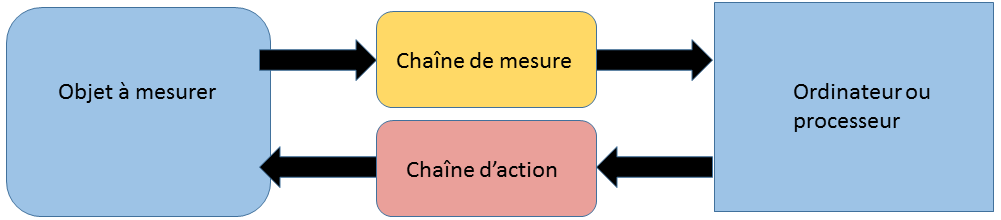
\includegraphics[width=0.9\textwidth]{assets/figures/fig_TechMes_CBD_SysTypdAcquDeDonnees.png}
\caption{Système typique d'acquisition de donnees}
\label{fig:SystemeTypiquedAcquisitionDeDonnees}
\end{figure}

Tout système d'acquisition comprend au moins une chaîne de mesure. Dès que l'on est en présence de plusieurs chaînes, se pose la question d'une économie de matériel en exploitant un multiplexage, soit sous forme analogique (sortie des conditionneurs ou transmetteurs connectées successivement à un seul convertisseur A/D), soit sous forme numérique (les convertisseurs sont reliés à l'ordinateur au travers d'un bus numérique).

Dans la majorité des cas, il faut pouvoir agir sur l'objet mesuré au moyen de chaînes d'action. L'action recherchée peut être de type tout ou rien (arrêt d'urgence, enclenchement - déclenchement d'une pompe ou d'un chauffage...) ou de type analogique (envoi d'un stimulus, commande d'une vanne proportionnelle, de la vitesse d'un moteur ...). Dans le premier cas un signal logique de sortie de l'ordinateur commande un relais permettant d'appliquer ou non une puissance fixe sur l'actionneur. Dans le second cas la chaîne d'action comprend un convertisseur digital - analogique (D/A) qui commande l'actionneur au travers d'amplificateurs de puissance.

Le coeur du système est son ordinateur ou processeur, chargé de commander la séquence de travail, d'effectuer les calculs nécessaires au traitement numérique, d'assurer le sauvetage et la transmission des données ainsi que de la communication avec l'opérateur du système. Selon le type d'application on peut se contenter d'un simple microcontrôleur, exploiter un processeur de calcul numérique (DSP) ou devoir exploiter un ordinateur haut de gamme.

\begin{figure}[p]
    \centering
	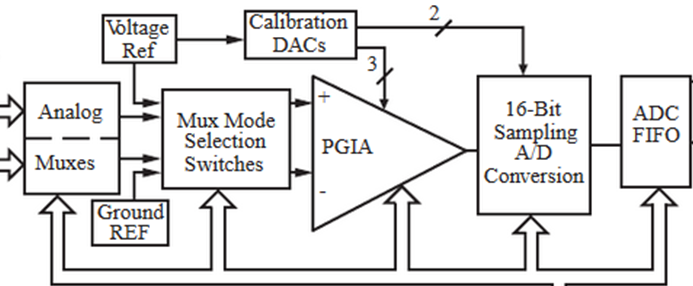
\includegraphics[width=0.9\textwidth]{assets/figures/2_9a_Analog_Frontend.PNG}
	\caption{Carte universelle d'acquisition: entrées analogiques.}
	\label{fig:Analog_Frontend}
	\vspace{5mm}
    \centering
	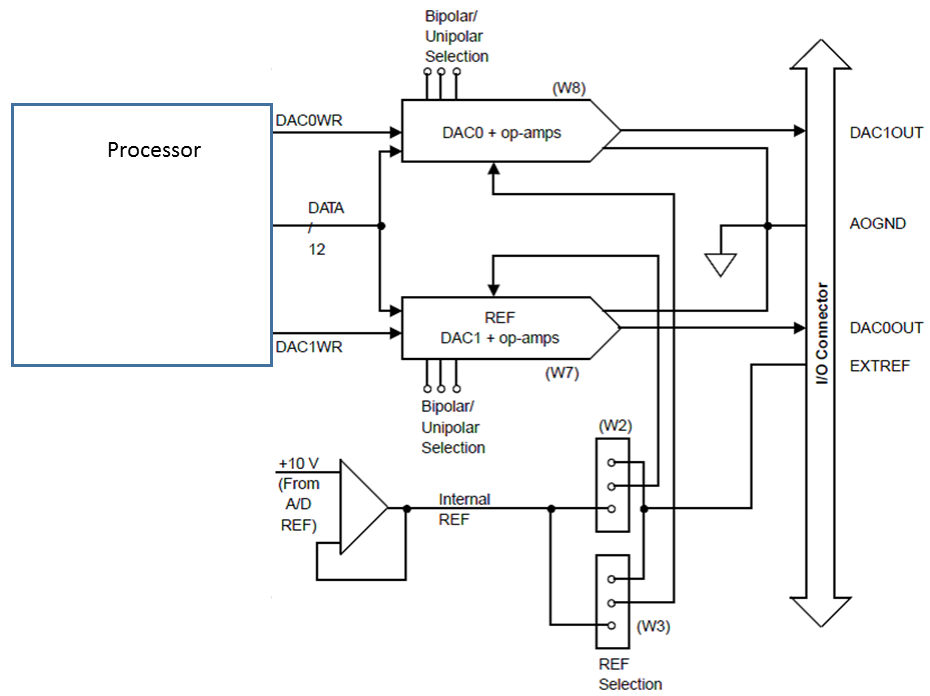
\includegraphics[width=0.9\textwidth]{assets/figures/2_9b_Sorties_analogiques.PNG}
	\caption{Carte universelle d'acquisition: sorties analogiques.}
	\label{fig:Sorties_analogiques}
\end{figure}

%------------------------------------------
\section{Architectures}
%------------------------------------------

Les cartes universelles d'acquisition permettent de réaliser à bon marché des applications d'acquisition et de contrôle de processus. Il ne faut pas oublier cependant que leur résolution et leur précision sont limitées, qu'elles sont sujettes à passablement de bruit (terre de l'ordinateur largement perturbée par les transitoires de la logique rapide) et que les fréquences d'échantillonnage sont limitées tant par le nombre de canaux à mesurer que par la nécessité de les commander directement par le processeur.

Les figures ~\ref{fig:Analog_Frontend} et ~\ref{fig:Sorties_analogiques} présentent une architecture de carte d'acquisition universelle. On constate que l'entrée analogique est formée de 2 multiplexeurs et non d'un seul. Cela permet d'effectuer des mesures différentielles, dans le but d'éliminer les perturbations communes aux deux fils de connexion, à savoir le signal et sa référence si la liaison est asymétrique, ou le signal positif et le signal négatif si la transmission est différentielle. On notera que sur chacun des cas d'entrée ou de sortie, une référence de tension est présente. Sa précision et sa stabilité sont essentielles pour garantir la qualité des mesures.

%------------------------------------------
\section{Modes du multiplexeur}
%------------------------------------------

Trois modes de fonctionnement du multiplexeur analogique sont à disposition:

\begin{itemize}\itemsep1pt
\renewcommand{\labelitemi}{$\bullet$}
\item SE - Asymétrique: Fig.~\ref{fig:Mesure_asymetrique}. Le multiplexeur relie l'une des 16 bornes d'entrée (Ain0 à Ain15) à l'entrée \textless\textless\ hi \ \textgreater\textgreater du PGA, alors que l'entrée \textless\textless\ lo \ \textgreater\textgreater est mise à la masse (gnd) de la carte. On mesure ainsi le potentiel de la borne correspondante par rapport  à la carte. Cette méthode est donc dangereuse, si les sources de signal sont référées à la masse locale : le bruit au niveau de la masse du pc s'ajoute aux signaux mesurés. A n'utiliser que pour des sources de signal flottantes dont on pourra connecter la borne de référence à la masse de la carte !!
\item RSE - pseudo-différentiel ou asymétrique à référence externe : Fig.~\ref{fig:Mesure_Pseudo_differentielle}. le multiplexeur fonctionne de la même manière, mais la borne \textless\textless\ lo \ \textgreater\textgreater du PGA est reliée à la borne \textless\textless\ Aisense \ \textgreater\textgreater du connecteur externe. Il faut alors relier cette borne à la référence zéro (généralement la masse) de l'objet à mesurer. On élimine ainsi les problèmes de bruit au niveau de la masse du PC. Cependant toutes les sources de signal doivent être reliées à ce même point commun \textless\textless\ Aisense \ \textgreater\textgreater.
\item Diff - Vrai différentiel : Fig.~\ref{fig:Mesure_differentielle}. le multiplexeur est séparé en deux parties travaillant simultanément : la partie A relie le canal i (Ain0 à Ain7) à la borne \textless\textless\ hi \ \textgreater\textgreater, pendant que la partie B relie la borne correspondante i+8 (Ain8 à Ain15) à la borne \textless\textless\ lo \ \textgreater\textgreater. On mesure alors vraiment la différence de potentiel entre un couple de bornes (Ain0 et Ain8, Ain1 et Ain9 ...), mais on ne dispose plus que de 8 canaux. La seule exigence à respecter est que le mode commun reste dans le domaine supporté par le PGA, soit que chacune des bornes reste dans le domaine de $\pm$ 11V par rapport à A-gnd (masse de la carte).
\end{itemize}

\begin{figure}[p]
    \centering
    \vspace{-17mm}
	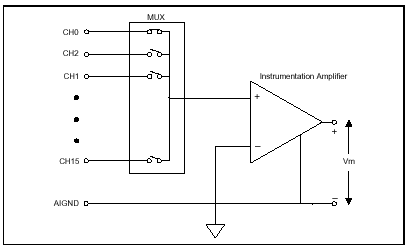
\includegraphics[width=10cm]{assets/figures/2_10_Mesure_asymetrique.PNG}
	\caption{Mesure asymétrique (SE = Single Ended).}
	\label{fig:Mesure_asymetrique}
    \centering
	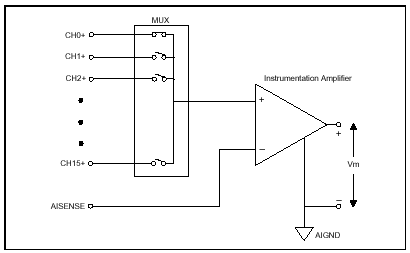
\includegraphics[width=10cm]{assets/figures/2_11_Mesure_Pseudo_differentielle.PNG}
	\caption{Mesure Pseudo-différentielle ou Asymétrique référencée (RSE = Referenced Single Ended).}
	\label{fig:Mesure_Pseudo_differentielle}
    \centering
	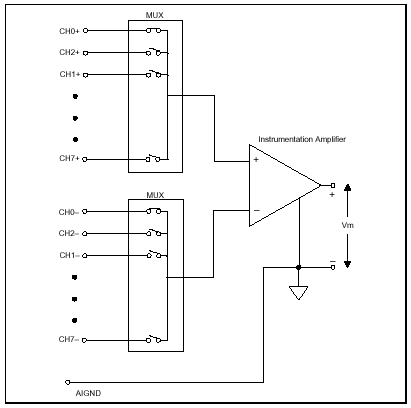
\includegraphics[width=10cm]{assets/figures/2_12_Mesure_differentielle.PNG}
	\caption{Mesure différentielle.}
	\label{fig:Mesure_differentielle}
\end{figure}

\newpage
%------------------------------------------
\section{Sources flottantes et courants de polarisation}
%------------------------------------------

Lorsqu'on mesure une source flottante, il faut prévoir un chemin de retour vers A-gnd pour les courants de polarisation du PGA (mode RSE et Diff). L'absence d'un tel chemin galvanique provoquerait la saturation du PGA. Ces courants sont inférieurs à 200 pA. Une résistance de l'ordre de 100 kOhms contre A-gnd, suffit, mais afin de ne pas dégrader le taux de réjection du mode commun, il est préférable de connecter une résistance sur chacune des deux entrées (hi et lo). Le dimensionnement de ces résistance se fait en fonction du mode commun : ce montage ajoute un mode commun de (200 pA*100kOhms) = 20 uV généralement négligeable. On voit qu'on pourrait sans autre fortement augmenter la valeur des résistances.

%------------------------------------------
\section{Conditionnement des signaux}
%------------------------------------------

Bien que le fait de disposer d'un PGA permette un grand choix des gammes de mesures (100mV à 10V en unipolaire et +/-50mV à +/-10V en bipolaire), la plupart des applications exigent d'utiliser des circuits de conditionnement  (capteur, atténuateur, amplificateur, shunt ...) avant de relier les signaux à la carte. Le pilote de la carte est généralement capable de tenir compte automatiquement du gain du PGA. Il peut ainsi fournir les résultats des conversions selon deux options :
\begin{itemize}\itemsep1pt
\renewcommand{\labelitemi}{$\bullet$}
\item en V au niveau du connecteur d'entrée (nombre réel).
\item ou directement le code de conversion sous forme d'un nombre entier (+/-2048).
\end{itemize}
C'est à l'utilisateur de tenir compte des caractéristiques de conditionnement pour calculer l'équivalent de la grandeur mesurée en unités physique (degrés Celsius, Bar, Kg ...)

%------------------------------------------
\section{Les différents types de signaux}
%------------------------------------------

Un système de mesure transforme une \textbf{entrée}, en règle générale une grandeur physique, en un signal de \textbf{sortie}. Différents types de signaux sont transmis entre les capteurs, les conditionneurs et la sortie du système.

On peut classifier les signaux en trois catégories selon leur représentation temporelle et les valeurs prises par la quantité mesurée (fig.~\ref{fig:typsign1})~:
\begin{description}
\item[Un signal continu] est défini pour toutes les valeurs du temps et peut prendre n'importe quelle valeur en amplitude,
\item[Un signal discret] est en général un signal continu qui est mesuré à certains instants seulement, mais il peut aussi s'agir d'un signal naturellement discontinu, tel que le nombre de photons reçus par un détecteur pendant une certaine durée de temps, un nombre de véhicules par tranche d'heure sur une route, etc.
\item[Un signal numérique] est un signal discret quantifié sur un certain nombre de niveaux (généralement des puissances de 2) et qui ne peut prendre qu'un ensemble discret de valeurs, par exemple la numérisation d'un signal électrique de -10 à +10 V sur 8 bits non signés, de 0 à 255.
\end{description}
\begin{figure}[h]
   \centering
   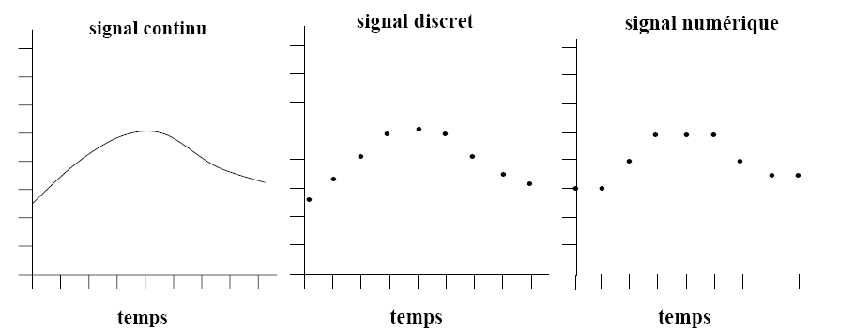
\includegraphics[width=13cm]{assets/figures/typesign.pdf}
   \caption{Les trois types de signaux les plus fréquents.}\vspace{5mm}
   \label{fig:typsign1}
   \centering
   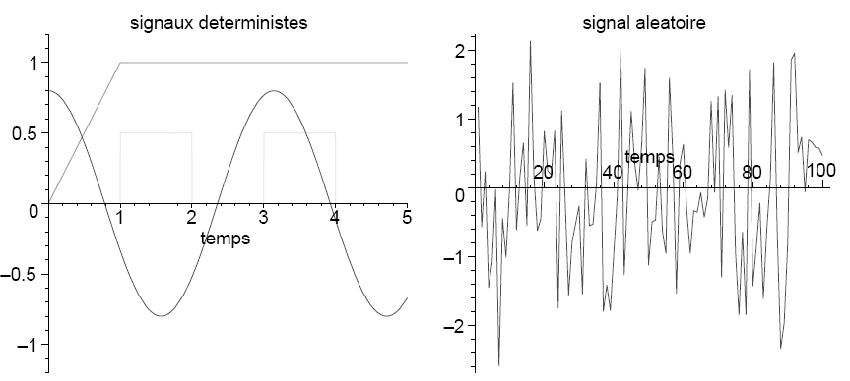
\includegraphics[width=13cm]{assets/figures/sigda.pdf}
   \caption{Signaux déterministes et aléatoires.}
   \label{fig:sigda1}
\end{figure}
En fonction du phénomène physique qu'ils représentent, il faut aussi distinguer les signaux \textbf{déterministes}, c'est-à-dire les signaux pour lesquels les valeurs futures peuvent être prédites, et les signaux \textbf{aléatoires} qui ne sont pas prédictibles et qui nécessitent un traitement spécifique (fig.~\ref{fig:sigda1}).

%------------------------------------------
\section{Exercices}
%------------------------------------------

\subsection{Exercice: Résistances de polarisation}
La carte d'acquisition MIO16 du labo est spécifiée avec une impédance d'entrée de $100G\Omega$ en parallèle avec 50 pF. Le courant de polarisation d'entrée est de $\pm200pA$, et le domaine des tensions d'entrée (signal + mode commun) est de $\pm11V$.

Dimensionner les résistances de polarisation à brancher entre les entrées et la terre A-Gnd de la carte, pour des sources flottantes, dans le cas d'une gamme de mesure de $\pm50mV$, et dans le cas d'une gamme de mesure de $\pm5V$, en mode différentiel.


\subsection{Exercice: Fréquence de scrutation}
La carte d'acquisition MIO16 du labo est spécifiée avec une impédance d'entrée de $100G\Omega$ en parallèle avec 50 pF. Le convertisseur est un 12 bits - 100 kéch/s. On l'utilise pour mesurer 4 canaux dont les impédances de sortie sont de $5k\Omega$. Déterminer s'il faut changer la fréquence de scrutation (critère : établissement à 1 LSB), et quelle est la fréquence maximum d'échantillonnage que l'on pourra obtenir.

\subsection{Exercice: Multiplexage et déphasage}
A l'aide d'une carte 250 kéch/s, on mesure 5 canaux. Calculer quel est le déphasage maximum entre les canaux introduit artificiellement par le multiplexage, en fonction de la fréquence des signaux, ainsi qu'à 1kHz et à 10 kHz.


%%%%%%%%%%%%%%%%%%%%%%%%%%%%%%%%%%%%%%%%%%%%%%%%%%%%%%%%%%%%%%%%%%%%%%%%%%%%%%%%%%%%%%
%%%%%%%%%%%%%%%%%%%%%%%%%%%%%%%%%%%%%%%%%%%%%%%%%%%%%%%%%%%%%%%%%%%%%%%%%%%%%%%%%%%%%%
\chapter{Modélisation de la chaîne}
%------------------------------------------

\begin{figure}[h]
   \centering
   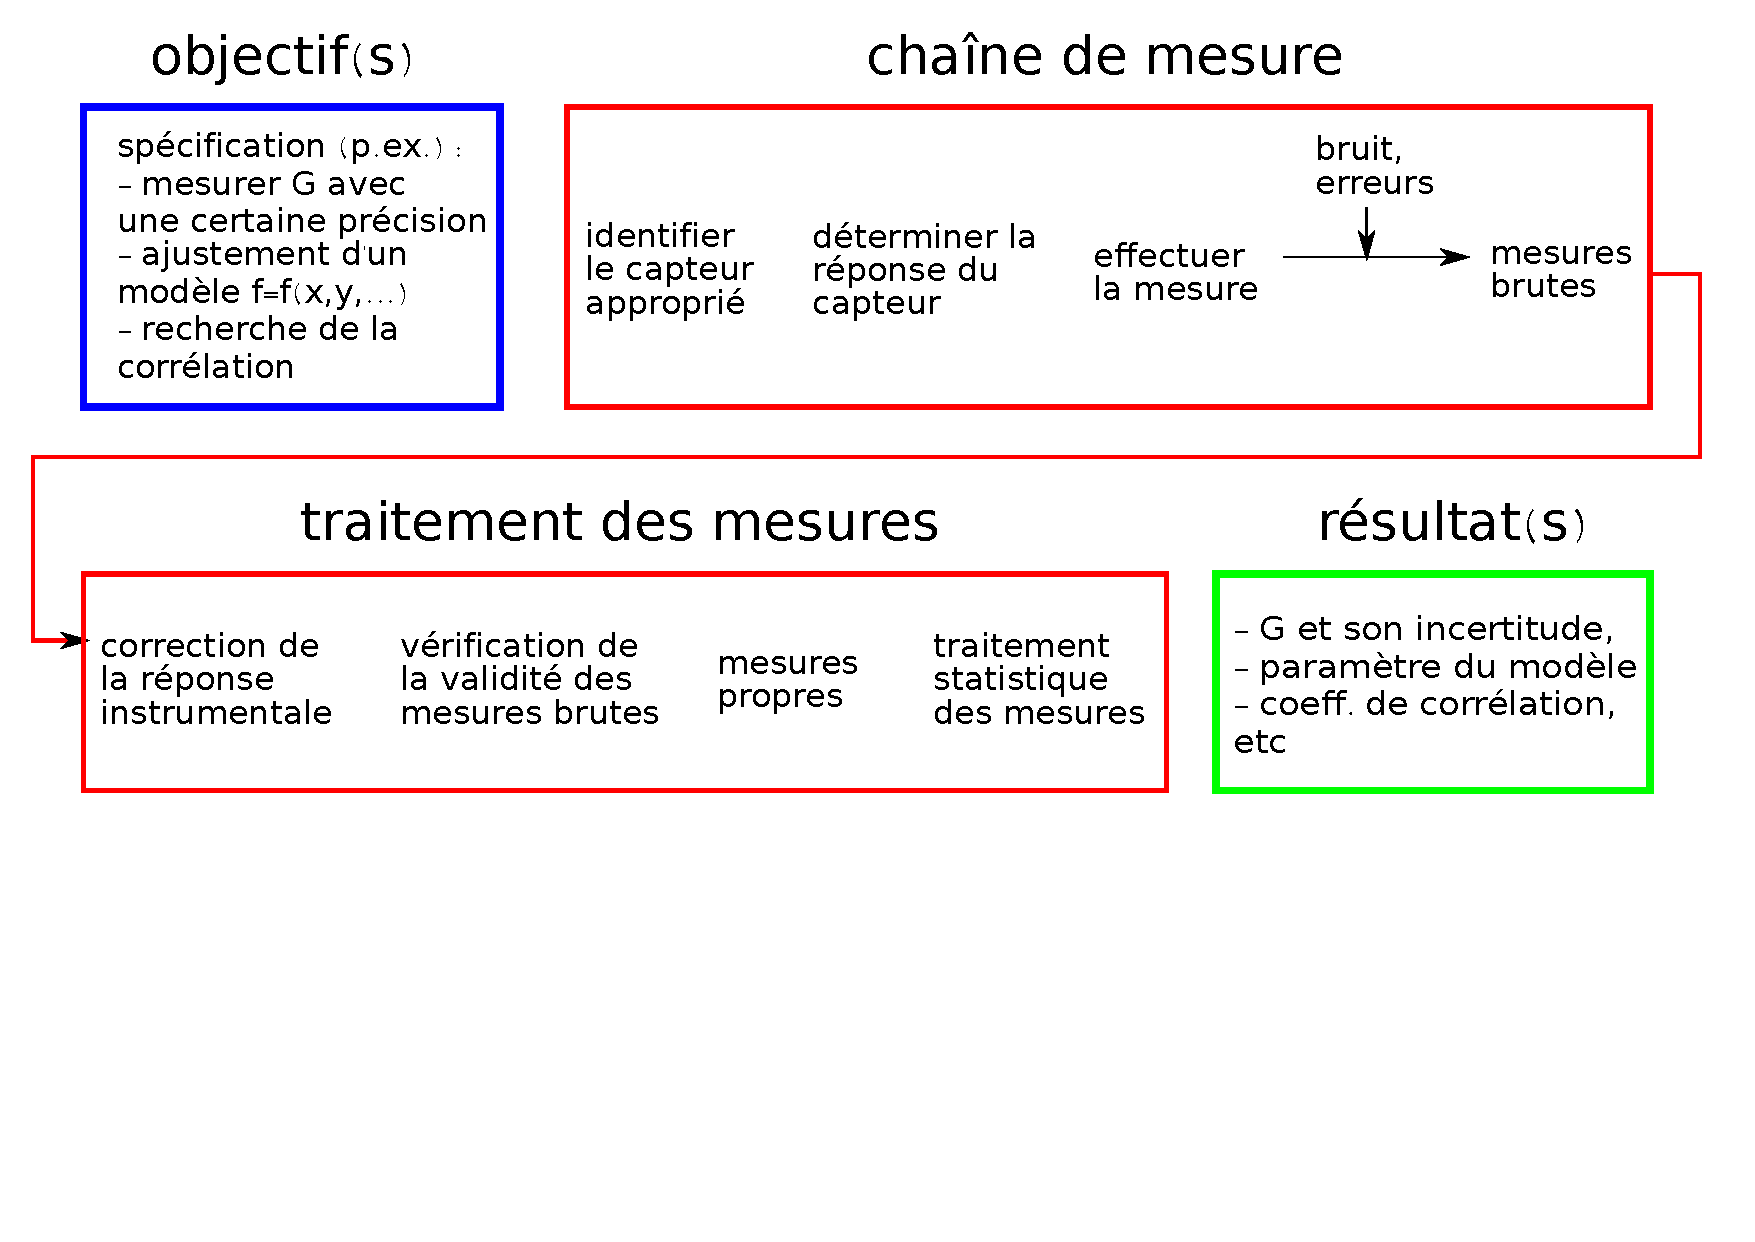
\includegraphics[width=0.96\textwidth]{assets/figures/flowChartTechMes.pdf}
   \caption{Techniques de mesure: étapes clés}
   \label{fig:flowChartTechMes}
\end{figure}

Reprenant le schéma bloc des étapes clé des techniques de mesure, nous souhaiterions aborder le traitement des mesures. Toutefois nos connaissances de la chaîne de mesure sont encore insuffisantes: nous devons maintenant comprendre comment modéliser la chaîne de mesure afin d'avoir les outils et informations nécessaires aux traitements mathématiques qui vont suivre.

Pour résoudre le problème de la mesure, à savoir retrouver la valeur du mesurande à partir de la sortie du capteur, il faut inverser la fonction mathématique F(X) liant le mesurande à la sortie. La difficulté vient du fait que F(X) est mal définie: du bruit s'ajoute au signal de sortie, les grandeurs d'influence modifient la fonction, les tolérances de fabrication conduisent à une fonction réelle légèrement différente de la fonction nominale. De plus les lois physiques qui régissent le capteur et la chaîne de mesure peuvent conduire à une expression mathématique complexe de la fonction.

%------------------------------------------
\section{Approximations mathématiques}
%------------------------------------------

Nous avons vu au chapitre 1 que les approximations mathématiques pouvaient être faites au travers de modèles de formes mathématiques diverses : linéaire, polynomiale ou découlant directement de la loi physique exploitée dans le capteur. Pour la suite de l'analyse, \textbf{nous ne considérerons ici que le cas linéaire.}

%------------------------------------------
\section{Incertitudes}
%------------------------------------------

Le modèle linéaire est une droite, ne passant pas nécessairement par l'origine, approchant au mieux la caractéristique de la chaîne de mesure:
\begin{center}
\fbox{
\textbf{Y = G X  + Of}
}
\end{center}

Cette équation fait intervenir les deux paramètres G et Of, caractéristiques de la chaîne.
\begin{center}
\fbox{
\begin{minipage}{0.96\textwidth}
\textbf{\textit{Déf}. Gain  (G) :}
Pente de la caractéristique entrée-sortie
\\
\\
\textbf{\textit{Déf}. Décalage (Of) :}
Ordonnée à l'origine du modèle linéaire (de l'anglais "offset")
\end{minipage}
}
\end{center}

Il est fondamental de ne jamais oublier qu'il ne s'agit là que d'une approximation de la courbe de réponse (forme de la réponse pas tout à fait droite, tolérances de fabrication), et de plus que cette approximation est variable dans le temps, en raison des grandeurs d'influence (vieillissement, température, ...) ou des conditions d'utilisation (effet de charge, perturbations,...). Le fabricant nous indique les valeurs nominales du gain et du décalage $G_{nom}$ et $Of_{nom}$.
On résout le problème de mesure sur la base de ces valeurs nominales, et l'on obtient alors une estimation $X_{m}$ de la grandeur d'entrée X :
\begin{center}
\fbox{
\begin{minipage}{0.96\textwidth}
\textbf{\textit{Déf}. Erreur absolue (e) :}
Ecart entre la valeur mesurée et la vraie valeur 	$e = X_{m} - X$
\newline
\newline
\textbf{\textit{Déf}. Erreur relative ($\epsilon$) : }
\text{Quotient entre erreur absolue et vraie valeur  }	$\epsilon = \frac{e}{X}  \cong \frac{e}{X_{m}}$
\end{minipage}
}
\end{center}

Pour analyser l'erreur, il faut tenir compte des écarts entre la courbe réelle et son approximation linéaire dans les conditions de mesure, ainsi que du fait que cette approximation diffère légèrement de la droite nominale. Nous écrivons donc une nouvelle expression de la sortie Y
\begin{equation}
Y = G_{reel}X + Of_{reel} + L(X,t)
\end{equation}
où $G_{reel}$ et $Of_{reel}$ représentent le modèle linéaire actuel, tenant compte des grandeurs d'influence et effets de charge. $L(X,t)$ représente l'écart entre la courbe et la droite du modèle actuel, ainsi que le bruit ajouté à la sortie. On ne connaît jamais ces trois termes, mais un étalonnage dans des conditions données des grandeurs d'influence permet au fabricant de spécifier les écarts maximum. Exprimons l'erreur:
\begin{gather}
e = X_m - X =  Y - \frac{Of_{nom}}{G_{nom}} - X = \frac{G_{reel}X + Of_{reel} + L -Of_{nom}}{G_{nom}} - X\\
e = X \cdot(\frac{G_{reel}}{G_{nom}}   - 1) +  \frac{Of_{reel} - Of_{nom}}{G_{nom}}   +  \frac{L}{G_{nom}}
\end{gather}
c-à-d
\begin{equation}
e = X \cdot \alpha  + D + NL
\end{equation}
On constate alors que l'erreur est la somme de trois termes. Les deux premiers expriment des erreurs systématiques fonctions des grandeurs d'influence (dérive du modèle linéaire par rapport aux valeurs nominales), le troisième peut être assimilé à une erreur aléatoire.
\begin{center}
\fbox{
\begin{minipage}{0.95\textwidth}
\textbf{\textit{Déf}. Erreur de gain  ($\alpha$) :}\\
Erreur relative du gain de la chaîne: Gréel - GnomGnom  .  Correspond à une rotation de la courbe autour de l'origine. Provoque une erreur systématique proportionnelle au mesurande (calculable seulement si l'on connaît toutes les grandeurs d'influence)\\
\\
\textbf{\textit{Déf}. Erreur de décalage (D) :}\\
Erreur absolue à l'origine: Ofréel - OfnomGnom  . Correspond à une translation verticale de la courbe de réponse. Provoque une erreur systématique constante, indépendante de X (calculable seulement si l'on connaît toutes les grandeurs d'influence)\\
\\
\textbf{\textit{Déf}. Erreur de non-linéarité (NL)}\\
Ecart entre la droite du modèle actuel et la courbe réelle de réponse. Fonction du mesurande, si bien qu'on la considère comme une grandeur aléatoire.
\end{minipage}
}
\end{center}
Le fabricant indique l'incertitude de la chaîne ou d'un appareil en combinant ces trois erreurs et le bruit interne.

\begin{center}
\fbox{
\begin{minipage}{0.96\textwidth}
\textbf{\textit{Déf}. Incertitude de mesure :	}
Valeur limite que peut prendre l'erreur (en valeur absolue), avec un certain degré de confiance, en général 99 \%. En d'autres termes, si l'on a spécifié une incertitude I, la valeur absolue de l'erreur e sera dans 99 \% des cas inférieure à I : 	|e| < I 	(99 fois sur 100)
\end{minipage}
}
\end{center}

\begin{figure}
\centering
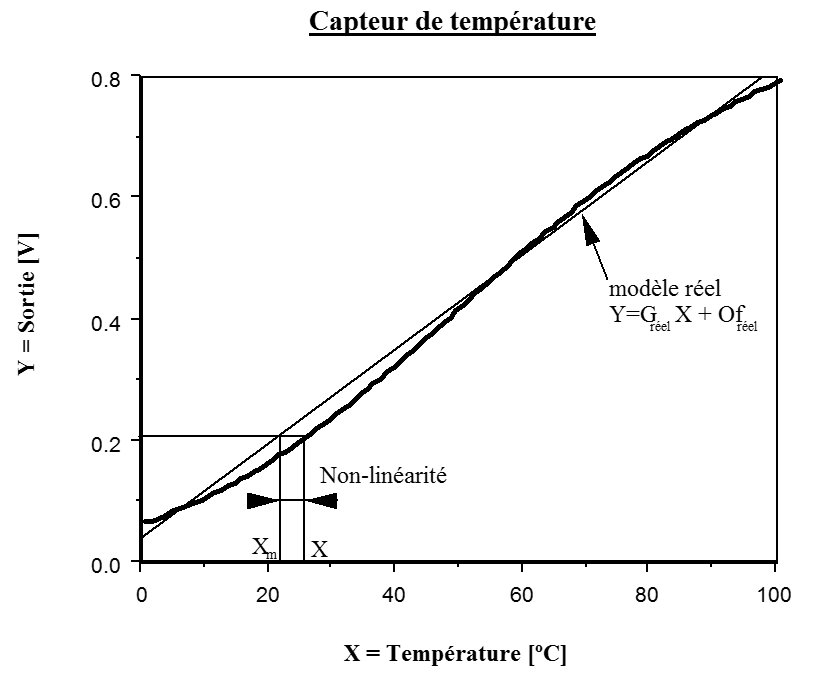
\includegraphics[height=8cm]{assets/figures/3_1_Non_Linearite.PNG}
\caption{Non-linéarité.}
\label{fig:Non-linéarité}
\end{figure}
La spécification de l'incertitude comprend deux termes, pour tenir compte du fait que l'une des composantes est proportionnelle à X. L'erreur de gain est toujours spécifiée sous forme d'une valeur relative $\alpha$ (en \%, \textperthousand ~ ou ppm, soit des facteurs de $10^{-2}, 10^{-3}, ou 10^{-6}$), alors que l'effet global du décalage, des non-linéarités et du bruit interne est spécifié comme un terme indépendant de X, soit sous forme absolue B (unités de X, ou unités d'affichage: divisions sur un écran analogique, digit sur un affichage numérique), soit sous forme relative $\beta$ par rapport à une grandeur caractéristique de la chaîne: gamme de mesure, étendue de mesure, ou pleine échelle.
\begin{equation}
I = \alpha \cdot \text{lect} + B \cdot digit = \alpha \cdot \text{lect} + \beta \cdot \text{gamme}
\end{equation}

\begin{figure}[h]
\centering
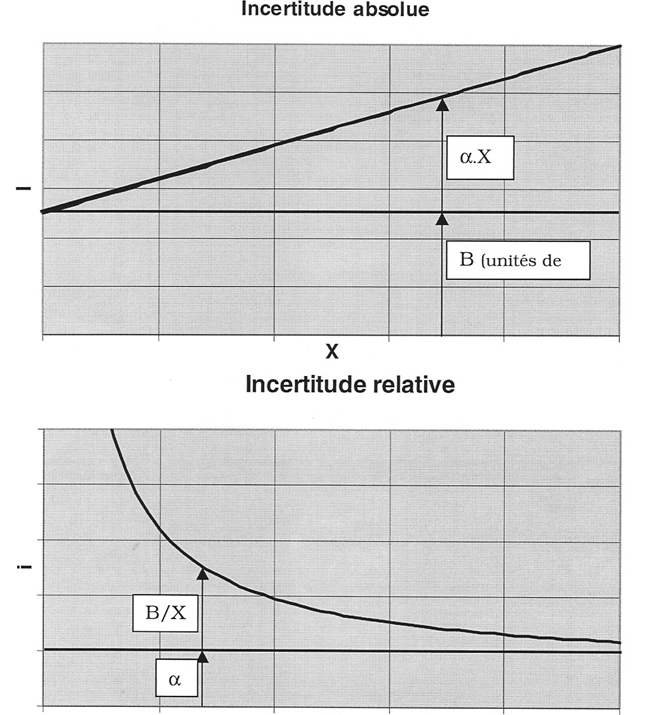
\includegraphics[height=10.7cm]{assets/figures/3_2_incertitudes_absolues_et_relatives.PNG}
\caption{Evolution des incertitudes absolues et relatives en fonction du mesurande.}
\label{fig:incertitudes_absolues_et_relatives}
\end{figure}

La figure~\ref{fig:incertitudes_absolues_et_relatives} nous montre que l'incertitude absolue est maximum en haut de gamme, alors que l'incertitude relative tend vers l'infini lorsque X tend vers zéro. Lorsqu'on doit évaluer l'imprécision d'un système de mesure, on le fera soit en estimant l'incertitude absolue en haut de gamme, soit l'incertitude relative en bas de gamme (recherche du pire des cas).

Lorsqu'on fait l'évaluation d'un mesurande qui évolue dans une plage de variation donnée, on cherchera avantageusement à relativiser l'incertitude par rapport à la pleine échelle (PE, en anglais FS pour "Full Scale") de cette variation, et de l'exprimer alors en \%(PE) ou \%(FS). Par exemple, l'information fournie par un capteur de pression qui évolue entre 950 et 1100 mbar permet bien de savoir à quel endroit se trouve la pression le long des 150mbar d'évolution possible. Dans ce cas c'est donc bien la pleine échelle qui nous intéressera comme référence.

Par ailleurs, lorsqu'on cherche à faire une mesure d'une grandeur avec un appareil donné, on remarquera souvent que la valeur B augmente quasi-proportionnellement avec la gamme alors que $\alpha$ reste assez stable quelle que soit la gamme. Ainsi, pour de bonnes mesures il est indispensable de choisir la plus petite gamme de mesure possible. On aura ainsi un B minimal.

\section{Calibrage et étalonnage}

Sur de nombreuses chaînes de mesure on dispose d'un amplificateur avec lequel on peut ajuster le gain et le décalage. On est alors amené, au moment de la mise en service de la chaîne, à ajuster cet amplificateur, de manière à obtenir la réponse la plus proche que possible de l'idéal (modèle nominal). C'est ce qu'on appelle le calibrage (en anglais: gauging ou calibration), opération qui vise à annuler les erreurs de gain et de décalage. Une autre opération consiste, sans modifier la chaîne, à déterminer son modèle réel, et l'écart entre le modèle réel et le modèle nominal. C'est l'opération d'étalonnage(en anglais: calibration). Cette opération peut être faite dans un but de correction ou de vérification. Dans ce dernier cas, la chaîne est acceptée si elle se trouve dans les tolérances, ou rejetée sinon. Dans le cas de la correction, alors un moteur de correction sera mis en oeuvre par l'utilisateur de la chaîne de mesure pour exploiter non pas le modèle nominal mais le modèle réel mesuré.
On notera que la terminologie française est cette fois plus précise que la terminologie anglaise où la distinction entre calibrage et étalonnage ne se fait pas. Ce flou se retrouve en français lorsqu'on utilise l'anglicisme "calibration", alors que ce terme s'applique normalement à des méthodes de datation en dendrochronologie.
\begin{center}
\fbox{
\begin{minipage}{0.96\textwidth}
\textbf{\textit{Déf}. Etalonnage :	}
Ensemble des opérations permettant de déterminer le modèle réel de la chaîne de mesure, et donc de déterminer les erreurs de mesure par rapport au modèle nominal.\\

\textbf{\textit{Déf}. Calibrage :	}
Ensemble des opérations d'ajustage des différents réglages de la chaîne, pour l'amener à un fonctionnement aussi juste que possible, c'est-à-dire aussi proche que possible du modèle nominal.
\end{minipage}
}
\end{center}

Dans ces opérations, il faut imposer à l'entrée de la chaîne une valeur connue du mesurande, et observer la sortie de la chaîne. Quatre situations peuvent se présenter :
\begin{enumerate}[a)]
\item Dans de très rares cas, on dispose d'un moyen d'imposer une valeur exacte (par exemple une tension nulle au moyen d'un court-circuit).
\item Parfois on dispose d'un étalon (par exemple 0 \degree C au moyen d'un mélange d'eau et de glace fondante), et la valeur imposée n'est connue qu'avec une certaine incertitude.
\item Dans la majorité des cas, il faut mesurer la grandeur d'entrée avec des instruments de précision, et  régler la valeur désirée, ce qui conduit également à une incertitude sur cette valeur.
\item Enfin il peut être impossible d'imposer une grandeur d'entrée connue et stable (par exemple 1200 \degree C), on procède alors par simulation du capteur en générant la grandeur électrique qu'il est censé produire (résistance, charge électrique, tension, etc.) sous l'effet de la grandeur physique désirée; l'incertitude provient alors d'une part de la qualité des générateurs, d'autre part de celle du capteur (on simule un capteur parfait, alors que le capteur réel ne l'est pas).
\end{enumerate}
L'idéal recherché généralement est de connaître le mesurande avec une incertitude inférieure à $1/10$ de l'incertitude de la chaîne à étalonner ou à calibrer.

\subsection{Calibrage}

Pour ajuster le gain et le décalage, il suffit de faire passer la réponse par deux points connus. Si ces 2 points sont choisis arbitrairement, il est évident que les deux réglages seront dépendants l'un de l'autre, et qu'il faudra procéder par approximations successives: imposer $X_{0}$, ajuster le décalage de la chaîne pour $Y_{0} = G_{nom} \cdot X_{0} + Of_{nom}$; puis imposer $X_{max}$ et ajuster le gain pour $Y_{max} = G_{nom} \cdot X_{max} + Of_{nom}$; revenir à $X_{0}$ et corriger le décalage ...etc.

Si l'on connaît la construction et les signaux à l'intérieur de la chaîne, alors on peut choisir $X_{0}$ de telle manière que le signal interne soit nul. Dans ce cas le gain n'influence pas l'ajustage du décalage, et l'opération peut se faire en deux étapes seulement.

L'ajustage des potentiomètres ne sera jamais exact : les bruits internes dans la chaîne et  la résolution du potentiomètre conduisent à une erreur d'affichage résiduelle.

Ainsi on applique généralement le mesurande X et on effectue plusieurs mesures Y qui permettent de déterminer une moyenne de la valeur appliquée et une moyenne de la valeur mesurée, ainsi que les minima et maxima. On détermine ainsi un rectangle d'incertitude. On établit ensuite un rectangle d'incertitude centré sur la valeur moyenne en maximisant les écarts autour de la valeur moyenne. Les valeurs moyennes permettront de déterminer le modèle réel.

\begin{figure}
\centering
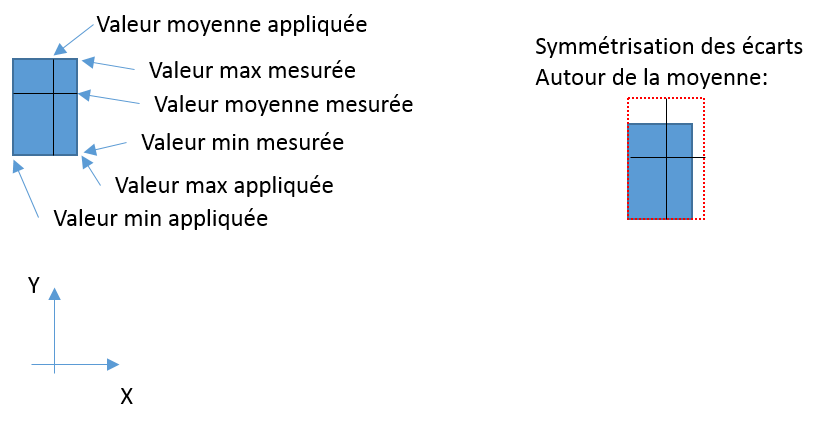
\includegraphics[width=12cm]{assets/figures/3_3_explications.PNG}
\caption{Un point de mesure, avec les incertitudes sur la valeur appliquée X et sur la valeur mesurée Y.}
\label{fig:3_3_explications}
\end{figure}

\begin{figure}
\centering
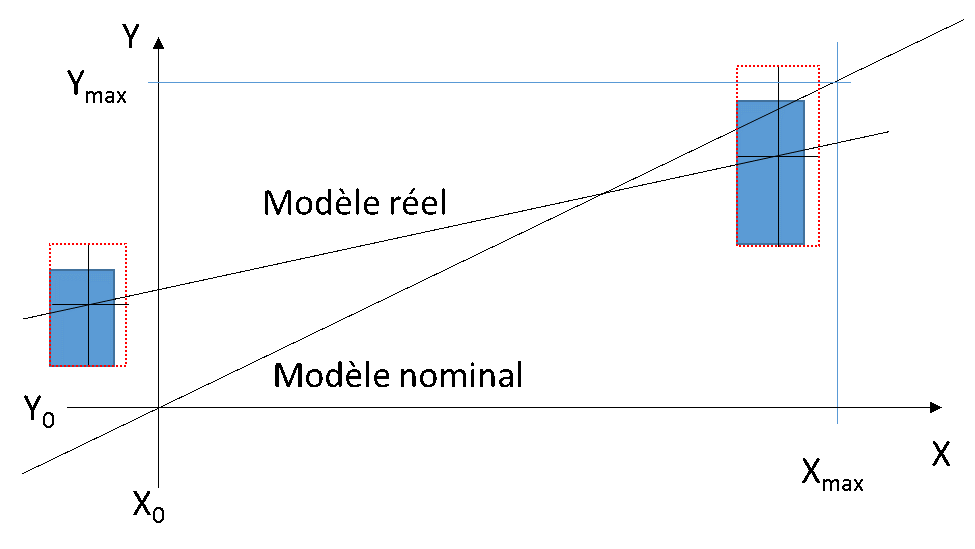
\includegraphics[width=12cm]{assets/figures/3_3a_reel_versus_nominal.PNG}
\caption{Mesure après calibrage: modèles nominal et réel.}
\label{fig:3_3a_reel_versus_nominal}
\end{figure}

\begin{figure}
\centering
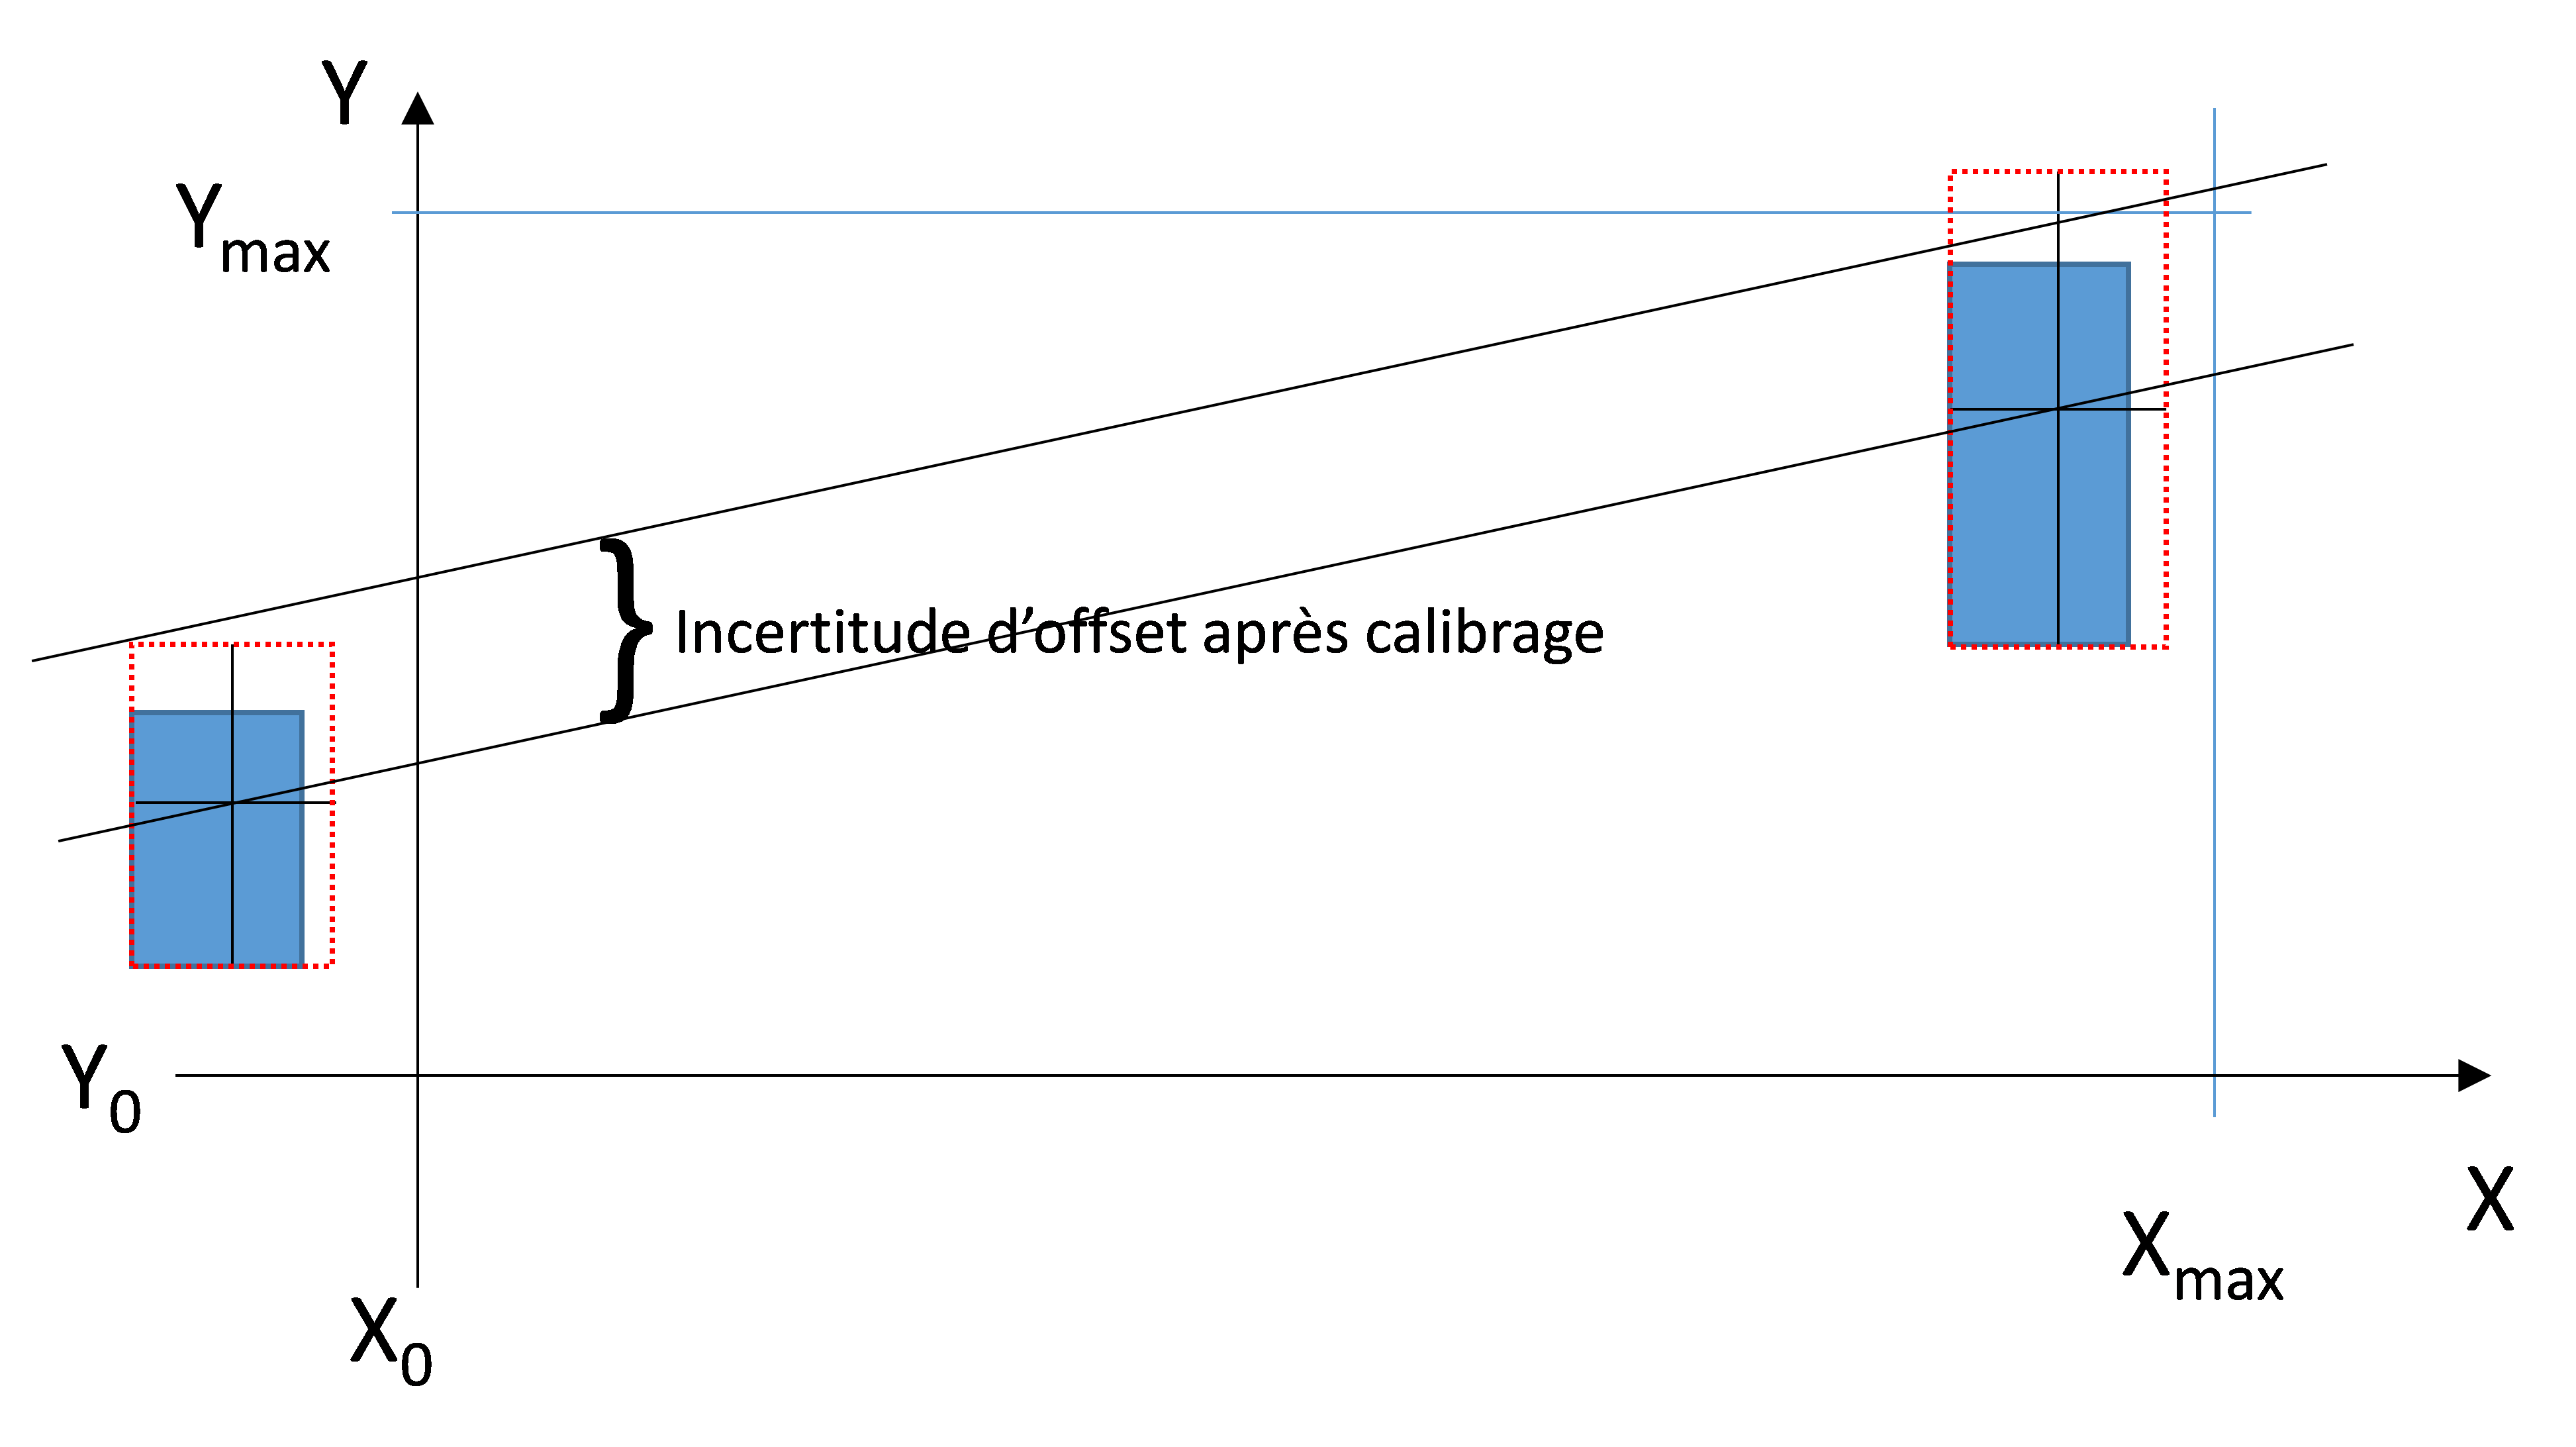
\includegraphics[width=12cm]{assets/figures/3_3b_incertitude_de_offset.PNG}
\caption{Mesure après calibrage: incertitude sur l'offset.}
\label{fig:3_3b_incertitude_de_offset}
\end{figure}

\begin{figure}
\centering
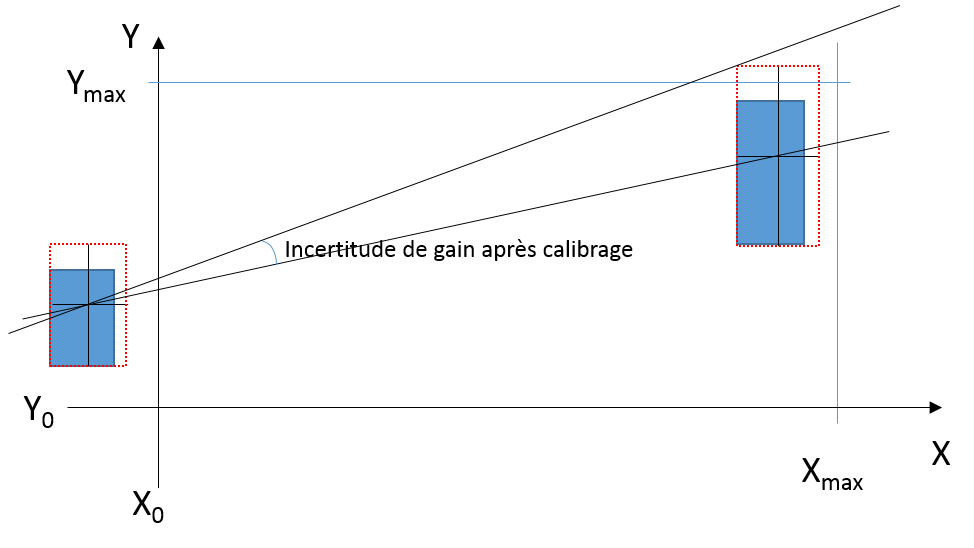
\includegraphics[width=12cm]{assets/figures/3_3c_incertitude_de_gain.PNG}
\caption{Mesure après calibrage: incertitude sur le gain.}
\label{fig:3_3b_incertitude_de_gain}
\end{figure}

En résumé, le calibrage consiste à :

\begin{center}
\fbox{
\begin{minipage}{0.96\textwidth}
\textbf{ }
\begin{itemize}
\item Imposer un mesurande $X_0$ nul correspondant au zéro de mesure, et ajuster le décalage de la chaîne pour obtenir l'offset du modèle nominal ; le zéro est le point sur lequel le gain n'a pas d'effet.
\item Imposer la valeur maximum $X_{max}$ de mesure et ajuster le gain (span) de la chaîne pour obtenir la valeur correpondante selon le modèle nominal.
\item Déterminer les incertitudes sur les valeurs ajustées et en déduire les incertitudes de calibrage:	$D_{c} = \Delta X_{o} + \frac{\Delta Y_{o}}{G} $ et
$\alpha _{c} = \frac{D_{c} + \Delta X_{max} + \frac{\Delta Y_{max}}{G}}{X_{max} -X_{o}} $
\end{itemize}
\end{minipage}
}
\end{center}

Après une opération de calibrage, on peut généralement considérer que les erreurs de gain et de décalage ont été annulées. Par conséquent, pour les mêmes valeurs des grandeurs d'influence (raisonnablement quelques minutes à quelques heures après le calibrage) seules interviennent les erreurs de non-linéarité et le bruit interne. C'est pourquoi, un calibrage préalable est très souvent utilisé dans les procédures de mesure. Dans ce cas on utilisera comme référence le modèle nominal.

Dans certains cas, lorsque les moyens de réglage ne nous permettent pas de nous rapprocher suffisamment du modèle nominal ou lorsqu'on cherche à améliorer la précision, alors on choisira comme référence le modèle réel obtenu par étalonnage, mesuré après calibrage. Dans ce dernier cas, alors les valeurs $\Delta X_{o}$ et $\Delta Y_{o}$ ainsi que $\Delta X_{max}$ et $\Delta Y_{max}$ seront généralement établies autour des valeurs moyennes de $\Delta X$ et $\Delta Y$.

Lorsqu'il n'est pas possible ou pas souhaitable d'appliquer un mesurande nul, l'évaluation des incertitudes suivra le même principe que ci-dessus, mais il faudra tenir compte du fait que chacun des points $X_{min}$ et $X_{max}$ influencent la réponse à $X_{0}$, et donc la valeur du décalage. Les relations pour $D_{c}$ et $\alpha_{c}$ ne sont alors pas valables.

\subsection{Etalonnage}

Ici, il faut établir un tableau de mesure, couvrant toute l'étendue de mesure. Manuellement on se contente d'une dizaine de mesures répartie entre le minimum et le maximum. Lorsqu'on utilise un système d'acquisition, on recherche un beaucoup plus grand nombre de mesures, couvrant plusieurs cycles sur l'étendue de mesure, de manière à permettre la mise en évidence de phénomènes éventuels tels que l'hystérèse, la répétabilité ou le bruit de mesure.

Pour chaque couple mesuré $(X(i), Y(i))$, on peut déterminer l'erreur
\[
e(i) = X_m(i) - X(i) = \frac{Y(i) - Of_{nom}}{G_{nom}}   -X(i)
\]
mais ceci ne nous permet pas de bien séparer les composantes de l'erreur.

Il convient donc de déterminer le modèle actuel de la chaîne, c'est-à-dire $G_{réel}$ et $Of_{réel}$, après quoi on pourra séparer les composantes d'erreur (gain, décalage, non-linéarité et bruit). La manière de définir la droite de réponse influence quelque peu les résultats, si bien qu'il est indispensable d'utiliser une définition commune, si l'on veut comparer les résultats (par exemple avec les spécifications individuelles des composants de la chaîne). On utilise généralement deux méthodes de choix de cette droite:
\begin{center}
\fbox{
\begin{minipage}{0.96\textwidth}
\textbf{Droite par les extrêmes (End points linearity) :}
la droite passe par deux points de la courbe de réponse réelle (en général le zéro et la pleine échelle, ou encore les deux extrémités du domaine de mesure).\\

\textbf{Meilleure droite (Best fit linearity) :}
C'est la droite de régression linéaire, elle minimise la somme des carrés des écarts entre la courbe de réponse réelle et la droite ainsi définie.
\end{minipage}
}
\end{center}

Le gain réel $G_{reel}$ est la pente de la droite ainsi choisie. Le décalage réel $D_{reel}$ est l'ordonnée à l'origine de la droite. Pour chaque couple mesuré $(X(i),Y(i))$ on détermine l'écart entre la valeur mesurée et la droite $\Delta = Y(i) - [G_{reel}\cdot X(i) + Of_{reel}]$. Cet écart est une combinaison de l'erreur de non-linéarité et du bruit. Pour une utilisation immédiate après le calibrage, cet écart représente l'erreur résiduelle du montage, et on en spécifie la limite maximum en valeur absolue, dans l'unité du mesurande, ce qui revient à diviser $max{|\Delta|}$ par le gain de la chaîne~:
\[
	NL+Bruit = \frac{max{|\Delta|}}{G_{reel}}
\]
Une séparation du bruit et de la non-linéarité n'est généralement pas nécessaire.
Les erreurs de gain et de décalage du modèle réel par rapport au modèle nominal se calculent en comparant $G_{reel}$ et $Of_{reel}$ avec $G_nom$ et $Of_nom$ :

\[\alpha =  \frac{G_{reel}-G_{nom}}{G_{nom}}	 \]
\[D =  \frac{Of_{reel}-Of_{nom}}{G_{nom}} \]

Dans certains cas on sera amené à établir les incertitudes de gain et de décalage du modèle réel par rapport à lui-même, dues à des instabilités constatées sur l'affichage et à des difficultés d'appliquer un mesurande parfaitement stable. Dans ce cas on procédera comme au point précédent pour l'établissement des incertitudes de calibrage.

\subsection{Auto-calibrage }
Les avantages apportés par un calibrage juste avant une série de mesures sont tels qu'il devient indispensable de le réaliser pour compenser les effets des grandeurs d'influence si l'on veut atteindre une haute précision. C'est pourquoi de nombreux équipements de précision incorporent une séquence automatique de calibrage (ou au moins d'ajustage du zéro = auto-zéro) à intervalles réguliers ou même avant chaque mesure. Ce calibrage peut se faire de manière analogique ou entièrement numérique.
Pour permettre un auto-calibrage, il suffit d'insérer un commutateur permettant de déconnecter l'entrée normale de mesure pour la remplacer par les étalons correspondant à $X_0$ et à $X_{max}$. La séquence de travail lors du calibrage est semblable à la séquence manuelle, si ce n'est qu'il faut mémoriser les valeurs de correction. Ensuite, il faut soit agir sur les réglages matériels, soit utiliser un moteur de correction, qui n'est en fait rien d'autre qu'un calculateur. Si ce calculateur se trouve dans la chaîne de mesure et que celle-ci fournit une sortie numérique ainsi calibrée, alors on a bien un auto-calibrage. Toutefois dans certains cas la chaîne de mesure fournit d'une part le signal sans correction, d'autre part les paramètres de correction. Dans ce dernier cas, on parlera alors d'auto-étalonnage.

\section{Compensation des erreurs systématiques}

Au lieu d'un auto-calibrage, il est parfois plus efficace de faire une compensation directe d'une erreur systématique, s'il est possible d'identifier son influence. Un cas typique se présente dans les capteurs de pression intégrés où la température est l'influence prépondérante ; souvent c'est également l'influence de la tension d'alimentation qu'il faut pouvoir compenser.

\subsection{Compensation linéaire }
L'identification consiste à déterminer les coefficients d'influence agissant sur le gain et le décalage de la chaîne. Généralement on se contente de déterminer $G_r$ et $Of_r$ aux deux valeurs extrêmes d'utilisation. En faisant l'hypothèse que l'évolution du gain et celle du décalage sont linéairement dépendantes de la grandeur d'influence, on définit les coefficients d'influence :

\begin{center}
\fbox{
\begin{minipage}{0.96\textwidth}
\textbf{\textit{Déf}. Coefficient d'influence sur le gain : }
variation relative du gain par unité de la grandeur d'influence. Représente l'erreur de gain additionnelle due à la grandeur d'influence $Z_i : d\alpha / dZ_i = (dG_r/G_r)/dZ_i$ (proportionnelle à X : exprimée en$ \%/unité de Z_i$)
\\
\\
\textbf{\textit{Déf}. Coefficient d'influence sur le décalage :}
variation d'offset par unité de la grandeur d'influence. Représente l'erreur de décalage additionnelle due à la grandeur d'influence $Z_i$ : \\
\begin{equation}
{dD}{dZ_i} = \frac{(dOf_r/G_r)}{dZ_i}\text{ }[\frac{unites de X}{unites de Z_i}]
\end{equation}
\end{minipage}
}
\end{center}

Pour effectuer la correction, il suffit alors de mesurer $Z_i$ (chaîne auxiliaire), d'en déduire la variation par rapport à la valeur de $Z_i$ au moment du calibrage, et de multiplier les coefficients d'influence par cet écart pour connaître la variation de gain ou de décalage par rapport au calibrage.

A titre d'exemple prenons un capteur de pression intégré. La grandeur d'influence est la température T. On commence par étalonner le capteur aux deux températures extrêmes d'utilisation, ici environ 25 et 60 \degre C. Une telle mesure est présentée sur le graphique ci-dessous.

\begin{figure}
\centering
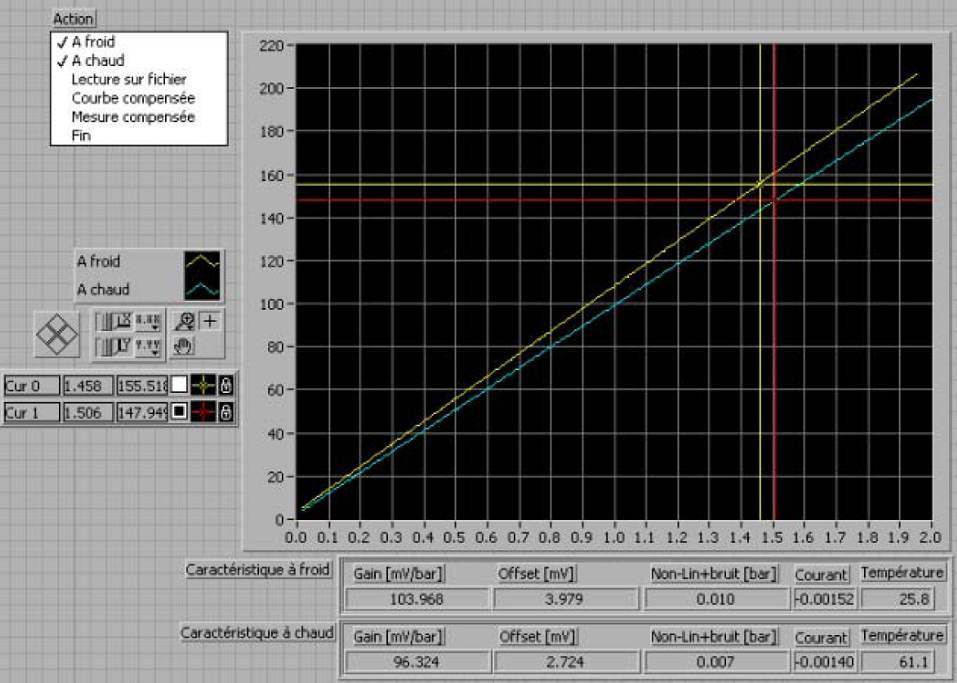
\includegraphics[height=10cm]{assets/figures/3_5_identification_reponse_en_temperature.PNG}
\caption{ Identification de la réponse du capteur aux températures extrêmes.}
\label{fig:IdentificationTemperature}
\end{figure}

On en déduit les coefficients d'influence, en prenant les valeurs exactes mesurées à une température de calibrage, ici 25.8 \degre C :
Gain:
\[
\frac{d\alpha}{dT} = \frac{dGr/Gr}{dT} = \frac{(96.324-103.968)/103.968}{ (61.1-25.8)} =\]
\begin{equation}
= \frac{-0.0735}{35.3} = -0.002083 = -0.21 \% \text{/ \degre C}
\end{equation}

Décalage:
\begin{equation}
\frac{dD}{dT} = \frac{(dOfr/Gr)}{dT} = \frac{(2.724-3.979)/103.968}{(61.1-25.8)} =
 \frac{-0.012 bar}{ 35.3 \text{\degre C}} = -0.34 \text{mbar/ \degre C}
\end{equation}

Par conséquent, si l'on mesure alors que la température est de 38.0 \degre C, nous avons un écart de température de (38.0 - 25.8) = 12.2 \degre C et les erreurs additionnelles de gain et de décalage par rapport aux valeurs de calibrage (gain 103.968 mV/bar et offset 3.979 mV) seront de :

$d\alpha = -0.002083 \cdot 12.2 = -0.0254 = -2.54 \% lect $
\\
$dD = -0.34 m \cdot 12.2 = - 4.148 mbar $

Pour corriger les indications il est généralement plus simple de calculer le gain et l'offset actuels avant de traduire la sortie (mV) en valeurs de pression :

$G(38 \text{\degre C}) = G(25.8 \text{\degre C}) (1 + d \alpha) = 103.968(1-0.0254) = 101.327 mV/bar $
\\
\\
$Of(38 \text{\degre C}) = Of(25.8 \text{\degre C}) + G(25.8 \text{\degre C}) \cdot dD = 3.979 - 4.148 \cdot 10-3 \cdot 103.968 = 3.548 mV$
\\

Ainsi une sortie de 89 mV correspond à une pression de (89-3.548) / 101.327 = 0.843 bar.

Sans correction, avec les valeurs de calibrage on obtient 0.731 bar : on sous-évalue la pression car la température introduit un décalage négatif de -4.2 mbar ainsi qu'une erreur de gain négative de -2.54\% de 731 mbar soit -15.6 mbar, et donc un total de -19.8 mbar.

\subsection{Moteur de correction mathématiques}

La puissance de calcul des microprocesseurs incorporés aux capteurs dits \textless\textless\ intelligents \ \textgreater\textgreater permet d'envisager des corrections bien plus efficaces, qui sont maintenant incorporées dans les profils d'utilisation de ces capteurs (réseau de terrain).
A titre d'exemple, la norme IEEE-1451 / Smart Transducers, définit une fonction multi - variables, de type polynomial, et décomposable par segments :

\begin{equation}
\displaystyle\sum_{i=0}^{D(1)}
\displaystyle\sum_{j=0}^{D(2)} \text{...}
\displaystyle\sum_{p=0}^{D(n)} C_{i,j,...,p} [X_1-H_1]^i[X_2-H_2]^j \text{...} [X_n-H_n]^p
\end{equation}

Le calcul de correction ci-dessus représente une somme polynomiale de n variables, dont on peut choisir indépendamment les degrés de chaque variable. Dans le cas de la compensation linéaire de température, nous aurions $X_1$ = sortie en mV du capteur de pression, $X_2$ = sortie du capteur de température, les degrés D(1) et D(2) seraient tous deux égaux à 1 (linéaire), et la formule permet de calculer la valeur de pression. Par conséquent la formule de calcul devient :
\begin{equation}
P_m =C_{00} + C_{10} \cdot (X_1-H_1)+C_{01} \cdot (X_2-H_2) + C_{11}\cdot(X_1-H_1) \cdot (X_2-H_2)
\end{equation}

\begin{equation*}
= C_{00} + C_{01} \cdot X_2 + X_1 \cdot (C_{10} + C_{11} \cdot X_2)  \text{ si les termes $H_1$ et $H_2$ sont nuls }
\end{equation*}

On voit bien qu'ainsi on a bien un décalage $(C_{00} + C_{01} \cdot X_2)$ dépendant de $X_2=T$ et un gain $(C_{10} + C_{11} \cdot X_2)$ également dépendant de T. Par contre cette méthode permet des corrections bien plus évoluées (polynômes et compensation de plusieurs grandeurs d'influence).

Pour de grands domaines ou pour de fortes non-linéarités, afin d'éviter des polynômes de degré trop élevé, la norme prévoit de segmenter la réponse selon les valeurs des différentes variables, et d'exploiter un ensemble de paramètres de faible degré dans chaque segment, comme illustré dans la figure ci-dessous.

\begin{figure}
\centering
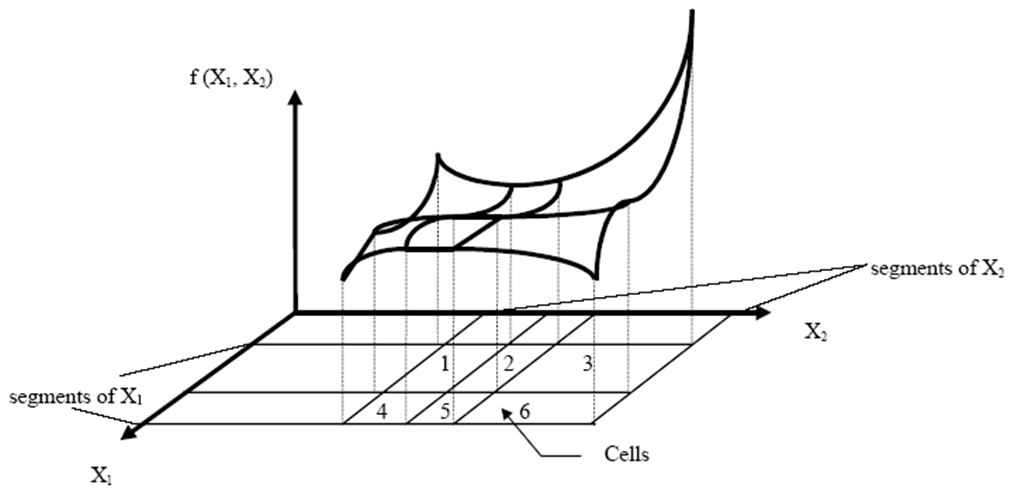
\includegraphics[height=6cm]{assets/figures/3_6_Correction_a_2_variables_segementees.PNG}
\caption{Correction à deux variables segmentées.}
\label{fig:Correction_a_2_variables_segementees}
\end{figure}

A chaque élément de surface (désigné par "Cell") correspond un ensemble de paramètre $C_{ij}$ et $H_x$ permettant d'approcher la surface réelle en minimisant le nombre total de paramètres à mémoriser.

\section{Mesures répétées}

Lors de mesures répétées de la même valeur du mesurande X, on constate que les résultats ne sont pas toujours parfaitement ceux qu'on attend, et ne sont pas identiques. Une analyse statistique des résultats de mesure permettra d'établir une valeur moyenne $\mu$ de tous les résultats ainsi qu'un écart-type $\sigma$. Les mesures sont en général réparties autour de la moyenne selon une distribution gaussienne caractérisée par cet écart-type. Ainsi la moyenne constitue la partie systématique de l'erreur appelée aussi le biais, alors que l'écart-type représente sa composante aléatoire.

\newpage
On a donc :
\begin{itemize}\itemsep1pt
\renewcommand{\labelitemi}{$\bullet$}
\item X, le mesurande
\item La moyenne des mesures $\mu$
\item L'erreur de biais $\beta :  \beta = \mu - X$  [unité de X], erreur systématique
\item L'exactitude ou la justesse, termes utilisés pour caractériser l'erreur systématique
\item L'écart-type $\sigma$ sert à quantifier l'erreur aléatoire
\item La répétabilité ou la fidélité, termes utilisés pour caractériser l'erreur aléatoire
\end{itemize}

\begin{equation}
\mu = \lim\limits_{N \to \infty} \frac{1}{N} \sum_{i=1}^N x_i
\end{equation}

\begin{equation}
\sigma = \lim\limits_{N \to \infty} \sqrt{\frac{1}{N}\sum_{i=1}^N (x_i-\mu)^2}
\end{equation}

\begin{figure}
\centering
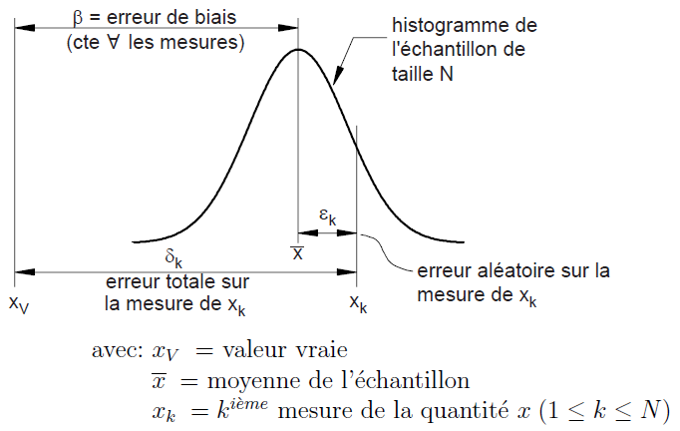
\includegraphics[height=7cm]{assets/figures/3_7_Exemple_de_mesures_repetees_N_fois.PNG}
\caption{Exemple de mesures répétées N fois, où N >100 pour être significatif.}
\label{fig:Exemple_de_mesures_repetees_N_fois}
\end{figure}

\begin{figure}
\centering
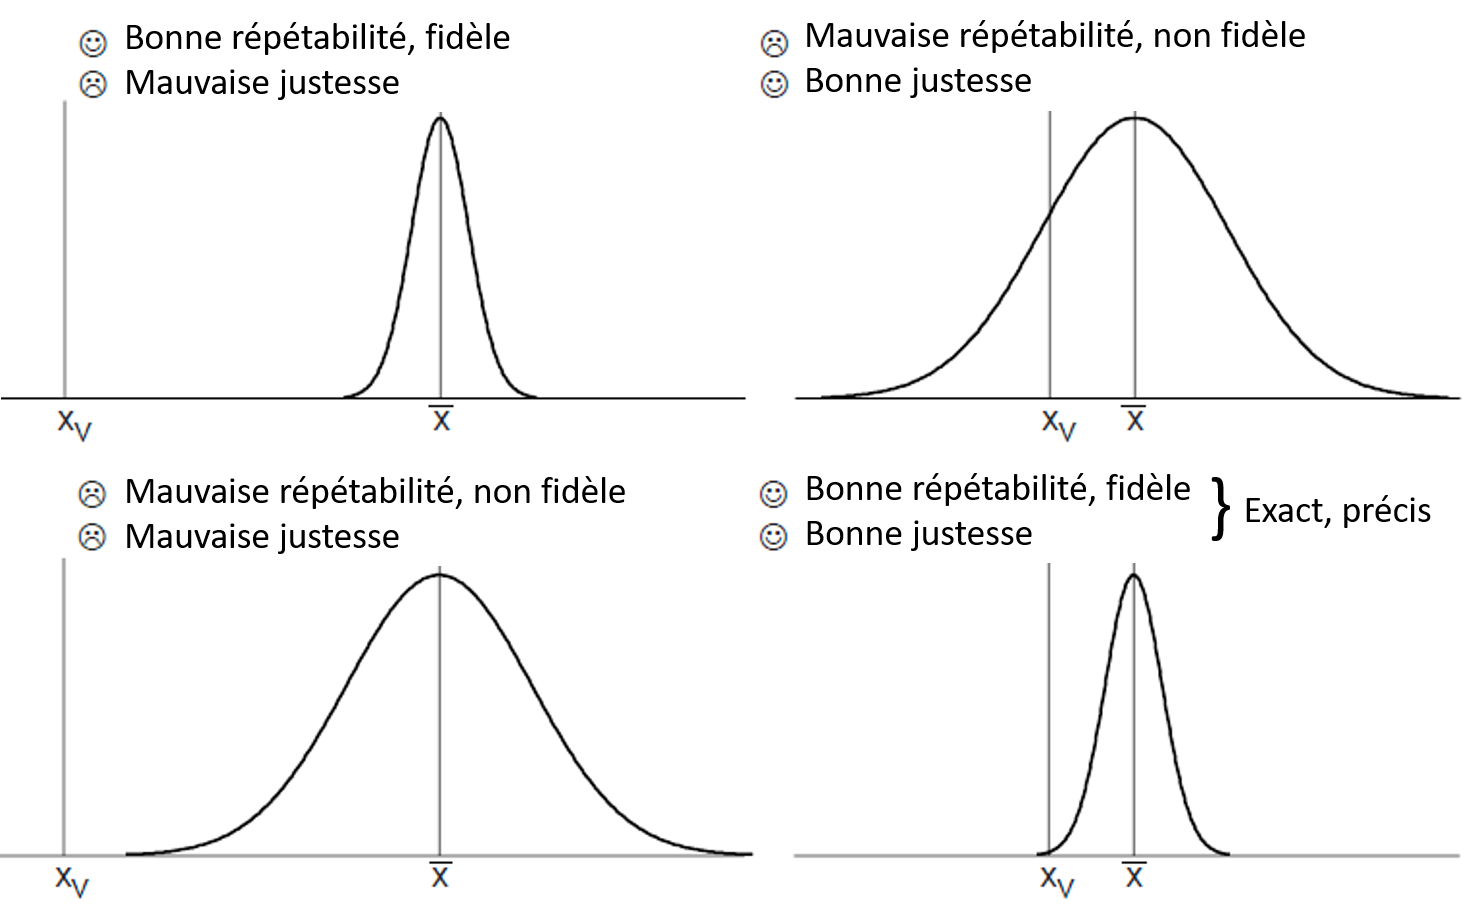
\includegraphics[height=7cm]{assets/figures/3_8_distinction_entre_repetabiite_et_justesse.PNG}
\caption{distinction entre répétabilité et justesse.}
\label{fig:distinction_entre_repetabiite_et_justesse}
\end{figure}

\begin{figure}
\centering
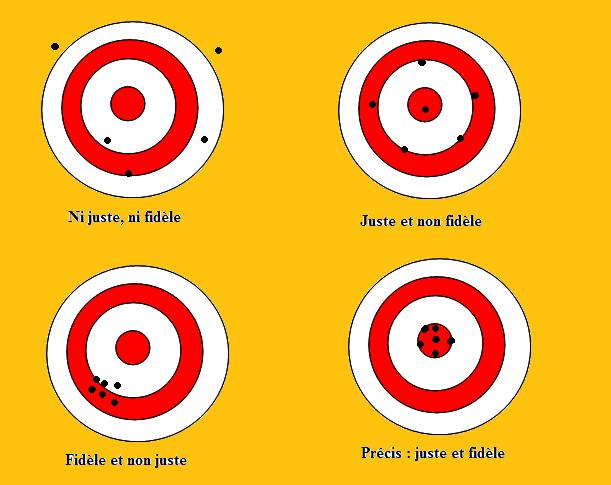
\includegraphics[height=7cm]{assets/figures/3_8b_juste_fidele_precis.PNG}
\caption{Autre représentation des notions de justesse et fidélité.}
\label{fig:juste_fidele_precis}
\end{figure}

L'écart-type sert à mesurer la dispersion d'un ensemble de données. Plus il est faible, plus les valeurs sont regroupées autour de la moyenne. Par exemple pour la répartition des notes d'une classe, plus l'écart type est faible, plus la classe est homogène. ¿ l'inverse, s'il est plus important, les notes sont moins resserrées. Dans le cas d'une notation de 0 à 20, l'écart-type minimal est 0 (notes toutes identiques), et peut valoir jusqu'à 10 si la moitié de la classe a 0/20 et l'autre moitié 20/20.

En sciences, il est fréquent de considérer que les valeurs se répartissent selon une courbe de Gauss. Dans le cas des sciences sociales, par exemple, la moyenne $\mu$ et l'écart-type $\sigma$ permettent de déterminer un intervalle dans lequel on trouve une majorité de la population. En effet, si la moyenne est $\mu$ et l'écart type est $\sigma$, on trouve 95 \% de la population dans l'intervalle $[ \mu - 1.96 \sigma ; \mu + 1.96 \sigma ]$ et on trouve 68.2 \% de la population dans l'intervalle $[ \mu - \sigma ; \mu + \sigma ]$.

L'écart-type est aussi utilisé pour construire un intervalle de confiance attribuable à un échantillon. Si l'on se réfère à la figure ci-contre, on voit qu'un $\sigma$ d'écart de part et d'autre de la valeur moyenne recouvre 68,2\% de la distribution, deux $\sigma$ d'écart $(13.6+34.1+34.1+13.6 =) 95.4\%$, 3 $\sigma$ d'écart $(2.1+13.6+34.1+34.1+13.6+2.1 =) 99.6\%$ et ainsi de suite... C'est l'usage notamment en physique des particules, où la détection d'évènements est quantifiée en nombre de sigmas, et où un résultat notamment est considéré comme significatif par l'obtention de 5 $\sigma$, représentant une probabilité d'erreur inférieure à 0,00003\% (niveau de confiance de plus de 99.99997\%).

En pratique, on considère que :
\begin{itemize}\itemsep1pt
\renewcommand{\labelitemi}{$\bullet$}

\item $1 * \sigma \rightarrow 68\% $
\item $2 * \sigma \rightarrow 95\% $
\item $3 * \sigma \rightarrow 99.7\%$

\end{itemize}


\begin{figure}
\centering
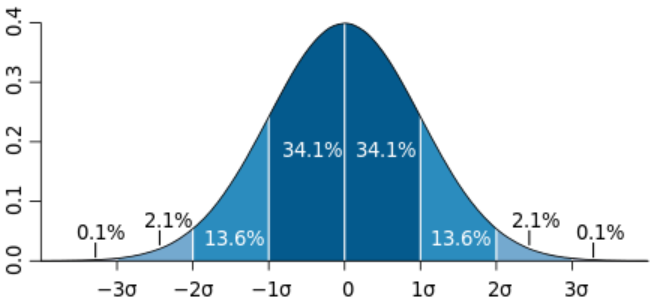
\includegraphics[height=7cm]{assets/figures/3_9_Loi_normale_et_intervale_de_confiance.PNG}
\caption{Loi normale et intervale de confiance.}
\label{fig:3_9_Loi_normale_et_intervale_de_confiance}
\end{figure}

\section{Exercices }

\subsection{Exercice: Incertitudes des appareils }
Spécifications:\\
\\
\textbf{HP34401A}: spécifs pour 1 an, $23 \pm 5 \degree C$, en (\%lect+ \%gamme) et jusqu'à 20\% de dépassement de gamme\\
\\
\begin{tabular}{l c c}
\hline
gamme: 	& 100.0000 mV	& 0.0050 + 0.0035 \\
		& 1.000000 V	& 0.0040 + 0.0007 \\
    	& 10.00000 V	& 0.0035 + 0.0005 \\
		& 100.0000 V	& 0.0045 + 0.0006 \\
		& 1000.000 V	& 0.0045 + 0.0010 \\
\hline
\end{tabular}
\\
\\
\textbf{Prema} 6000:spécifs pour 1 an, $23 \pm 5 \degree C$, en (\% of reading + \% of full scale)
	Full scale : 1'999'999 (sauf gamme 1000 V : 1'000'000)
\\
\begin{tabular}{lcc}
\hline
range & $\pm$ 0.2 V & 0.006 + 0.0007 \\
	& $\pm$ 2 V	& 0.005 + 0.0005 \\
	& $\pm$ 20 V	& 0.005 + 0.0006 \\
	& $\pm$ 200 V	& 0.005 + 0.0006 \\
	& $\pm$ 1000 V	& 0.006 + 0.0005 \\
\hline
\end{tabular}
\\
\\
\textbf{APPA-98}: spécifs pour 2 ans, $23 \pm 5 \degree C$ et moins de 75\% humidité relative, en (\% reading + number of digits)
\\
\begin{tabular}{lcl}
\hline
	Range	& Resolution	& Accuracy \\
	200 mV	& 100 $\mu$V	& | \\
	2 V	& 1 mV	& | \\
	20 V	& 10 mV	& |  $\pm$ (0.5 \%rdg + 1 dgt) \\
	200 V	& 100 mV	& | \\
	1000 V	& 1 V	& | \\
\hline
\end{tabular}
\\

\begin{enumerate}
\item Quelles sont les incertitudes absolues et relatives si on mesure 2.2 V avec HP34401A ?
\item Quelles sont les incertitudes absolues et relatives si on mesure 2.2 V avec APPA-98 ?
\item Quelle est l'incertitude relative maximum si on mesure entre 10 et 250 mV avec HP34401A ?
\item Quelle est l'incertitude relative maximum si on mesure entre 10 et 250 mV avec Prema6000 ?
\item Quelle est l'incertitude absolue maximum si l'on mesure entre 30 et 500 V avec APPA-98 ?
\item Représenter les incertitudes relatives du HP34401A et du Prema6000 pour un domaine de 10mV à 1000V (utilisez une échelle Log pour l'axe X des tensions).
\end{enumerate}
NB: la pleine échelle définie pour le PREMA n'est pas la définition habituelle qui dit que la pleine échelle est la différence entre les valeurs min et max. On aurait alors attendu pour le PREMA une pleine échelle égale au double de la gamme.

\subsection{Exercice: Calibrage d'une chaîne}
a)	Une chaîne de mesure de température doit être utilisée pour la régulation de température d'une enceinte, autour de 60 $\degree$ C. On désire qu'elle nous indique l'erreur (température actuelle moins consigne de 60 $\degree$ C). Le calibrage est réalisé ainsi: \\
i)	on place le capteur dans un bain à 60 $\pm$ 0.35 $\degree$ C, et on ajuste le décalage pour un affichage nominal de 0.00. On constate que les indications oscillent entre -0.03 et + 0.08. \\
ii)	on place le capteur dans un bain à 70 $\pm$ 0.5 $\degree$ C, et on ajuste le gain pour un affichage nominal de 10.00. On constate que les indications oscillent entre 9.88 et 10.09. \\  ~ \\
Quelles sont les incertitudes de gain et de décalage dues à ce calibrage ? \\

b)	Une chaîne de mesure doit indiquer l'épaisseur d'une feuille plastic (capteur capacitif sans contact, basé sur la variation de la constante diélectrique). Le calibrage s'effectue comme suit: \\
i)	Pas de feuille dans le capteur, on ajuste le décalage et on obtient un affichage stable de 000. \\
ii)	On place une feuille étalon d'épaisseur 0.500  $\pm$  0.005 mm dans le capteur, et on ajuste le gain pour un affichage nominal de 500. Malheureusement le potentiomètre ne permet pas l'ajustage exact et on doit se contenter d'un affichage oscillant entre 497 et 499. \\~ \\
Quelles sont les incertitudes de calibrage de cette chaîne ? \\

c)	Une chaîne de mesure de la hauteur du liquide contenu dans un réservoir utilise la pression relative à la base de ce réservoir (P = $\rho\,gh$ où h est la hauteur du liquide dans le réservoir). Pour le calibrage on procède comme suit: \\
i)	Réservoir vide, on ajuste le décalage pour un affichage de 0000  $\pm$  0001 \\
ii)	On remplit le réservoir, on mesure une hauteur h = 10.00 $\pm$ 0.02 m, ainsi que la densité du liquide  $\rho$ = 0.800  $\pm$  0.006 kg/dm3, et on ajuste l'affichage à 1000  $\pm$  0003 \\ ~ \\
Quelles sont les incertitudes de calibrage (indication: n'oubliez pas que la chaîne est sensible à la pression et non directement à la hauteur du liquide)? \\

d)	On a calibré un capteur de pression relative (=différence de pression par rapport à l'atmosphère) de la manière suivante : pression appliquée par une pompe dans la tuyauterie du capteur avec une vanne de détente, mesure de la pression appliquée par la différence de hauteur de mercure dans un tube en U, ouvert sur l'atmosphère, lecture de la sortie dans un PC. La réponse nominale est 0 à +2 bar, 0 à +20'000digit (1 bar = 100kPa). \\
i)	Vanne ouverte (= pression atmosphérique), ajustage de l'offset pour une valeur nominale de 0, on obtient un affichage stable de 00'000digit. \\
ii)	Vanne fermée, on agit sur la pompe jusqu'à une hauteur de mercure de 148.5 $\pm$ 0.2cm dans le tube en U. On calcule alors la pression appliquée $P=\rho\,gh = 13.6\times10^3 \text{ kg/m}^3 * 9.81\text {m/s}^2 * 1.485\text{ m}=198.12276\text{ kPa} = 1.98123\text{ bar}$. On ajuste donc le gain pour obtenir un affichage nominal de 19'812.3 digit, et obtient un affichage oscillant entre 19'810 et 19'814. \\ ~\\
Quelles sont les incertitudes de calibrage ?

\subsection{Exercice: Linéarité}

a)On a mesuré la réponse d'un capteur de force à $23 \degree C$ (réponse idéale : $0-100N \Leftrightarrow 0-20 mV$):\\
~
\\
\begin{tabular}{|l|l|l|l|l|l|l|l|l|l|l|l|}
\hline
F [N]	& 0	& 10	& 20	& 30	& 40	& 50	& 60	& 70	& 80	& 90	& 100 \\
\hline
U [mV]	& 0.50	& 2.49	& 4.46	& 6.41	& 8.34	& 10.25	& 12.14	& 14.01	& 15.86	& 17.69	& 19.5 \\
\hline
\end{tabular}
\\

Déterminez l'offset réel en [mV], le gain réel en [mV/N], les erreurs de décalage [N], de gain [\%lect] et l'incertitude de non-linéarité en [N] et en [\%(PE)] de ce montage par les deux méthodes :
\begin{enumerate}
\item Choix de la droite de référence par les extrémités de la courbe de réponse
\item Choix de la "meilleure droite"	 ...
\end{enumerate}
~\\

b)	L'étalonnage d'une chaîne de mesure de couple, gamme 0 à 100 mNm, sortie 4 à 20 mA, a donné: \\
~
\\
\begin{tabular}{|l|l|l|l|l|l|l|l|l|l|l|l|}
\hline
\footnotesize C [mNm]	& 0	& 10	& 20	& 30	& 40	& 50	& 60	& 70	& 80	& 90	& 100 \\
\hline

\footnotesize I [mA]	& \footnotesize  3.960	& \footnotesize  5.564	& \footnotesize  7.192	& \footnotesize  8.800	& \footnotesize  10.443	& \footnotesize  12.063	& \footnotesize  13.677	& \footnotesize  15.315	& \footnotesize  16.926	& \footnotesize  18.550	& \footnotesize  20.160 \\
\hline
\end{tabular}
\\

L'équation nominale de cette chaîne vaut donc $I = 4 [mA] + 0.16 [\frac{mA}{mNm}]  \cdot C [mNm]$.

Quelles sont les erreurs de gain et de décalage ainsi que l'incertitude de non-linéraité + bruit dans les 2 cas suivants:
\begin{enumerate}
\item Choix de la droite de référence par les extrémités de la courbe de réponse
\item Choix de la "meilleure droite"	 ...
\end{enumerate}

\subsection{Exercice: Auto-Calibrage d'une chaîne}

a)	Pour réaliser l'auto-calibrage d'un canal de mesure de courant (nominal 0-20 mA, code numériques 0-2000 digits), on procède comme suit:
\begin{itemize}\itemsep1pt
\renewcommand{\labelitemi}{$\bullet$}
\item ouverture du circuit de mesure par un interrupteur (donc courant nul), mémorisation du code obtenu :  $N_0=2$ (stable)
\item Fermeture d'un interrupteur reliant une source de tension de référence ($U_g = 10.000V \pm 0.005V$) au circuit de mesure à travers une résistance de $R_g = 500 \Omega \pm 0.1\%$ (la borne de mesure étant supposée travailler à potentiel nul, le courant nominal ainsi imposé est de 20mA). On mémorise alors le code moyen obtenu sur 10 mesures : $N_1 = 2018.3$, alors que les codes max et min sont 2021 et 2015.
\item Les mesures seront ensuite corrigées à l'aide de $N_0$ et $N_1$ pour obtenir :
	\begin{itemize}\itemsep1pt
	\renewcommand{\labelitemi}{$\bullet$}
	\item i) une valeur numérique corrigée ;
	\item ii) une valeur dans l'unité du mesurande ;
	\end{itemize}
\end{itemize}
NB : si ces corrections sont faites à l'extérieur de la chaîne de mesure, alors on parlera d'auto-étalonnage.
Quelles sont les fonctions mathématiques de correction et quelles sont les incertitudes de calibrage ?\\

b)	Pour programmer l'auto-calibrage d'une chaîne de mesure de température dont le capteur (PT100 : $R(T)=100 \Omega (1+0.00385T)$ a une interchangeabilité de 0.2 $\degree$ C + 0.1\%lecture, on a inséré des interrupteurs programmables permettant de déconnecter le capteur et de le remplacer soit par une résistance de$ 100 \Omega \pm 0.1 \Omega$, soit par une résistance de $138.5 \Omega \pm 0.14 \Omega$. La séquence d'auto-calibrage est la suivante :
\begin{itemize}\itemsep1pt
\renewcommand{\labelitemi}{$\bullet$}
\item Capteur remplacé par la résistance de $100 \Omega$, on mémorise la moyenne de 100 conversions: on trouve $M_0=1985.65$, toutes les conversions sont soit 1985, soit 1986.
\item Capteur remplacé par la résistance de $138.5 \Omega$. On mémorise la moyenne de 100 conversions: $M_1=2825.45$, conversion maximum 2827, minimum 2824.
\item Pour les mesures on ne fait qu'une seule conversion $N_x$, et l'on calcule \\
$T= (N_x - M_0)\frac{100}{M_1 - M_0}$
\end{itemize}
Quelles sont les incertitudes de calibrage ? \\

c)	Une chaîne de mesure de pression est constituée d'un capteur-transmetteur avec les spécifications suivantes : gamme -1 à +3 bar, sortie 4 à 20mA, précision 0.5\%lect + 35 mbar ; le courant de sortie est mesuré par une résistance shunt de $10 \Omega \pm 0.012 \Omega$, et un convertisseur gamme $\pm 0.25V$.
Pour programmer l'autocalibrage de cette chaîne, on a inséré des interrupteurs programmables permettant de déconnecter le capteur et de le remplacer soit en laissant le circuit ouvert, soit en reliant une résistance de $490 \Omega \pm 0.2 \Omega$ entre la borne positive du shunt et une source de tension de $+10V \pm 15mV$ (courant nominal de 20 mA). La séquence d'auto-calibrage est la suivante :
\begin{itemize}\itemsep1pt
\renewcommand{\labelitemi}{$\bullet$}
\item Capteur déconnecté, circuit ouvert on mémorise la moyenne de 100 conversions: on trouve $M_0=-0.73$ digit, toutes les conversions sont soit -1, soit 0 digit.
\item Capteur déconnecté, résistance $490 \Omega$ enclenchée. On mémorise la moyenne de 100 conversions: $M_1=1647.32$, conversion maximum 1646, minimum 1649 digit.
\item Les valeurs de $M_0$ et $M_1$ nous permettent de calculer le gain et l'offset total actuel de la chaîne.
\end{itemize}

Quelles sont les incertitudes de calibrage ?

\subsection{Exercice: Coefficients d'influence}

a)	On a étalonné une chaîne de mesure de position à deux températures:


\begin {center}
\begin{tabular}{lll}
$T_1=25 \degree C$ &	$G_1= 100.3 digit/mm$ &	$Of_1 = 3.4 digit$ \\
$T_2=75 \degree C$ &	$G_2 = 103.5 digit/mm$ &	$Of_2 = -5.8 digit$ \\
\end{tabular}
\end{center}
~\\
\begin{itemize}\itemsep1pt
\renewcommand{\labelitemi}{$\bullet$}
\item Déterminer les coefficients d'influence de la température
\item A une température de 40 $\degree$ C, l'indication obtenue est de 1380 digit. Calculer la position correspondante
\end{itemize}
~\\


b)	Une chaîne de mesure du contenu d'un réservoir utilise un capteur de force à jauges de contraintes (pont de Wheatstone à 4 jauges)

\begin{figure}[h!]
\centering
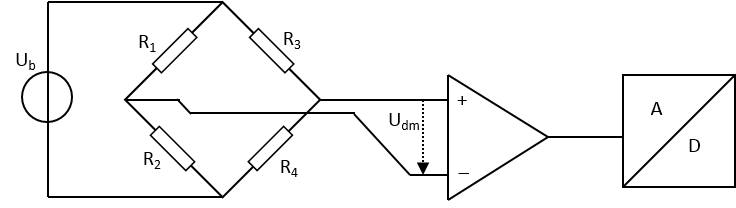
\includegraphics[height=3.7cm]{assets/figures/Exercice_3_5_c.PNG}
\caption{Chaîne de mesure du contenu d'un réservoir.}
\label{fig:Exercice_3_5_c}
\end{figure}

\begin{center}
$R_1 = R_4 = R_0(1 + F \cdot K)$\\
$R_2 = R_3 = R_0(1 - F \cdot K)$\\
\end{center}

Avec K = facteur de jauge et F = force appliquée.\\

On en déduit :	$U_{dm} = U_b ( \frac{ R_4}{R_3+R4} - \frac{R2}{R1+R2} ) = U_b \frac{ Ro(1+KF) -Ro(1-KF)}{2Ro}  = Ub \cdot K \cdot F$ \\
La sortie est donc théoriquement proportionnelle à la force, mais aussi à la tension d'alimentation $U_b$, on parle alors de capteur ratio-métrique : la sortie est une fraction (ratio) de l'alimentation.

On a étalonné la chaîne dans les 3 conditions suivantes :\\

\begin {center}
\begin{tabular}{llll}
$U_b = 5V$ &	$T=25 \degree C$ &	$G_1 = 1015 digit/tonne$ &	$Of_1 = -55 digit$\\
$U_b = 3V$ &	$T=25 \degree C$ &	$G_2 = 609 digit/tonne$ &	$Of_2 = -33 digit$\\
$U_b = 5V$ &	$T=50 \degree C$ &	$G_3 = 1095 digit/tonne$ &	$Of_3 = +12 digit$\\
\end{tabular}
\end{center}
~\\
On suppose les influences indépendantes et linéaires

\begin{itemize}\itemsep1pt
\renewcommand{\labelitemi}{$\bullet$}
\item Calculer les coefficients d'influence de la température T et de l'alimentation $U_b$.
\item Calculez le gain et l'offset pour une température $T=30 \degree C$ et une alimentation $U_b=5.5V$
\item Enumérez les coefficients du moteur de correction IEEE1451
\end{itemize}

\subsection{Exercice: Mesures répétées}

Un expérimentateur utilise un capteur de pression différentielle dont on lui a dit que la plage de précision était de $\pm 2\%$, pour une différence de pression de 20 Pa, pour un intervalle de confiance de 95\%. Afin de vérifier cette affirmation, il étalonne le capteur en effectuant 100 mesures de la tension U donnée par le capteur lorsque la pression différentielle est p = 20 Pa (il contrôle cette pression de façon très précise). A partir de son échantillon de 100 mesures, il calcule $\mu = 5V$ et $\sigma = 0.2 V$. Il prétend que le capteur n'est pas aussi précis qu'on le lui avait certifié. Pourquoi?

%%%%%%%%%%%%%%%%%%%%%%%%%%%%%%%%%%%%%%%%%%%%%%%%%%%%%%%%%%%%%%%%%%%%%%%%%%%%%%%%%%%%%%
\chapter{Capteurs}
%%%%%%%%%%%%%%%%%%%%%%%%%%%%%%%%%%%%%%%%%%%%%%%%%%%%%%%%%%%%%%%%%%%%%%%%%%%%%%%%%%%%%%

\section{Classification des capteurs}
\subsection{Introduction}
Les capteurs peuvent être classés selon différents critères, à savoir :
\begin{itemize}\itemsep1pt
\renewcommand{\labelitemi}{$\bullet$}
\item Principe de fonctionnement passif ou actif
\item Type de mesure absolue ou relative
\item Les types de matériaux utilisés
\item Les principes de mesures
\item Les stimuli utilisés
\item Les champs d'application
\end{itemize}

Dans ce chapitre nous listerons les critères de classement et nous présenterons quelques exemples de capteurs au travers de leur fiche de spécification.
Et n'oubliez pas le système mksA (mètre, kilogramme, seconde, Ampère, ...) ou système international d'unités de mesure vu précédemment. Le tableau \ref{fig:Systeme_international_d_unites_SI} donne un bref rappel des 7 unités physiques de base indépendantes.

\begin{figure}[h!]
\centering
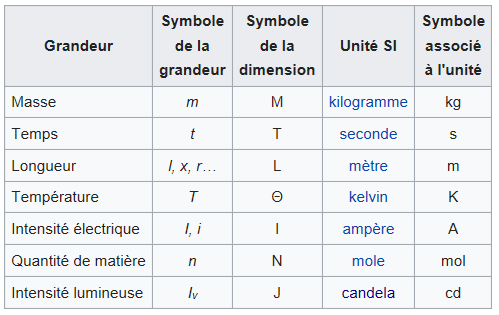
\includegraphics[height=6cm]{assets/figures/4_1_2_Systeme_international_d_unites_SI.PNG}
\caption{Système international d'unités SI: les 7 unités physiques de base.}
\label{fig:Systeme_international_d_unites_SI}
\end{figure}

\section{Choix d'un capteur}

Le choix du capteur approprié dépend du cahier des charges. Les conditions imposées sur la valeur à mesurer, imposent des caractéristiques métrologiques sur le capteur.
\begin {center}
\begin{tabular}{|p{6cm}|p{6cm}|}\hline
\textbf{MESURANDE} & \textbf{CAPTEUR} \\
Conditions imposées & Caractéristiques métrologiques \\\hline\hline
Plage de variation &	Etendue de mesure \\\hline
Variation minimale à mesurer & Résolution \\\hline
Spectre de fréquence ou vitesse de rotation  & Bande passante \\\hline
Précision de mesure	& Erreur de linéarité, Erreur d'hystérésis \\\hline
Plage de température de fonctionnement &	Dérive thermique du zéro, Tenue en température \\\hline
Localisation &	Encombrement \\\hline
Composition de l'atmosphère	 & Inertie chimique, Protection \\\hline
Parasites &	Blindage, Isolement ou non par rapport à la masse \\\hline
\end{tabular}
\end{center}
Source : www.geea.org

Ces conditions concernent autant le paramètre à mesurer (par exemple la pression) que l'environnement de mesure. Elles doivent être traduites en caractéristiques métrologiques du capteur. Ces caractéristiques sont à comparer à celles se trouvant dans les fiches techniques du capteur.

Le choix du bon capteur consiste à trouver des caractéristiques qui englobent les conditions imposées sur la mesurande.

\subsection{Principaux termes utilisés pour spécifier les capteurs}

Un grand nombre de paramètres spécifient un capteur. Ces paramètres sont identifiés par les termes du tableau ci-dessous.
\begin {center}
\begin{tabular}{|p{2.2cm}|p{2.8cm}|p{6.8cm}|p{2.4cm}|}
\hline
\textbf{Français} &	\textbf{Anglais} &	\textbf{Définition} &	\textbf{exemple} \\
\hline
\hline
Sensibilité &	Sensitivity &	output variation / input variation	 & mV/g, mA/oC \\
\hline
Stabilité &	Stability &	Coefficient de variation selon une grandeur d'influence &	stabilité en température \\
\hline
Précision &	Accuracy &	Somme de toutes les perturbations qui influencent la sortie du capteur	 &  \\
\hline
Etendue de mesure &	Span, range &	Valeur max mesurable - valeur min mesurable &	  \\
\hline
Résolution &	Resolution &	Plus petite variation du mesurande mesurable par le capteur &	  \\
\hline
Sélectivité &	Selectivity &	S'applique à des capteurs biochimiques, sensibles à une molécule plus particulièrement par rapport à une autre molécule &	  \\
\hline
Temps de réponse &	Response time &	Temps de propagation entre l'entrée et la sortie du capteur &	  \\
\hline
Conditions environnementales &	Environmental conditions &	Décrit les plages de variation admissible pour les paramètres extérieurs &	humidité, température, pression \\
\hline
Facteur de surcharge &	Overload characteristics &	Capacité à supporter un dépassement de la plage de mesure du mesurande & \\
\hline
Linearité &	Linearity & &	 	  \\
\hline
Hystérèse &	Hysteresis & &	 	  \\
\hline
Zone morte &	Dead band &	Plage de valeur du mesurande pour laquelle la sensibilité du capteur est nulle ou mauvaise &	 \\
\hline
Durée de vie &	Operating life &	Durée pendant laquelle les caractéristiques du capteur sont observées &	mtbf = mean time before failure \\
\hline
Taille & Size & &	 	  \\
\hline
Poids &	Weight & &	 	  \\
\hline
Prix &	Price & &	 	  \\
\hline
\end{tabular}
\end{center}

Il existe des capteurs actifs et passifs :
\begin{center}
\fbox{
\begin{minipage}{0.95\textwidth}
\textbf{\textit{Déf}. Capteur actif :}
n'a pas besoin d'énergie additionnelle: génère un signal électrique en réponse à un stimulus externe. Exemples: thermocouples, capteur pyroélectrique, capteur piézoélectrique. \\

\textbf{\textit{Déf}. Capteur passif :}
il s'agit généralement d'impédances. Les capteurs passifs nécessitent une énergie externe pour fonctionner, appelé signal d'excitation. Ce signal est modulé par le capteur pour produire le signal de sortie. Ces capteurs sont parfois appelés paramétriques, car leur signal de sortie change en fonction de ce signal d'excitation.
\end{minipage}
}
\end{center}

Les capteurs peuvent aussi être absolus ou relatifs, avec comme définitions :
\begin{center}
\fbox{
\begin{minipage}{0.95\textwidth}
\textbf{\textit{Déf}. Capteur absolu :}
détecte  un mesurande et produit une sortie en relation directe avec une échelle physique absolue indépendante des conditions de mesure. Exemple: résistance à coefficient de température positif, sa résistance dépend de la température absolue. \\

\textbf{\textit{Déf}. Capteur relatif :}
la sortie d'un capteur relatif dépend du contexte, d'une autre grandeur. Par exemple le signal de sortie d'un thermocouple ne peut être associé à une température absolue sans référencer l'une de ses extrémités à une température connue. Autre exemple, un capteur de pression peut être absolu lorsque son signal de sortie dépend de la différence entre la pression d'entrée et une pression de référence interne, ou relatif lorsqu'il est nécessaire d'appliquer une pression de référence de manière externe.
\end{minipage}
}
\end{center}

\section{Matériaux utilisés dans la réalisation de capteurs}

Différents matériaux sont utilisés pour la réalisation de capteurs.

\begin {center}
\begin{tabular}{|p{4.2cm}|p{9.5cm}|}
\hline
Organique &	Matière fabriquée par les êtres vivants \\
\hline
Inorganique &	Matière qui ne possède pas les caractéristiques nécessaires à la vie \\
\hline
Conducteur &	Corps capable de transmettre de l'électricité \\
\hline
Isolant &	Matériau qui isole de l'électricité \\
\hline
Semi-conducteur &	matériau qui a les caractéristiques électriques d'un isolant, mais pour lequel la probabilité qu'un électron puisse contribuer à un courant électrique, quoique faible, est suffisamment importante. En d'autres termes, la conductivité électrique d'un semi-conducteur est intermédiaire entre celle des métaux et celle des isolants \\
\hline
Liquide, gaz ou plasma &	Etats de la matière \\
\hline
Substance biologique &	Matériau extrait du monde vivant \\
\hline
\end{tabular}
\end{center}

\section{Principes de conversion}

Le mesurande doit être converti dans une grandeur exploitable. Cela nécessite un principe physique reliant cette grandeur au mesurande. Voici une liste non-exhaustive de principes physiques se retrouvant dans les capteurs :

\begin {center}
\begin{tabular}{|p{4.2cm}|p{9.5cm}|}
\hline
Physiques &	Piézoélectricité \\
\hline
 & 	Thermoélectrique \\
\hline
  &	Photoélectrique \\
\hline
 & 	Photomagnétique \\
\hline
 & 	Magnétoélectrique \\
\hline
 & 	Electromagnétique \\
\hline
 & 	Thermoélastique \\
\hline
 & 	Electroélastique \\
\hline
 & 	Thermomagnétique \\
\hline
 & 	Thermo-optique \\
\hline
 & 	Photoélastique \\
\hline
 & 	... \\
\hline
Chimiques &	Transformation chimique \\
\hline
 & 	Transformation physique \\
\hline
 & 	Processus électrochimique \\
\hline
 & 	Spectroscopie \\
\hline
 & 	... \\
\hline
Biologiques &	Transformation biochimique \\
\hline
 & 	Transformation physique \\
\hline
 & 	Effet sur un organisme de test \\
\hline
 & 	Spectroscopie \\
\hline
 & 	... \\
\hline
\end{tabular}
\end{center}

\section{Le mesurande}
Le mesurande est un terme défini comme étant la grandeur que l'on veut mesurer. La définition du mesurande est un préalable essentiel dans tout processus de mesure. Une liste non exhaustive de mesurandes :

%\begin{multicols}{2}
\begin {center}
\begin{tabular}{|p{3cm}|p{7cm}|}
\hline
Onde & acoustique	amplitude \\
\hline
 & 	phase \\
\hline
 & 	polarisation \\
\hline
 & 	spectre \\
\hline
 & 	vélocité \\
\hline
\end{tabular}
\begin{tabular}{|p{3cm}|p{7cm}|}
Biologique &	type de biomasse \\
\hline
 & 	concentration \\
\hline
 & 	états \\
\hline
\end{tabular}
\begin{tabular}{|p{3cm}|p{7cm}|}
Chimique &	type de composants \\
\hline
 & 	concentration \\
\hline
 & 	états \\
\hline
\end{tabular}
\begin{tabular}{|p{3cm}|p{7cm}|}
Electrique &	charge, courant \\
\hline
 & 	potentiel, tension \\
\hline
 & 	champ électrique \\
\hline
 & 	conductivité \\
\hline
 & 	permittivité \\
\hline
\end{tabular}
\begin{tabular}{|p{3cm}|p{7cm}|}
Magnétique &	amplitude \\
\hline
  &	phase \\
\hline
  &	polarisation \\
\hline
  &	spectre \\
\hline
  &	flux \\
\hline
  &	perméabilité \\
\hline
\end{tabular}
\begin{tabular}{|p{3cm}|p{7cm}|}
Onde optique &	amplitude \\
\hline
 & 	phase \\
\hline
 & 	polarisation \\
\hline
 & 	spectre \\
\hline
 & 	vélocité \\
\hline
 & 	indice de réfraction \\
\hline
 & 	émissivité \\
\hline
 & 	réflectivité \\
\hline
 & 	absorbtion \\
\hline
\end{tabular}
\begin{tabular}{|p{3cm}|p{7cm}|}
Mécanique &	position linéaire \\
\hline
 & 	position angulaire \\
\hline
 & 	force \\
\hline
 & 	tension, pression \\
\hline
 & 	contrainte \\
\hline
 & 	masse, densité \\
\hline
 & 	moment, couple \\
\hline
 & 	vitesse \\
\hline
 & 	forme, état de surface \\
\hline
 & 	orientation \\
\hline
 & 	cristalinité, structure \\
\hline
\end{tabular}
\begin{tabular}{|p{3cm}|p{7cm}|}
Radiation &	type \\
\hline
 & 	énergie \\
\hline
 & 	intensité \\
\hline
\end{tabular}
\begin{tabular}{|p{3cm}|p{7cm}|}
Thermique &	température \\
\hline
 & 	flux thermique \\
\hline
 & 	chaleur spécifique \\
\hline
 & 	conductvité thermique \\
\hline
\end{tabular}
\end{center}
~\\
%\end{multicols}

Le \textbf{mesurage}, c'est l'ensemble des opérations pour déterminer la valeur du mesurande, dont le résultat est la \textbf{mesure}.

Parfois, la valeur que l'on peut mesurer n'est pas la valeur que l'on veut mesurer. La grandeur mesurée n'est alors pas équivalente au mesurande. Par exemple, si les conditions de mesure ne sont pas adéquates, il est alors nécessaire d'effectuer une correction de la valeur mesurée. Exemple : en voulant mesurer la longueur d'une pièce mécanique à $20 \degree C$, alors que sa température réelle est de $80 \degree C$, il est nécessaire d'effectuer une correction due à la dilatation (entre $20 \degree C$ et $80 \degree C$).

\section{Capteur réel}
L'écart entre la valeur vraie et la valeur mesurée s'appelle l'erreur de mesure. Un capteur réel souffre de plusieurs erreurs caractéristiques (source : www.geea.org) :

\begin{figure}[h!]
\centering
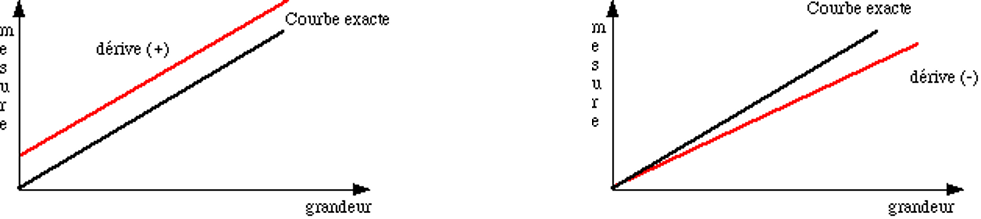
\includegraphics[width=\textwidth]{assets/figures/4_1_8_Erreurs_de_decalage_et_de_gain.PNG}
\caption{Erreurs de décalage et de gain}
\label{fig:Erreurs_de_decalage_et_de_gain}
\end{figure}

\begin{figure}[h!]
\centering
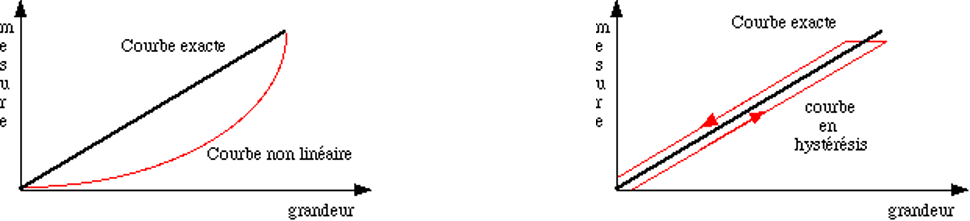
\includegraphics[width=\textwidth]{assets/figures/4_1_8_Erreurs_de_linearite_et_d_hysterese.PNG}
\caption{Erreurs de linéarité et d'hystérèse}
\label{fig:Erreurs_de_linearite_et_d_hysterese}
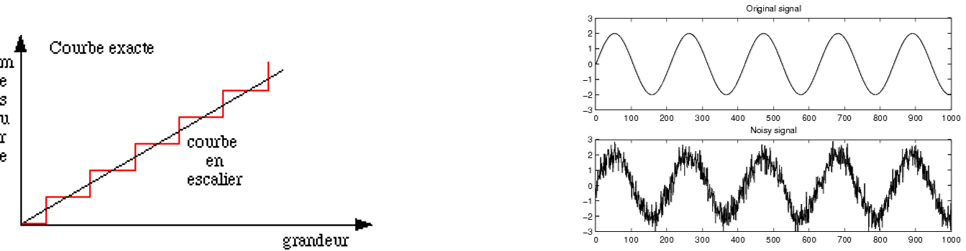
\includegraphics[width=\textwidth]{assets/figures/4_1_8_Erreurs_de_mobilite_et_bruit.PNG}
\caption{Erreurs de mobilité et bruit}
\label{fig:Erreurs_de_mobilite_et_bruit}
\end{figure}
Il faut en particulier différencier les erreurs systématiques et les erreurs aléatoires. L'erreur systématique est un décalage entre la valeur vraie et la valeur mesurée. L'erreur aléatoire peut se situer de part et d'autre de la valeur vraie.
\begin{figure}[h!]
\centering
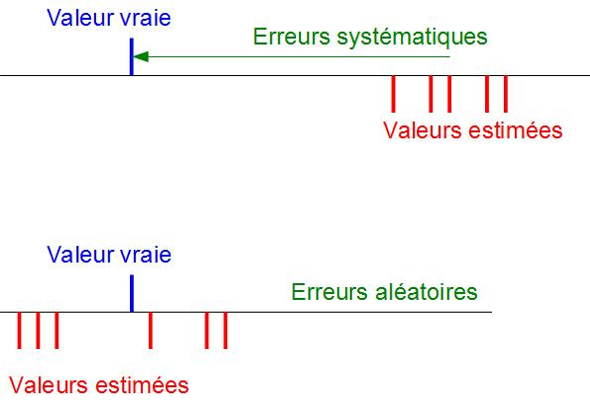
\includegraphics[height=6cm]{assets/figures/4_1_8_Erreurs_systematiques_et_aleatoires.PNG}
\caption{Erreurs systématiques et aléatoires}
\label{fig:Erreurs_systematiques_et_aleatoires}
\end{figure}
Les notions de justesse et de fidélité (ou répétabilité) sont associées à ces erreurs systématiques et aléatoires.

\section{Exemples de capteurs}

\subsection{Grandeurs électriques}

\subsubsection{Capteur de courant inductif}

Différent principaux permettent la mesure du courant électrique. Le transformateur de courant est une technique inductive basé sur un transformateur ayant au primaire une ou plusieurs spires avec le fil où la mesure de courant est effectuée. Au secondaire se trouve un ampèremètre. Le ratio entre le courant du secondaire et du primaire est proportionnel au rapport du nombre de spires entre le primaire et le secondaire.
\begin{figure}[h!]
\centering
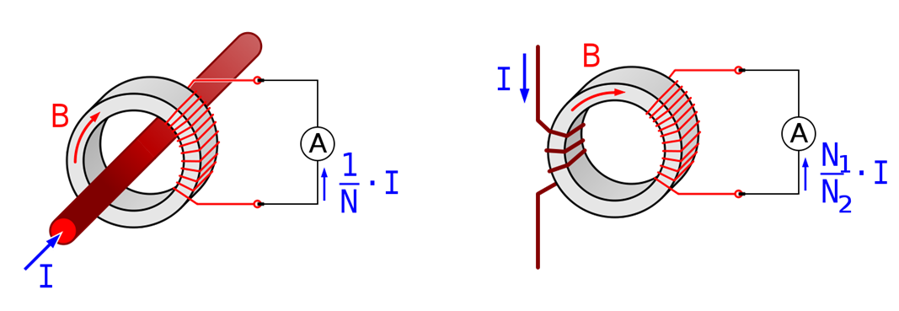
\includegraphics[height=5cm]{assets/figures/4_2_1_1_Capteur_de_courant_inductif.PNG}
\caption{Capteur de courant inductif (Source : Wikipedia).}
\label{fig:Capteur_de_courant_inductif}
\end{figure}

\subsubsection{Bobine de Rogowski}

La bobine de Rogowski est un cas particulier de mesure inductive sans entrefer. Il s'agit d'un solénoôde particulier placé autour du conducteur. La tension induite est peu/pas dépendante de la position du conducteur dans la boucle.

\begin{figure}[h!]
\centering
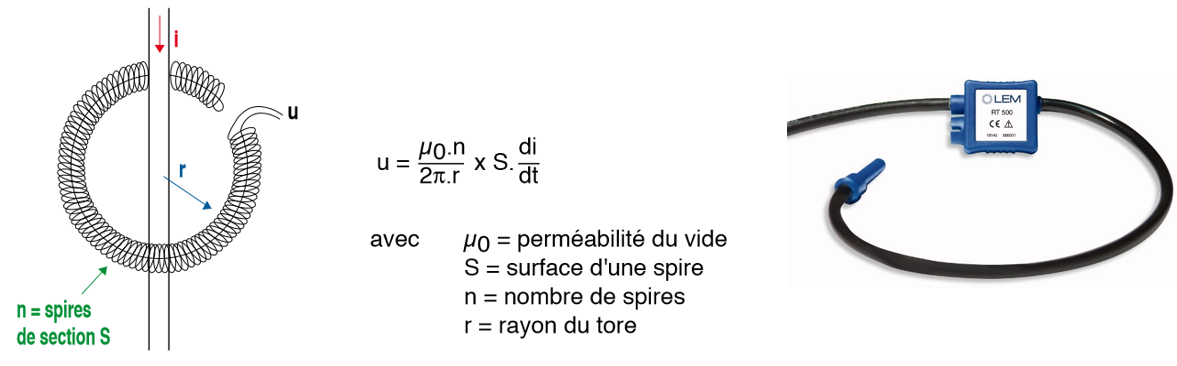
\includegraphics[width=15cm]{assets/figures/4_2_1_2_Bobine_de_Rogowski.PNG}
\caption{Bobine de Rogowski (Sources : Chauvin-Arnoux et LEM).}
\label{fig:Bobine_de_Rogowski}
\end{figure}


\subsubsection{Capteur de courant par effet Hall}
D'autres principes permettent de mesurer le courant, comme par exemple un capteur à effet Hall mesurant le champ magnétique autour du conducteur. Cette solution a comme gros avantage, par rapport aux techniques inductives, de permettre la mesure des courants continus.


\begin{figure}[h!]
\centering
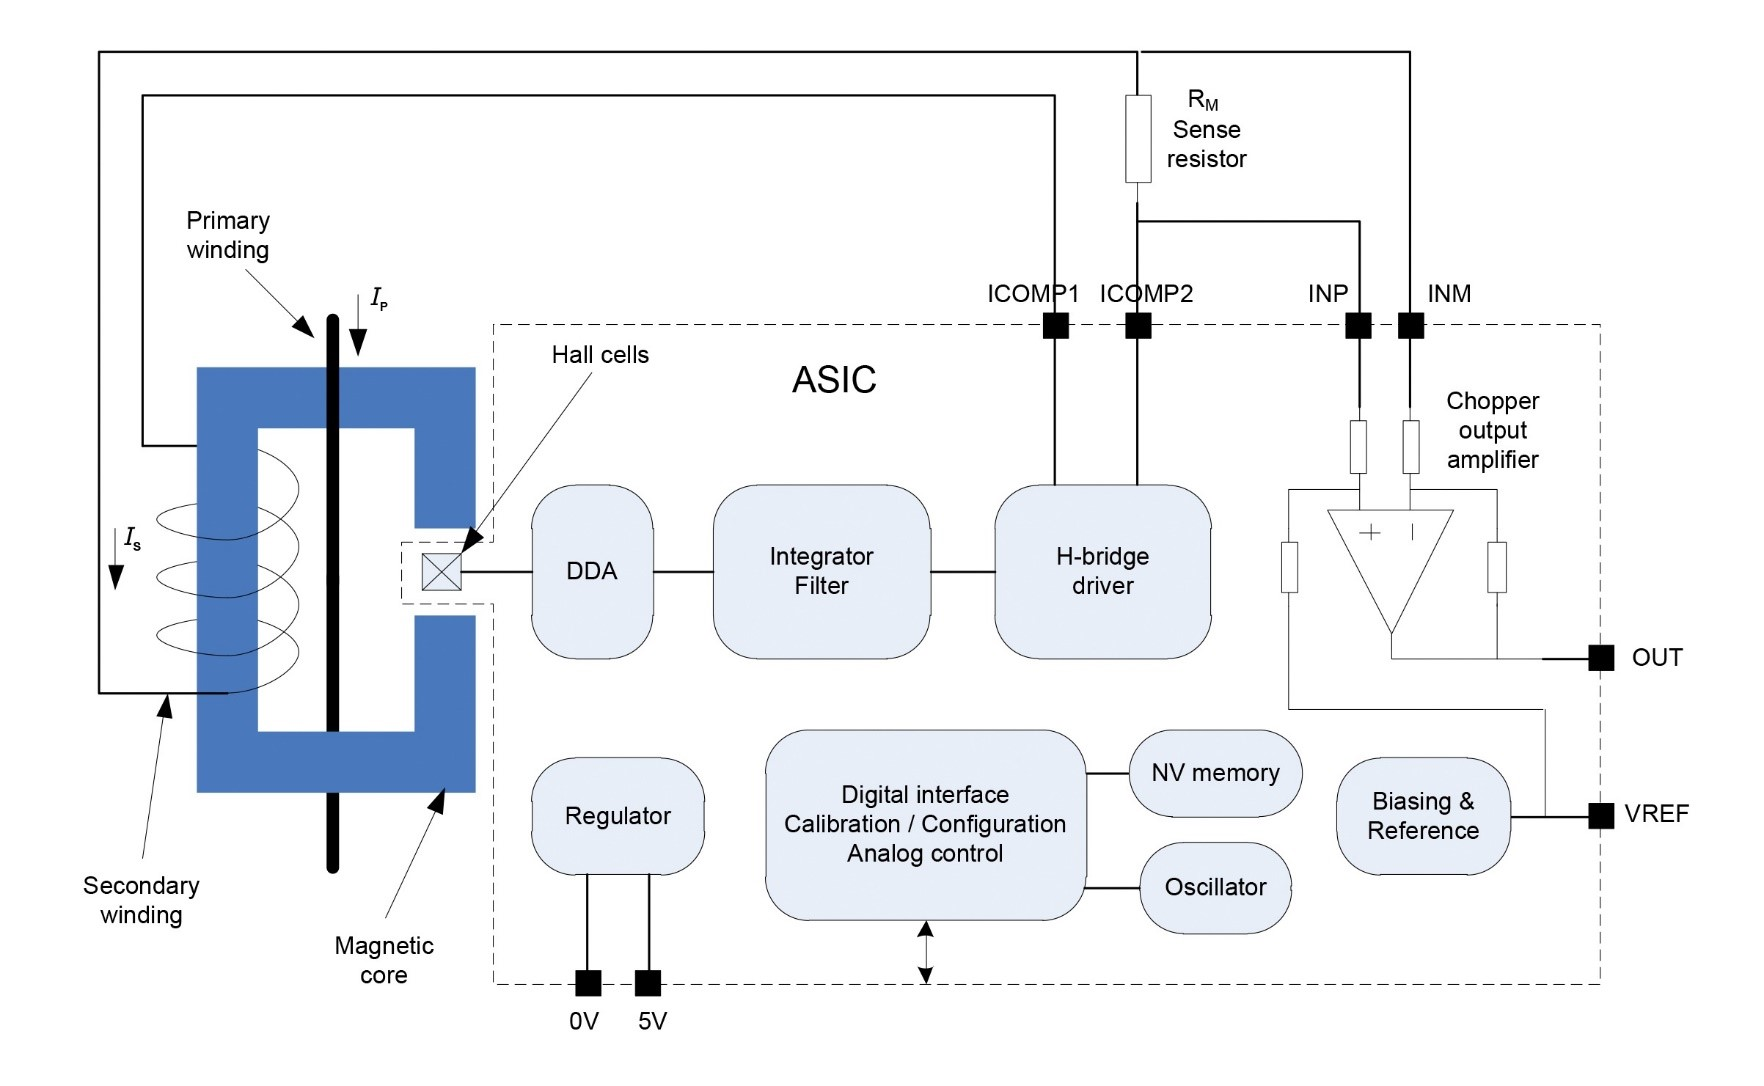
\includegraphics[width=15cm]{assets/figures/4_2_1_2_Capteur_de_courant_par_effet_Hall.jpg}
\caption{Capteur de courant par effet Hall (Source: LEM).}
\label{fig:Capteur_de_courant_par_effet_Hall}
\end{figure}

Ci-joint se trouve le schéma d'un capteur intelligent permettant la mesure en boucle fermée. Une contre-réaction permet de générer un champ magnétique s'opposant au champ magnétique lui-même généré par le courant à mesurer. Une structure à contre-réaction offre le grand avantage d'être sensible aux caractéristiques de la bobine plutôt qu'à la sensibilité du capteur à effet Hall.

\subsection{Température (TMP75 de Texas Instruments)}
Le TMP75 de Texas Instrument est un capteur intelligent disposant d'une interface I2C.

\begin{figure}[h!]
\centering
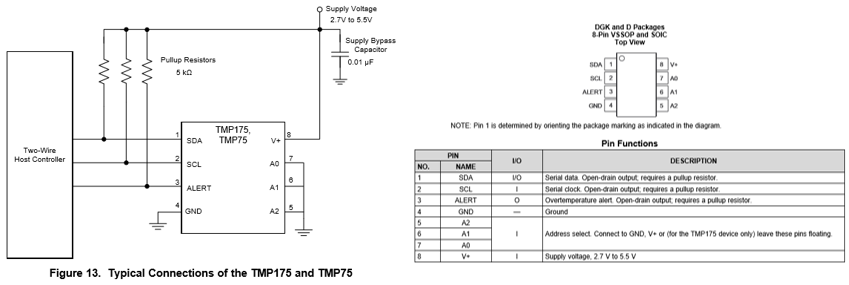
\includegraphics[width=15cm]{assets/figures/4_2_2_Temperature_TMP75.PNG}
\caption{Mesure de température avec le circuit TMP75}
\label{fig:Temperature_TMP75}
\end{figure}

Il se connecte aisément à un hôte, comme un microcontrôleur avec les deux signaux SDA et SCL. Une ligne supplémentaire ALERT permet en particulier de déclencher des interruptions.

Ce capteur intelligent dispose d'une cellule de mesure (Diode Temp. Sensor dans le schéma bloc ci-dessous), d'un convertisseur analogique-numérique (convertisseur $ \Delta \Sigma$) et numérique-analogique.


\begin{figure}[h!]
\centering
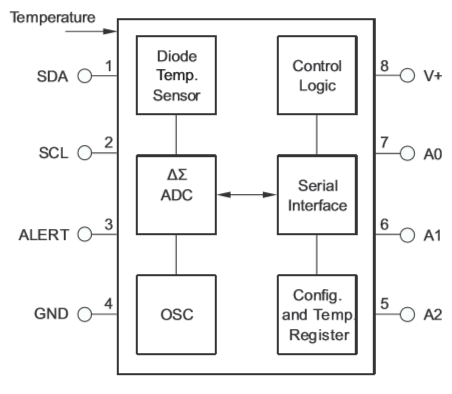
\includegraphics[height=6cm]{assets/figures/4_2_2_Temperature_TMP75_schema_bloc.PNG}
\caption{Schéma bloc circuit TMP75}
\label{fig:Temperature_TMP75_schema_bloc}
\end{figure}

Pour un capteur de température, la fiche technique donne un grand nombre de paramètres, comme en particulier les caractéristiques électriques ci-dessous. Chaque caractéristique peut avoir une grande importance pour une application.

\begin{figure}[h!]
\centering
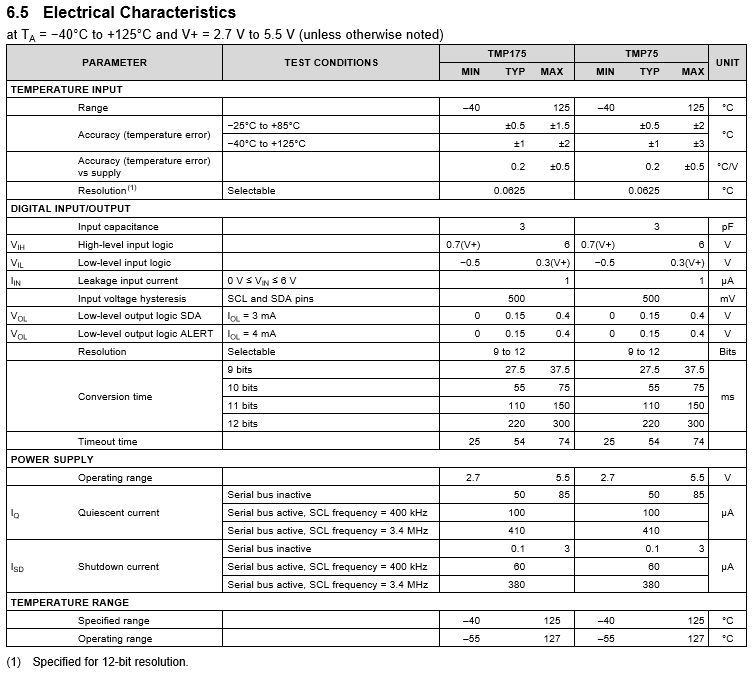
\includegraphics[width=15cm]{assets/figures/4_2_2_Temperature_TMP75_caracteristiques.PNG}
\caption{Caractéristiques du circuit TMP75}
\label{fig:Temperature_TMP75_caracteristiques}
\end{figure}



\subsection{Humidité (SHT3x-ARP de Sensirion)}
\begin{figure}[h!]
\centering
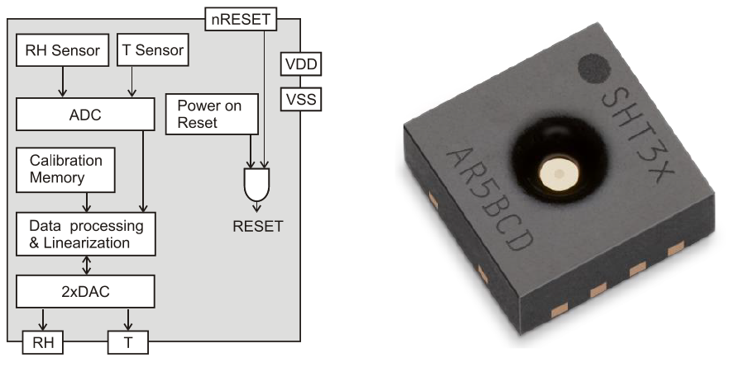
\includegraphics[width=8cm]{assets/figures/4_2_3_Humidite_SHT_3x_ARP.PNG}
\caption{Capteur d'humidité de Sensirion, SHT3x-ARP}
\label{fig:Humidite_SHT3x_ARP}
\end{figure}


La mesure de l'humidité avec ce capteur (Sensirion SHT3x-ARP) est une tension analogique ratiométrique 10\% to 90\%. Cela veut dire que la mesure est proportionnelle à la tension d'alimentation. A noter un deuxième signal de température.


\begin{figure}[h!]
\centering
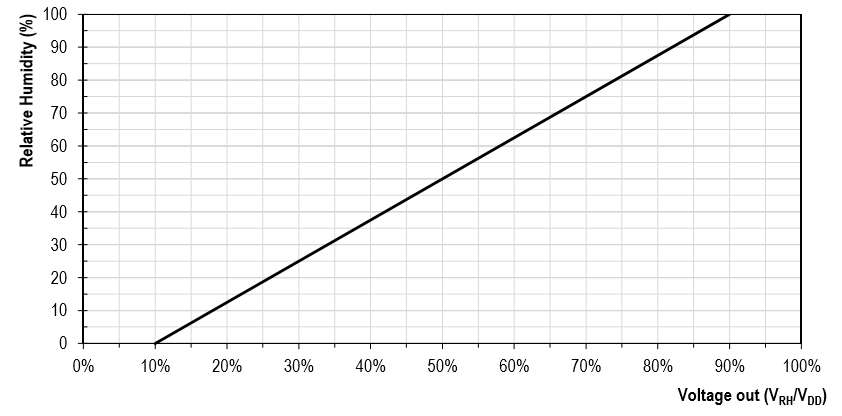
\includegraphics[width=15cm]{assets/figures/4_2_3_Humidite_SHT_3x_ARP_reponse.PNG}
\caption{Réponse du capteur d'humidité de Sensirion, SHT3x-ARP}
\label{fig:Humidite_SHT3x_ARP_reponse}
\end{figure}

L'incertitude de mesure se retrouve dans la fiche technique, avec une erreur typique et une erreur maximale.



\begin{figure}[h!]
\centering
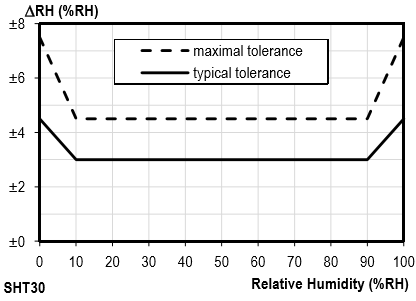
\includegraphics[width=10cm]{assets/figures/4_2_3_Humidite_SHT_3x_ARP_incertitude.PNG}
\caption{Incertitude de mesure du capteur d'humidité de Sensirion, SHT3x-ARP}
\label{fig:Humidite_SHT3x_ARP_incertitude}
\end{figure}

\subsection{Pression (Keller series 26 W)}
Le principe de fonctionnement de ce capteur de pression est une membrane se déformant sous l'effet de la différence de pression appliquée sur ces deux faces. Des piézorésistances (changement de résistance électrique d'un matériau dû à une contrainte mécanique) mesurent les contraintes mécaniques dans la membrane.


\begin{figure}[h!]
\centering
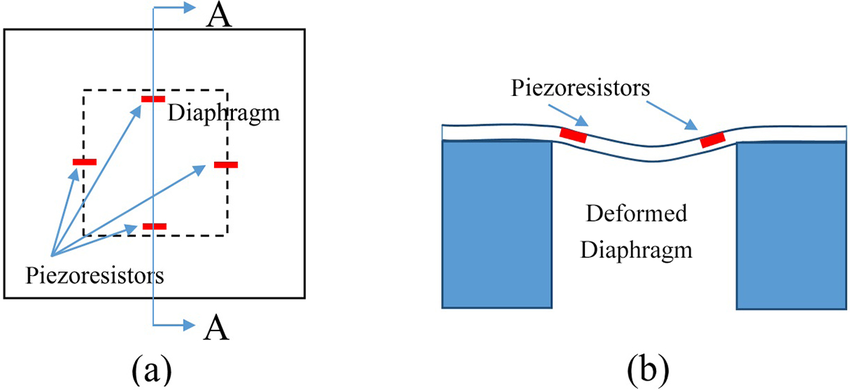
\includegraphics[width=10cm]{assets/figures/4_2_4_Pression_Keller_series26W.PNG}
\caption{Capteur de pression de Keller, series 26 W (Source : Kubba 2016)}
\label{fig:Pression_Keller_series26W}
\end{figure}

Ce capteur est utilisé pour mesurer des niveaux d'eau, indirectement en mesurant la pression due à la profondeur d'immersion. C'est la différence de pression avec la pression hors de l'eau qui est mesurée. Pour amener la pression atmosphérique au niveau de la membrane, un tuyau remonte en surface en passant dans le c‚ble (tube de ventilation).

\begin{figure}[h!]
\centering
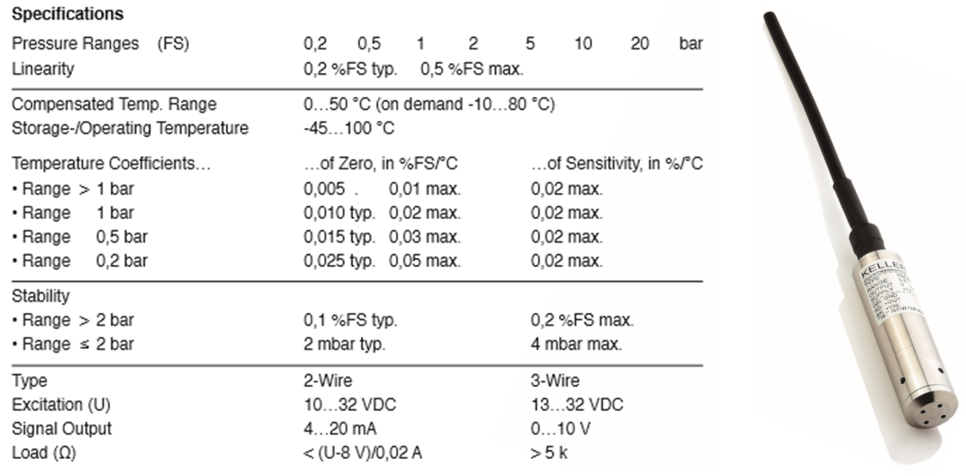
\includegraphics[width=15cm]{assets/figures/4_2_4_Pression_Keller_series26W_caracteristiques.PNG}
\caption{Caractéristiques du capteur de pression de Keller, series 26 W}
\label{fig:Pression_Keller_series26W_caracteristiques}
\end{figure}

\subsection{Jauges de déformation}
Dans une jauge, une déformation provoque une variation de la résistance. Cette variation de résistance répond à l'équation : \\
$\Delta R = k \ Delta L $
Avec :
$\Delta R$ : variation de résistance [$\Omega$]
$\Delta L$ : déformation [m]
k : coefficient ou facteur de jauge [$\Omega/m$]

\begin{figure}[h!]
\centering
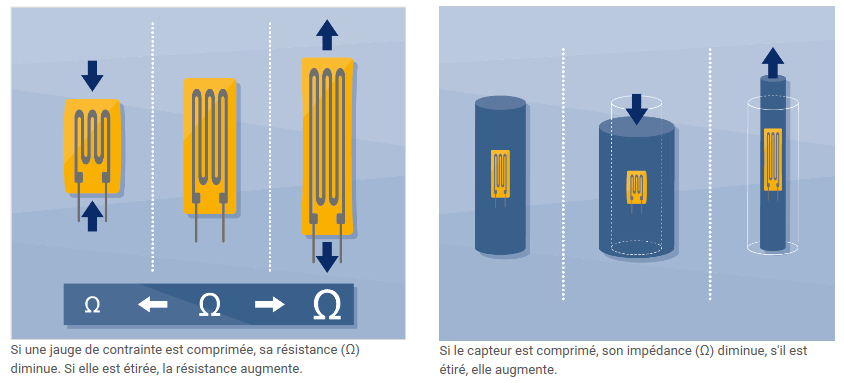
\includegraphics[width=15cm]{assets/figures/4_2_5_Jauges_de_deformation.png}
\caption{Jauges de déformation (source HBM)}
\label{fig:Jauges_de_deformation}
\end{figure}

Les jauges sont montées sur un corps d'épreuve. Les contraintes mécaniques entraînent une déformation. C'est cette déformation qui est mesurée par la jauge. Elle permet de retrouver la contrainte connaissant la rigidité du corps d'épreuve.


\subsection{Force (HBM RSCC)}

Les forces sont mesurées par la déformation d'un corps d'épreuve.
Pour ce capteur de force, des jauges de contraintes sont montées selon un pont de Wheastone sur les zones avec des contraintes mécaniques importantes et avec des paires où les contraintes mécaniques sont opposées (jauges 1-4 et 2-3).

\begin{figure}[h!]
\centering
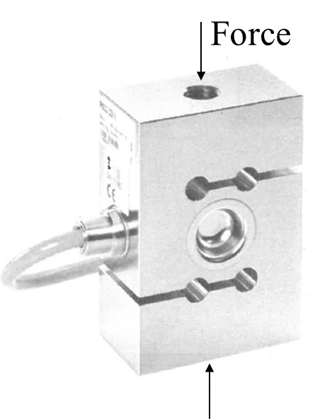
\includegraphics[width=7cm]{assets/figures/4_2_6_Force_HBM_RSCC.PNG}
\caption{Capteur de Force HBM RSCC (source HBM)}
\label{fig:Force_HBM_RSCC}
\end{figure}

\begin{figure}[h!]
\centering
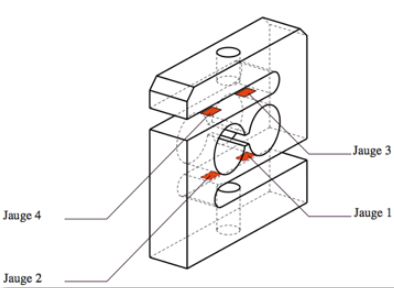
\includegraphics[width=7cm]{assets/figures/4_2_6_Force_HBM_RSCC_detail.PNG}
\caption{Capteur de Force HBM RSCC: détails}
\label{fig:Force_HBM_RSCC_detail}
\end{figure}

Le pont de Wheastone est composé de 4 résistances. Ces résistances sont remplacées par des jauges, avec une, deux ou quatre jauges, respectivement pour un quart de pont, demi-pont ou pont complet.
\begin{figure}[h!]
\centering
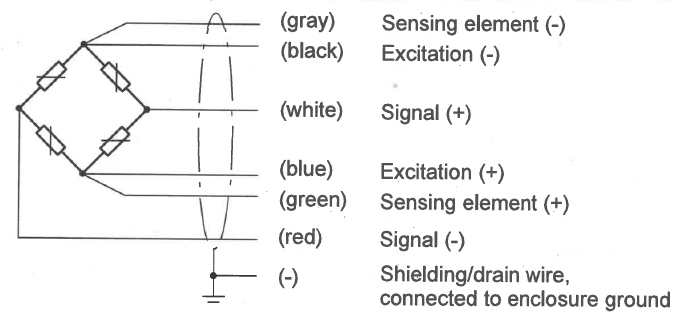
\includegraphics[width=7cm]{assets/figures/4_2_6_Force_HBM_RSCC_connexions.PNG}
\caption{Capteur de Force HBM RSCC: connexions}
\label{fig:Force_HBM_RSCC_connexions}
\end{figure}

\subsection{Couple (Omega TQ513)}
L'Omega TQ513 est un capteur de couple, basé sur des jauges de contraintes, placées sur une zone déformable (corps d'épreuve). Les jauges étant sur la partie tournante, un dispositif permet d'assurer le contact électrique glissant (slip rings).

\begin{figure}[h!]
\centering
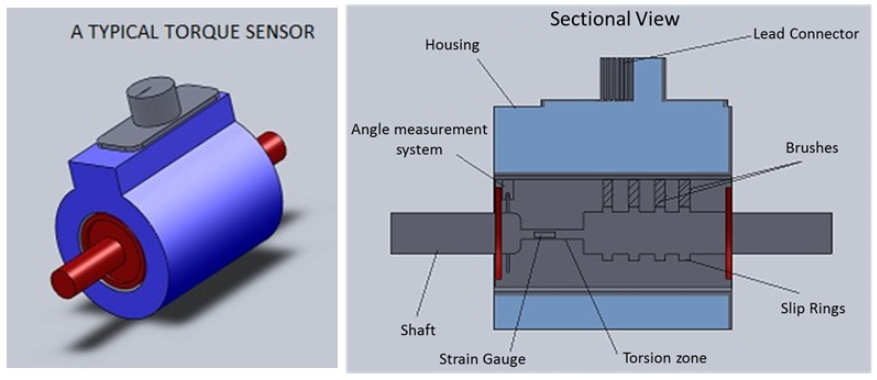
\includegraphics[width=7cm]{assets/figures/4_2_7_Couple_Omega_TQ513.PNG}
\caption{Capteur de couple: Omega TQ513}
\label{fig:Couple_Omega_TQ513}
\end{figure}

La déformation est liée aux propriétés mécaniques de la zone de torsion. Les jauges sont placées dans les axes de déformation maximale. Pour un pont complet, il y a une paire de jauge en compression et une paire en extension.


\begin{figure}[h!]
\centering
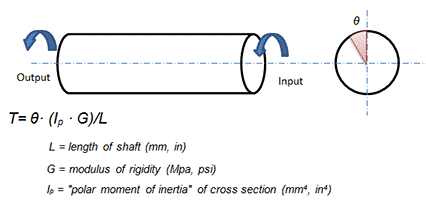
\includegraphics[width=7cm]{assets/figures/4_2_7_Couple_Omega_TQ513_principe.PNG}
\caption{Principe du capteur de couple (Source : https://cecas.clemson.edu)}
\label{fig:Couple_Omega_TQ513_principe}
\end{figure}

\subsection{Position linéaire (LT1300)}
Les capteurs LT1300 est un capteur de position linéaire, avec une gamme de 25 à 200mm.


\begin{figure}[h!]
\centering
\includegraphics[width=7cm]{assets/figures/4_2_8_Position_lineaire_LT1300.PNG}
\caption{Capteur de position linéaire LT1300}
\label{fig:Position_lineaire_LT1300}
\end{figure}

Il fonctionne sur le principe du LVDT. C'est un principe inductif, utilisant un noyau ferromagnétique se déplaçant dans un transformateur pour modifier les couplages. Il utilise deux secondaires afin d'obtenir une réponse symétrique.

\begin{figure}[h!]
\centering
\includegraphics[width=7cm]{assets/figures/4_2_8_Position_lineaire_LT1300_detail.PNG}
\caption{Capteur de position linéaire LT1300: principe}
\label{fig:Position_lineaire_LT1300_detail}
\end{figure}

Un conditionneur de signal est nécessaire pour l'excitation du LVDT et pour effectuer la mesure. A noter que la réponse des LVDT n'est pas très linéaire, ce qui nécessite souvent une linéarisation.

\begin{figure}[h!]
\centering
\includegraphics[width=7cm]{assets/figures/4_2_8_Position_lineaire_LT1300_conditionneur.PNG}
\caption{Capteur de position linéaire LT1300: conditionneur}
\label{fig:Position_lineaire_LT1300_conditionneur}
\end{figure}

\subsection{Position angulaire (Baumer GM400)}
Le Baumer GM400 est un codeur absolu. Il utilise un principe optique. Un disque codé avec des trous, tournant avec l'axe, permet de mesurer la position angulaire grâce à une source lumineuse est des photodétecteurs.

\begin{figure}[h!]
\centering
\includegraphics[width=7cm]{assets/figures/4_2_9_Position_angulaire_Baumer_GM400.PNG}
\caption{Position angulaire Baumer GM400 (Sources : Baumer et Guy Gauthier)}
\label{fig:Position_angulaire_Baumer_GM400}
\end{figure}

Pour certains codeurs optiques, le code binaire Gray est utilisé. Ce code offre l'avantage de ne modifier qu'un seul bit à la fois quand un nombre est augmenté d'une unité, contrairement au codage binaire naturel. Cela permet d'éviter des états transitoires lors des transitions.


\begin{figure}[h!]
\centering
\includegraphics[width=7cm]{assets/figures/4_2_9_Position_angulaire_Baumer_GM400_codage.PNG}
\caption{Position angulaire Baumer GM400: codage}
\label{fig:Position_angulaire_Baumer_GM400_codage}
\end{figure}


Le transcodage binaire Gray/naturel est évidemment possible avec des algorithmes simples.

A noter que pour un capteur incrémental, deux signaux sont nécessaire pour connaître le sens de rotation. L'idée est d'utiliser deux signaux carrés déphasés de $90 \degree$.


\begin{figure}[h!]
\centering
\includegraphics[width=7cm]{assets/figures/4_2_9_Position_angulaire_Baumer_GM400_fonctionnement.PNG}
\caption{Position angulaire Baumer GM400: fonctionnement}
\label{fig:Position_angulaire_Baumer_GM400_fonctionnement}
\end{figure}

\subsection{Vitesse (Philips KMI15/1)}
Le capteur de vitesse Philips KMI15/1 utilise un principe magnétique, avec une roue dentée ferromagnétique déformant le champ magnétique d'un aimant permanent.



\begin{figure}[h!]
\centering
\includegraphics[width=7cm]{assets/figures/4_2_10_Vitesse_Philips_KMI15_1.PNG}
\caption{Capteur de vitesse: Philips KMI15/1}
\label{fig:Vitesse_Philips_KMI15_1}
\end{figure}

Le capteur KMI15/1 comprend l'aimant permanent et un capteur magnétorésitif (dont la résistance varie avec la magnétisation). La sortie du capteur est numérique de type tout ou rien (TOR).


\begin{figure}[h!]
\centering
\includegraphics[width=7cm]{assets/figures/4_2_10_Vitesse_Philips_KMI15_1_detail.PNG}
\caption{Détail du capteur de vitesse Philips KMI15/1}
\label{fig:Vitesse_Philips_KMI15_1_detail}
\end{figure}

A noter encore que la mesure de vitesse avec une roue dentée est aussi possible en utilisant des capteurs de technologie inductive ou optique.


\subsection{Capteur de vibration (Colibrys VS1000)}

Le capteur de vibration Colibrys VS1000 est base sur une masse suspendue. Un principe capacitif permet de mesurer la position de la masse ou de créer des forces (pour le self-test)
Ce capteur dispose d'une sortie analogique ratiométrique différentielle. Il dispose aussi d'une entrée pour lancer le self-test et d'un signal d'erreur en sortie. A noter encore la présence d'une mesure de température, souvent présente dans les capteurs intelligents.



\begin{figure}[h!]
\centering
\includegraphics[width=7cm]{assets/figures/4_2_11_Capteur_de_vibration_Colibrys_VS1000.PNG}
\caption{Capteur de vibration: Colibrys VS1000}
\label{fig:Capteur_de_vibration_Colibrys_VS1000}
\end{figure}

\subsection{Capteur de proximité (Baumer CFDK 30N3600)}

Le capteur Baumer CFDK 30N3600 est un capteur de proximité capacitif. Il permet de détecter sans contact des objets métalliques et non-métalliques à faible distance. Il permet aussi de détecter des niveaux de liquide à travers un réservoir. Un potentiomètre permet de régler la sensibilité du détecteur.

Ces capteurs de proximité disposent d'une sortie tout ou rien (TOR).

\subsection{Capteur chimique (Membrapor  CO/C-200)}

Les capteurs Membrapor  CO/C-200 sont des capteurs électrochimiques permettant la mesure de la concentration de monoxyde de carbone (CO). Pour ce type de capteurs, les dérives sont importantes, en particulier la dérive thermique, comme le montrent les graphiques ci-dessous.

\begin{figure}[h!]
\centering
\includegraphics[width=7cm]{assets/figures/4_2_13_Capteur_chimique_Membrapor_CO_C_200.PNG}
\caption{Capteur chimique: Membrapor  CO/C-200}
\label{fig:Capteur_chimique_Membrapor_CO_C_200}
\end{figure}

A noter encore des grandeurs d'influence (cross-sensitivity) provenant d'autres gaz.

\begin{figure}[h!]
\centering
\includegraphics[width=7cm]{assets/figures/4_2_13_Capteur_chimique_Membrapor_CO_C_200_performance.PNG}
\caption{Capteur chimique Membrapor  CO/C-200: performances}
\label{fig:Capteur_chimique_Membrapor_CO_C_200_performance}
\end{figure}

\subsection{Capteur optique (Hamamatsu S-4251)}

Le capteur optique Hamamatsu S-4251 est constitué d'un driver pour une led exerne, une photodiode (c'est la raison du boîtier transparent) et une électronique de mesure utilisant le principe de la détection synchrone.

\begin{figure}[h!]
\centering
\includegraphics[width=7cm]{assets/figures/4_2_14_Capteur_optique_Hamamatsu_S_4251.PNG}
\caption{Capteur optique:Hamamatsu S-4251}
\label{fig:Capteur_optique_Hamamatsu_S_4251}
\end{figure}

Il y a souvent dans les capteurs des composantes de bruit à basses fréquences (bruit 1/f ou de la dérive). Il y a aussi souvent la présence de perturbations à basse fréquence. Par exemple des variations lentes de la lumière ambiante ou un scintillement à 50Hz. Le principe de la détection synchrone consiste à moduler le signal à mesurer pour se retrouver avec une fréquence plus élevées que ces bruits à basse fréquence.

\begin{figure}[h!]
\centering
\includegraphics[width=7cm]{assets/figures/4_2_14_Capteur_optique_Hamamatsu_S_4251_conditionneur.PNG}
\caption{Capteur optique Hamamatsu S-4251: exemple de conditionneur (source: Analog Devices)}
\label{fig:Capteur_optique_Hamamatsu_S_4251_conditionneur}
\end{figure}

Dans ce capteur, le principe consiste à moduler la lumière vers 10kHz. Le signal reçu est alors démodulé en phase. Cela permet de s'affranchir de toutes les composantes de bruit à plus basse fréquence.

\subsection{Lectures conseillées}

\begin{itemize}\itemsep1pt
\renewcommand{\labelitemi}{$\bullet$}
\item " Les capteurs en instrumentation industrielle ", Georges Asch et Bernard Poussery, Dunod, 2017.
\item " Acquisition de données, du capteur à l'ordinateur ", Gorge Asch, Dunod, 2011.
\end{itemize}

%\end{document}
